\chapter{Measurement}\label{ch:measurement}
The purpose of this section is to characterize a power amplifier for its ACPR and AM/AM distortion and afterwards measure the impact of the crosstalk from the antennas. 

\section{Simulation of PCB antenna}
The antenna used for measurement is a PCB antenna that measures 100x300mm on standard 1.6mm FR-4. The antenna has a $S_{11}$ below -10dB from 2.5GHz to 6.0GHz and only gets as high as -7.5dBi all the way up to 10GHz. The antenna is linear polarized and has a transmit and receive gain at 11.4dB. On the front of the PCB a large copper area is presented. This copper area is feed from the backside of the PCB where a small track is feed with a sma connector. In the simulation this track is feed with a wave guide port.  
   
\begin{figure}[H]
  \centering
  \begin{minipage}[b]{0.5\textwidth}
	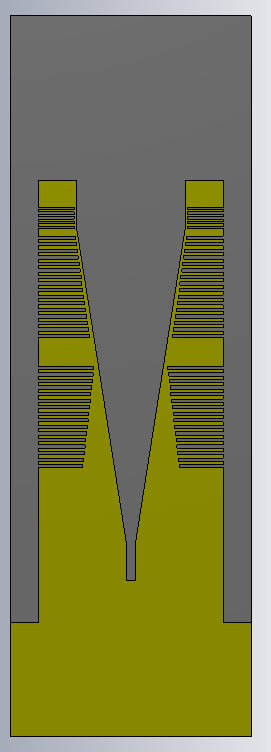
\includegraphics[scale = 0.5]{figures/measurement/antenna_front.png}
	\caption{Front of PCB antenna}
    \label{fig:ant_front}
  \end{minipage}
  \hfill
  \begin{minipage}[b]{0.4\textwidth}
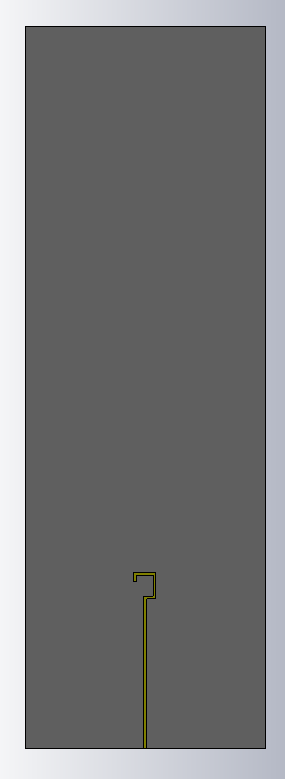
\includegraphics[scale = 0.5]{figures/measurement/antenna_back.png}
\caption{Backside of PCB antenna}
    \label{fig:ant_back}
  \end{minipage}
\end{figure}


\begin{figure}[H]
\centering 
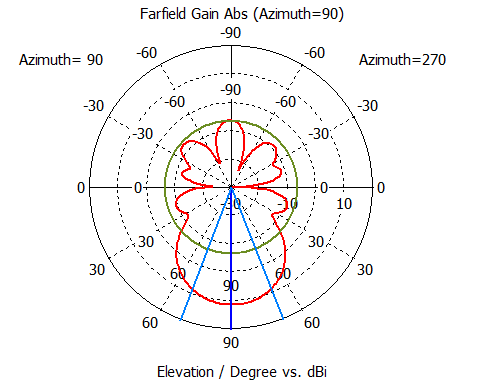
\includegraphics[scale = 0.7]{figures/measurement/antenna_ff.png}
\caption{Farfield of the antenna}
\label{fig:ant_ff}
\end{figure} 


\begin{figure}[H]
\centering 
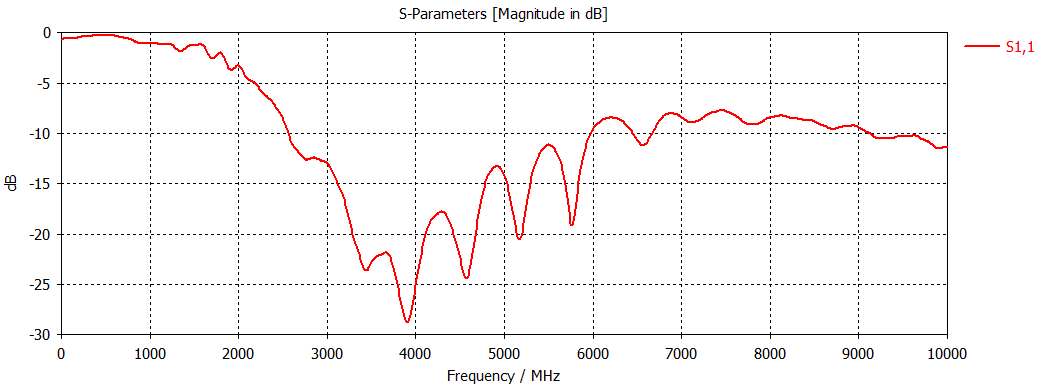
\includegraphics[scale = 0.6]{figures/measurement/antenna_spar.png}
\caption{$S_{11}$ of the antenna}
\label{fig:ant_spar}
\end{figure} 

\begin{figure}[H]
\centering 
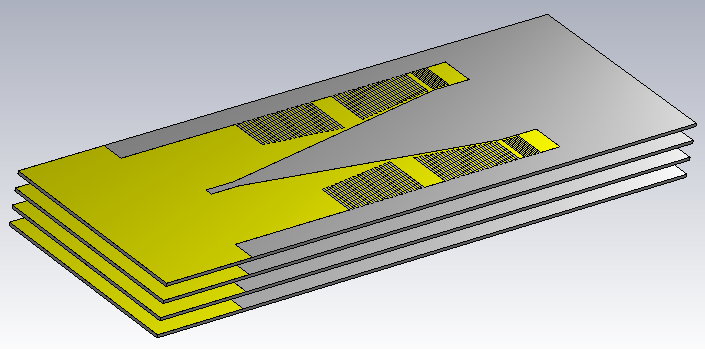
\includegraphics[scale = 0.7]{figures/measurement/antenna_array.png}
\caption{4 wideband PCB antennas separated $0.1\lambda = 8.6mm$ }
\label{fig:ant_array}
\end{figure}

\todo[inline]{insert s-par marix}
\section{Power Amplifier}
The  \textit{ZX60-6013E+} amplifier is a small buffer-amplifier with a BW from 20MHz - 6GHz. It has an output-power at maximum 11.16dBm at 3.5GHz (1 dB compression ). The gain is 13.85 dB and the noise figure is 3.42dB. In figure \ref{fig:amp_gain} and \ref{fig:amp_outpower} curves for the amplifier gain and output power versus frequency it depicted respectively. The amplifier is shown in figure \ref{fig:amplifier} 

\begin{figure}[H]
\centering 
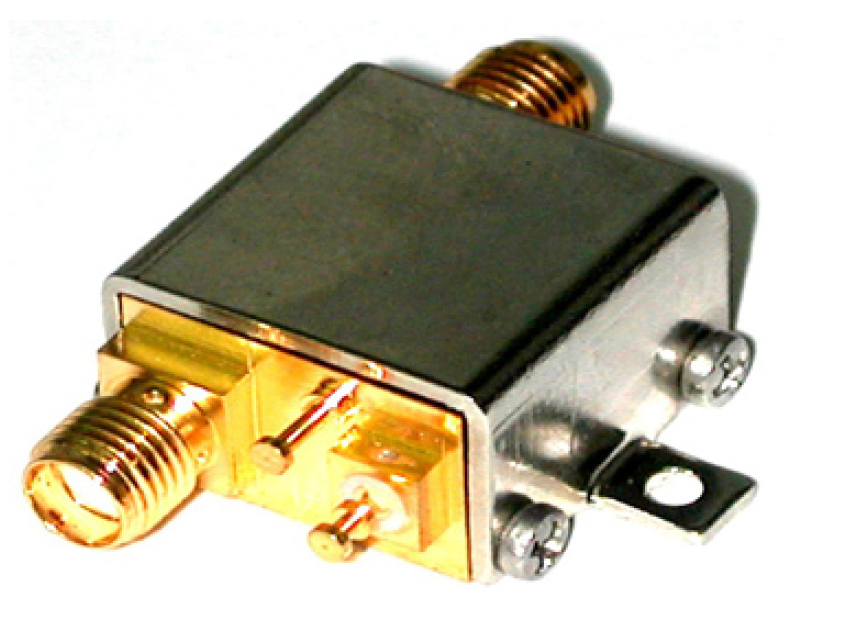
\includegraphics[scale = 0.3]{figures/measurement/amplifier.png}
\caption{The \textit{ZX60-6013E+} amplifier}
\label{fig:amplifier}
\end{figure} 

\begin{figure}[H]
  \centering
  \begin{minipage}[b]{0.5\textwidth}
	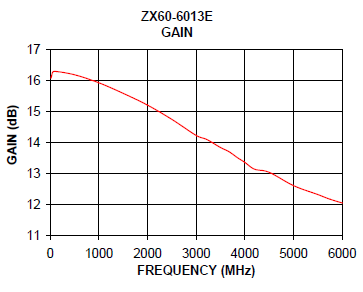
\includegraphics[scale = 0.7]{figures/measurement/amp_gain.png}
	\caption{Gain versus frequency}
    \label{fig:amp_gain}
  \end{minipage}
  \hfill
  \begin{minipage}[b]{0.4\textwidth}
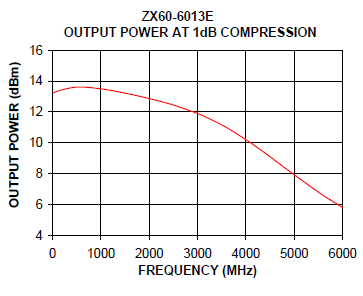
\includegraphics[scale = 0.7]{figures/measurement/amp_outpower.png}
\caption{Output power versus frequency}
    \label{fig:amp_outpower}
  \end{minipage}
\end{figure}


\section{Measurement setup} \label{ch_meas_setup}
To measure the impact of the antenna crosstalk, several measurements must be done at different setups. The first setup is shown in figure \ref{fig:Meas_setup1}. In this setup only the amplifier is measured. The signal generator is generating a 10MHz LTE signal at 3.5GHz where the output is connected to the input of the amplifier. The amplifier is supplied with a 12.0VDC signal from the power supply and the output of the amplifier is connected to a 6dB attenuator to protect the input stage of the spectrum analyser, which measures the output signal from the amplifier.   

\begin{figure}[H]
\centering 
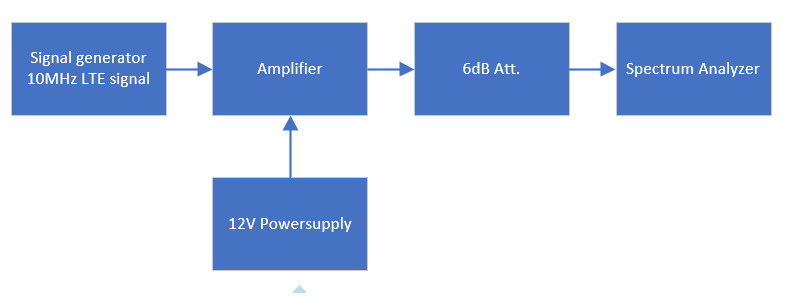
\includegraphics[scale = 0.6]{figures/measurement/meas_set_1.png}
\caption{Block diagram of measurement at amplifier }
\label{fig:Meas_setup1}
\end{figure} 

In figure \ref{fig:Meas_setup2} the second measurement setup is shown. In this setup the antennas are now introduced. The Tx antenna is connected to the output of the amplifier. The Rx antenna are spaced 1 meter apart from the Tx antenna (measured from feed to feed). The 6dB attenuator is removed and the antenna is connected to the spectrum analyzer. 


\begin{figure}[H]
\centering 
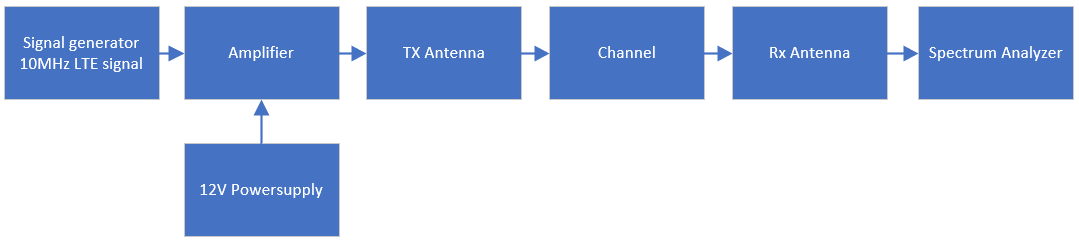
\includegraphics[scale = 0.6]{figures/measurement/meas_set_2.png}
\caption{Block diagram of measurement using one antenna}
\label{fig:Meas_setup2}
\end{figure} 

In setup three a power-divider is now introduced together with a second amplifier and second antenna. The received power will now increase 3dB but because the amplifiers has to be driven in the same power levels as before, one must add another 3dB to the input of the power divider. Be aware that in the measurements a 1:4 power divider was used and therefore the power was increased 6dB. The unused ports was terminated to a $50\Omega$ load. Also measurement using 4 antennas has been done in the same way. The only diffrence from the measurement was that the terminations was removed and an other 2 amplifiers and 2 antennas was added. See figure \ref{fig:Meas_setup4nt}.

\begin{figure}[H]
\centering 
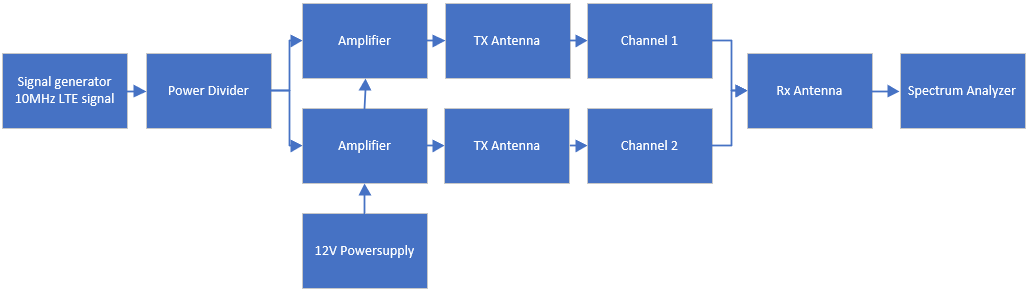
\includegraphics[scale = 0.6]{figures/measurement/meas_set_3.png}
\caption{Block diagram of measurement using two antennas}
\label{fig:Meas_setup3}
\end{figure} 


In figure \ref{fig:Meas_setup} a picture of a real measurement setup is shown. The antennas are spaced 1 meter apart from the input terminals and are pointing directly towards each other. The PA is mounted on a aluminium sheet with a tool grip to keep it at a constant temperature. The PA is supplied with 12.0VDC from the power supply and draws 40mA of current. The signal generator is connected to the input of the amplifier and the output of the amplifier is connected to the Tx antenna. The spectrum analyser is connected to Rx antenna. In figure \ref{fig:Meas_setup4ant} a measurement with 4 antennas is depicted. The antennas is mounted in a piece of flamingo with slots at at distance of $0.1\lambda$. This way the antenna can be moved to make the desired measurement.   


\begin{figure}[H]
\centering 
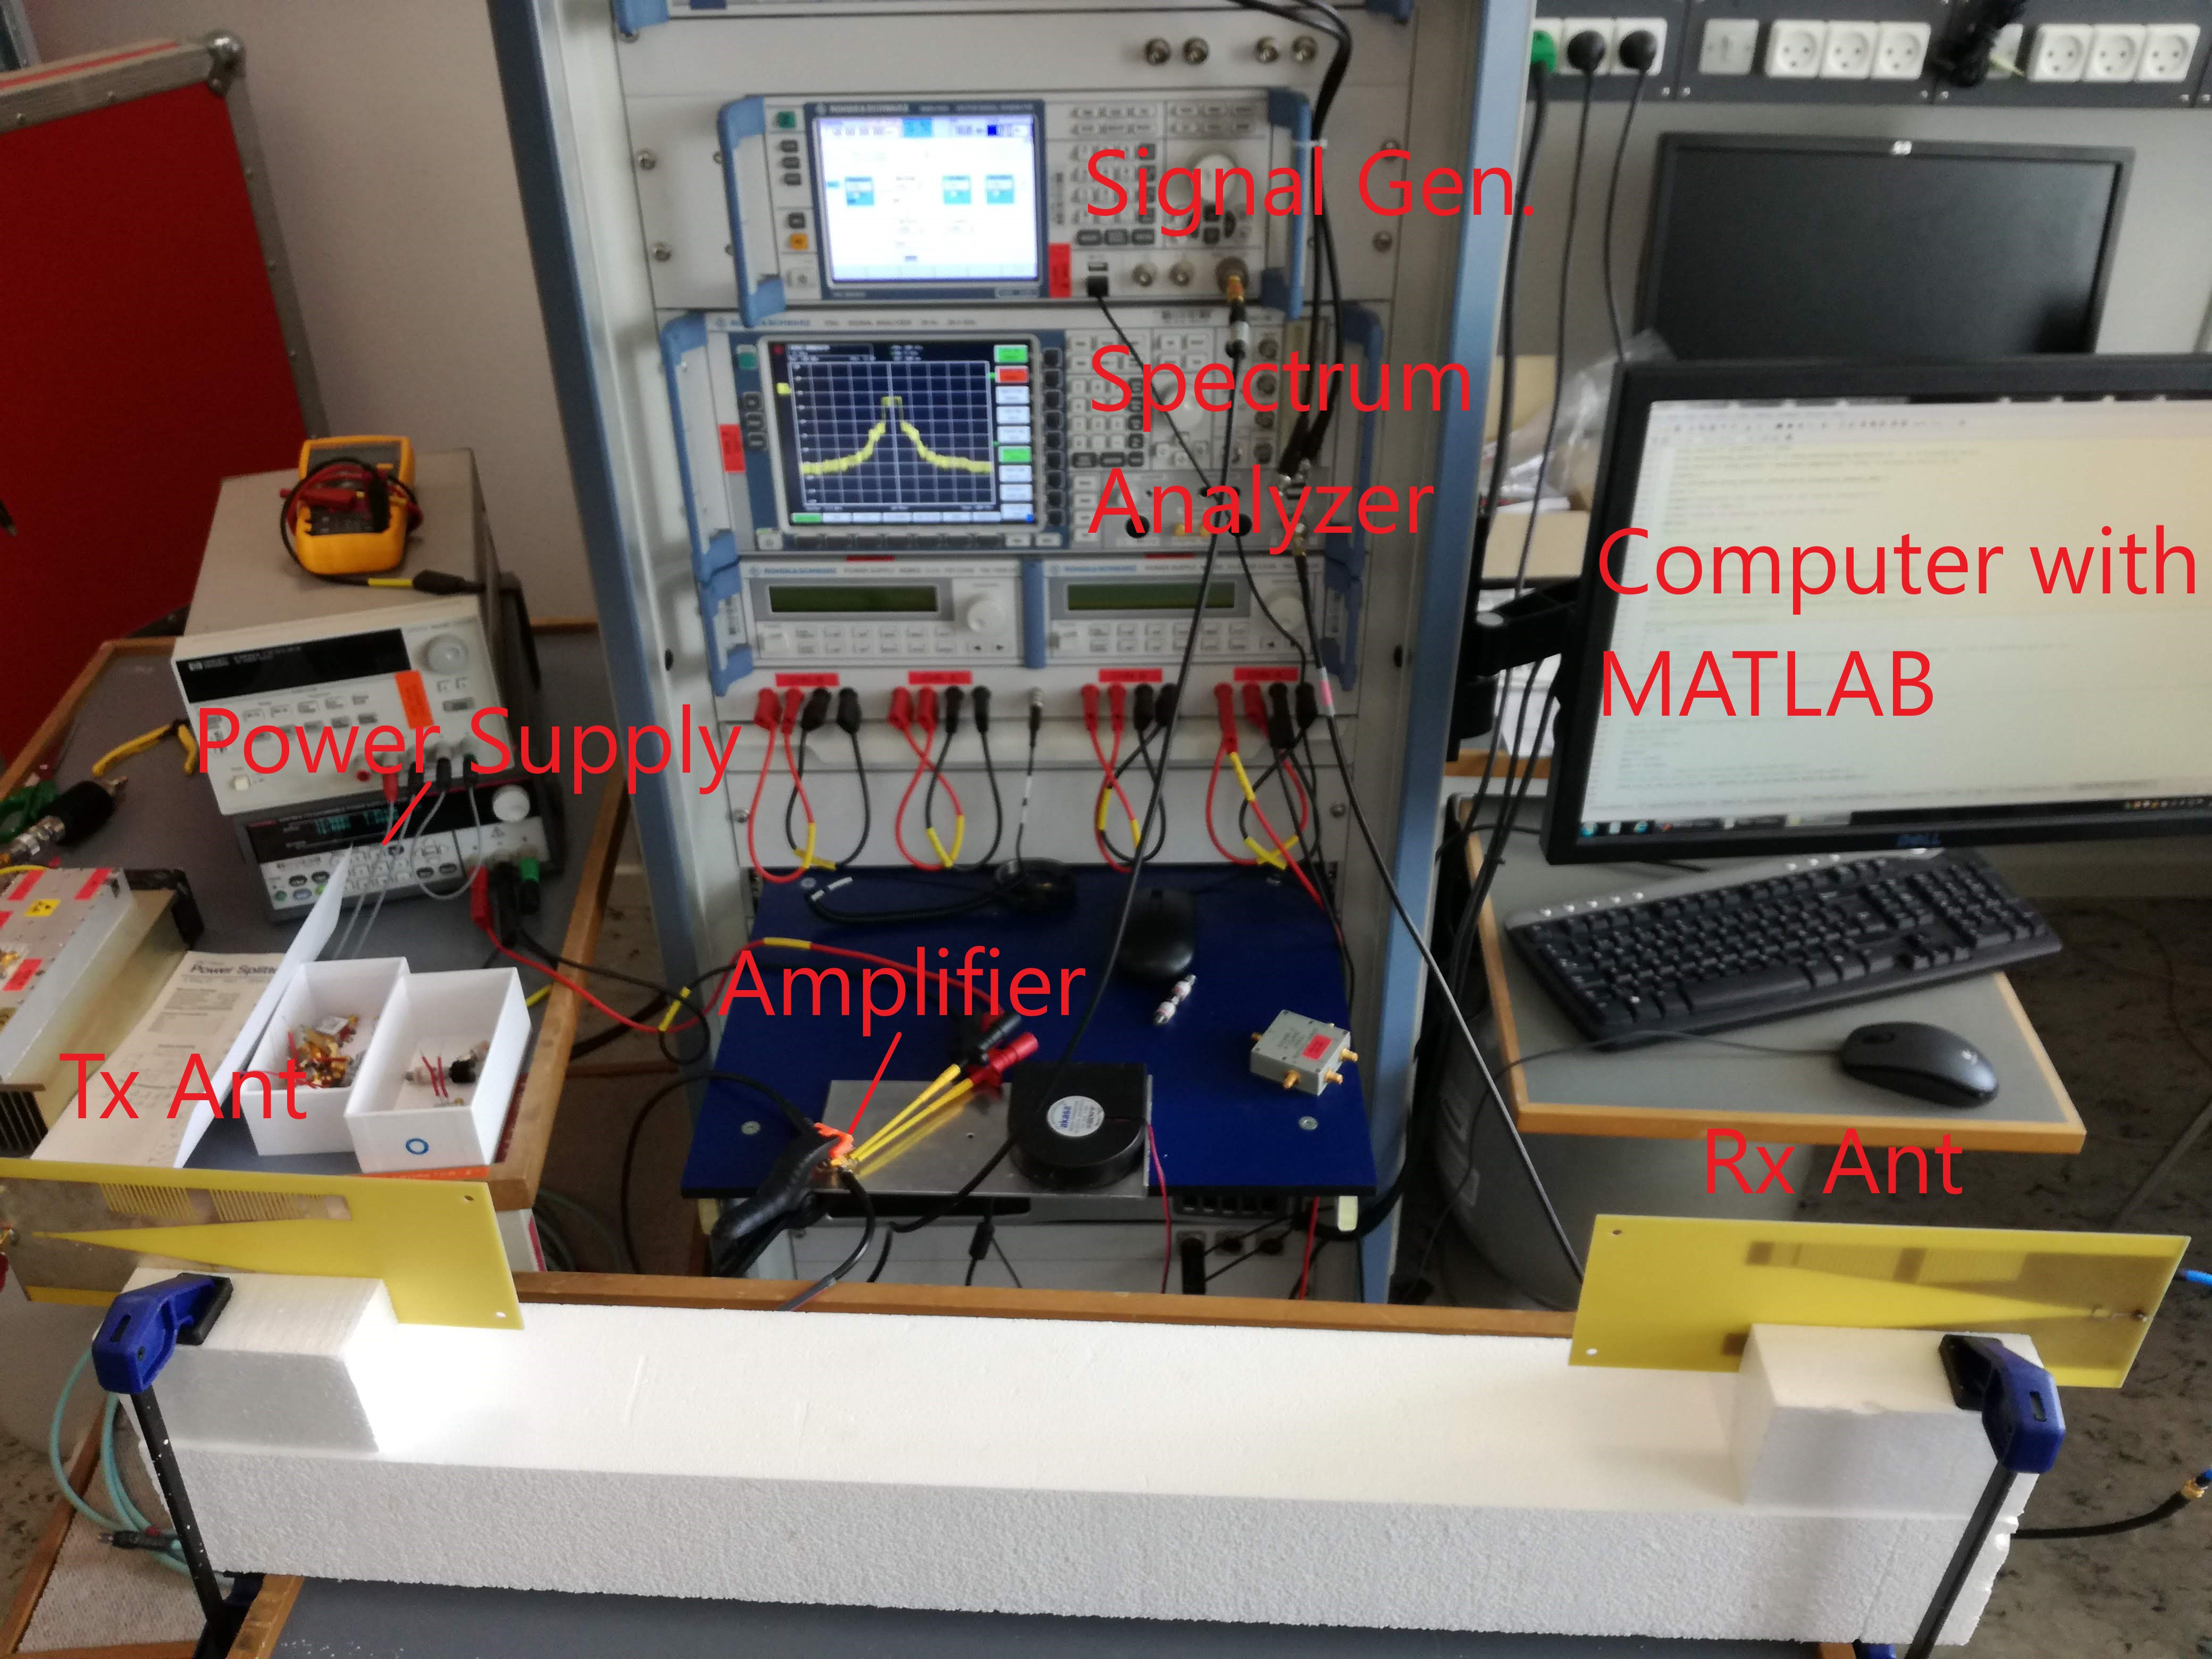
\includegraphics[scale = 0.1]{figures/measurement/measurement_setup.jpg}
\caption{Measurement setup using one transmit antennas}
\label{fig:Meas_setup}
\end{figure} 

\begin{figure}[H]
\centering 
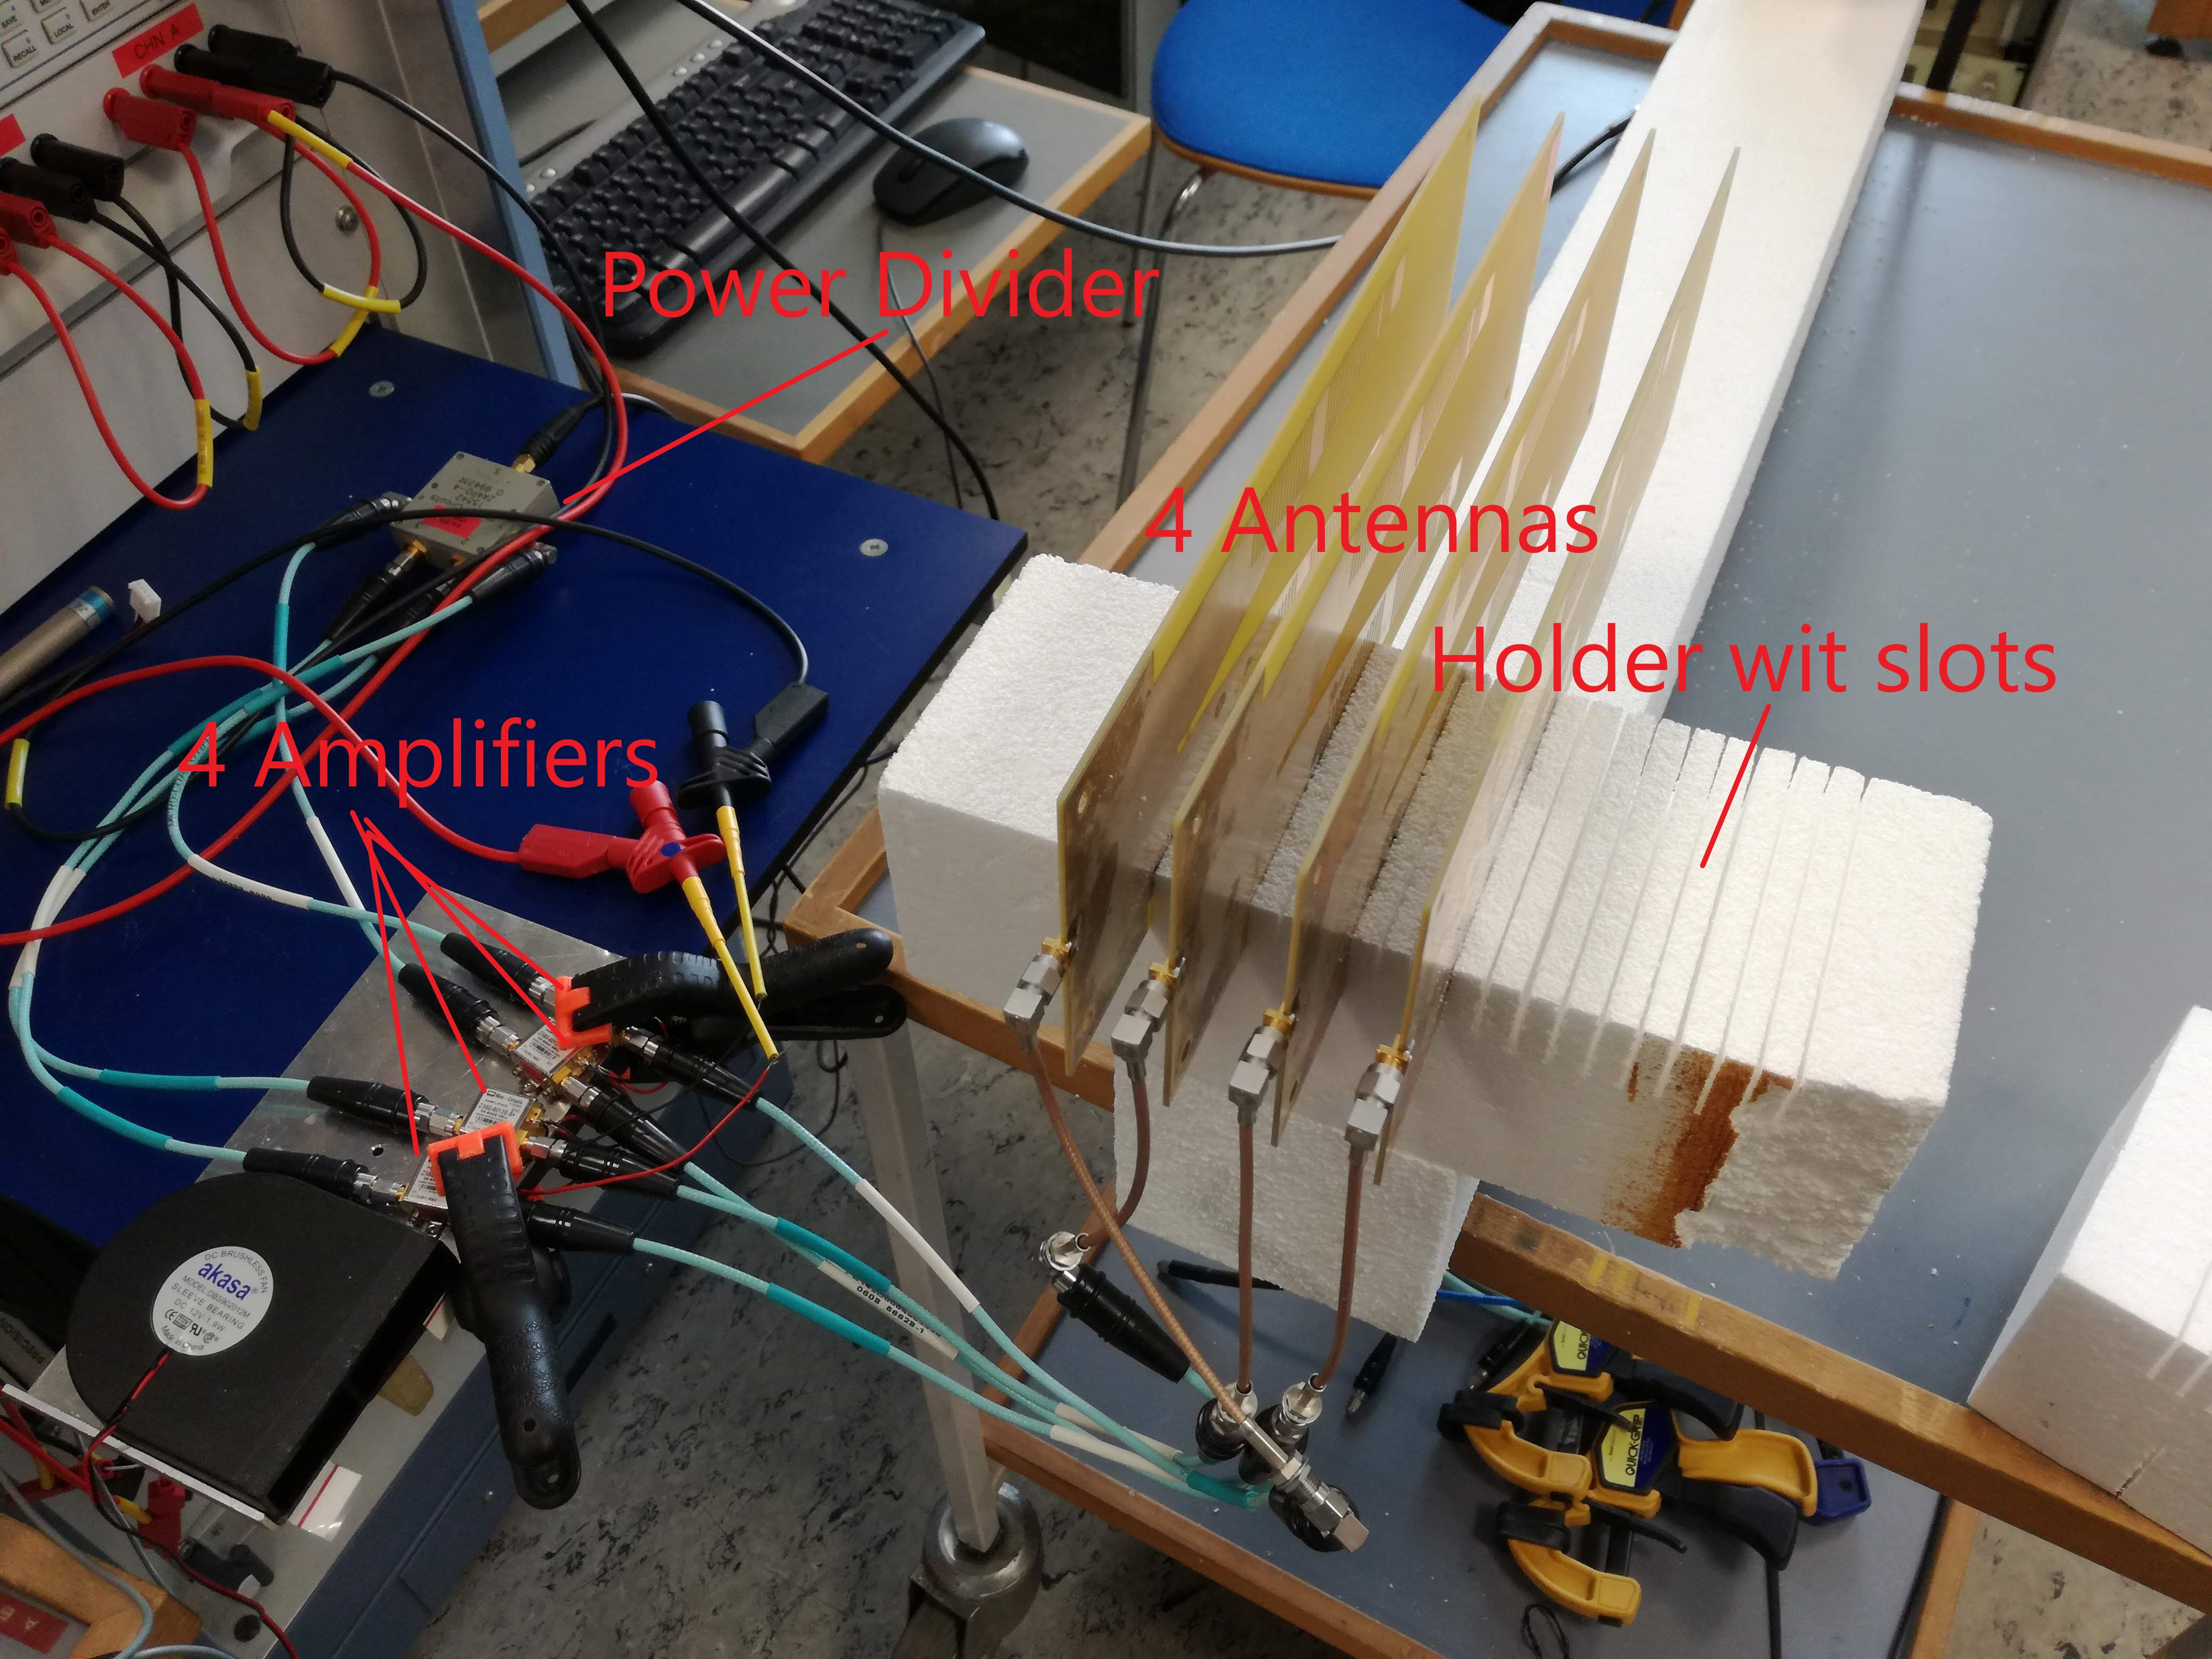
\includegraphics[scale = 0.1]{figures/measurement/measurement_setup_4.jpg}
\caption{Measurement setup using four transmit antennas}
\label{fig:Meas_setup4ant}
\end{figure} 


\subsection{Measurement of AM/AM distortion}\label{ch:meas_amam}
Measurement has been done using the methods described in section \ref{ch_meas_setup}. The results in figure \ref{fig:amam_amp} is a measurement of only the amplifier. It is seen that at an input of -2.5dB the amplifier starts to decrese its gain. This is expected due to the compression point. The mean gain of the amplifier is  measured closly to 13.8dB as expected. It is further seen that the spreading of the signal is highest at low signal levels. When introducing one Tx antenna and one Rx antenna the free space loss must be accounted for. This is done by use of equation \ref{eq:friss_1m} \citep{Balanis2005} which gives 20.5dB in loss. In the measurement 19.5dB was measured, the difference is might caused by the antenna them self, since the used antenna gain is only simulated, and the antenna are spaced relativity close, or it can be reflections from the table or room that are causing the difference. Cable loss and connector loss has been measured and accounted for.  

\begin{equation}\label{eq:friss_1m}
Pathloss(db) = 10*log10(G_r G_t (\frac{4\pi d}{\lambda})^2)=20.5dB
\end{equation}

The measurement using one Tx antenna and one Rx antenna shows that the gain of the system now becomes close to 6dB, this is also expected since the gain of the system is: 

\begin{equation}
G_{system}(dB) = G_{amplifier}+G_{antenna}-Pathloss = 13.85dB + 11.4dB -19.5dB = 5.75dB
\end{equation}

It can be seen from figure \ref{fig:amam_one_ant} that the antenna system makes the AM/AM distortion wider at the compression point, but smaller at lower power levels. In figure \ref{fig:amam01} to \ref{fig:amam06} the results from measurement setup three is shown. The results are made with two transmit antennas and therefore the system gain is increased by 3dB. The results shows small variations due to AM/AM distortion between, but a significant change in AM/AM at compression point in the pre-sentence of two antennas instead of one. Also AM/AM at lower power levels seems to decrease with two antennas compared to one. 

\begin{figure}[H]
  \centering
  \begin{minipage}[b]{0.5\textwidth}
	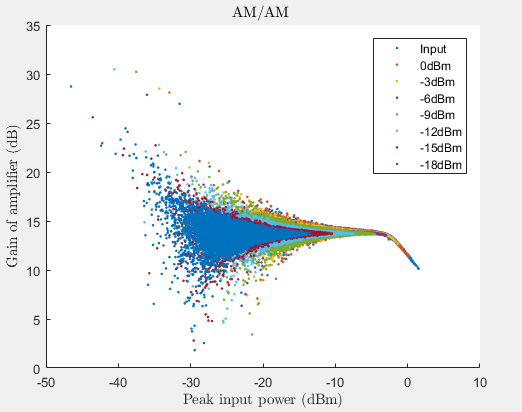
\includegraphics[scale = 0.5]{figures/measurement/two_antenna/amplifier_amam.png}
	\caption{AM/AM distortion at amplifier}
    \label{fig:amam_amp}
  \end{minipage}
  \hfill
  \begin{minipage}[b]{0.4\textwidth}
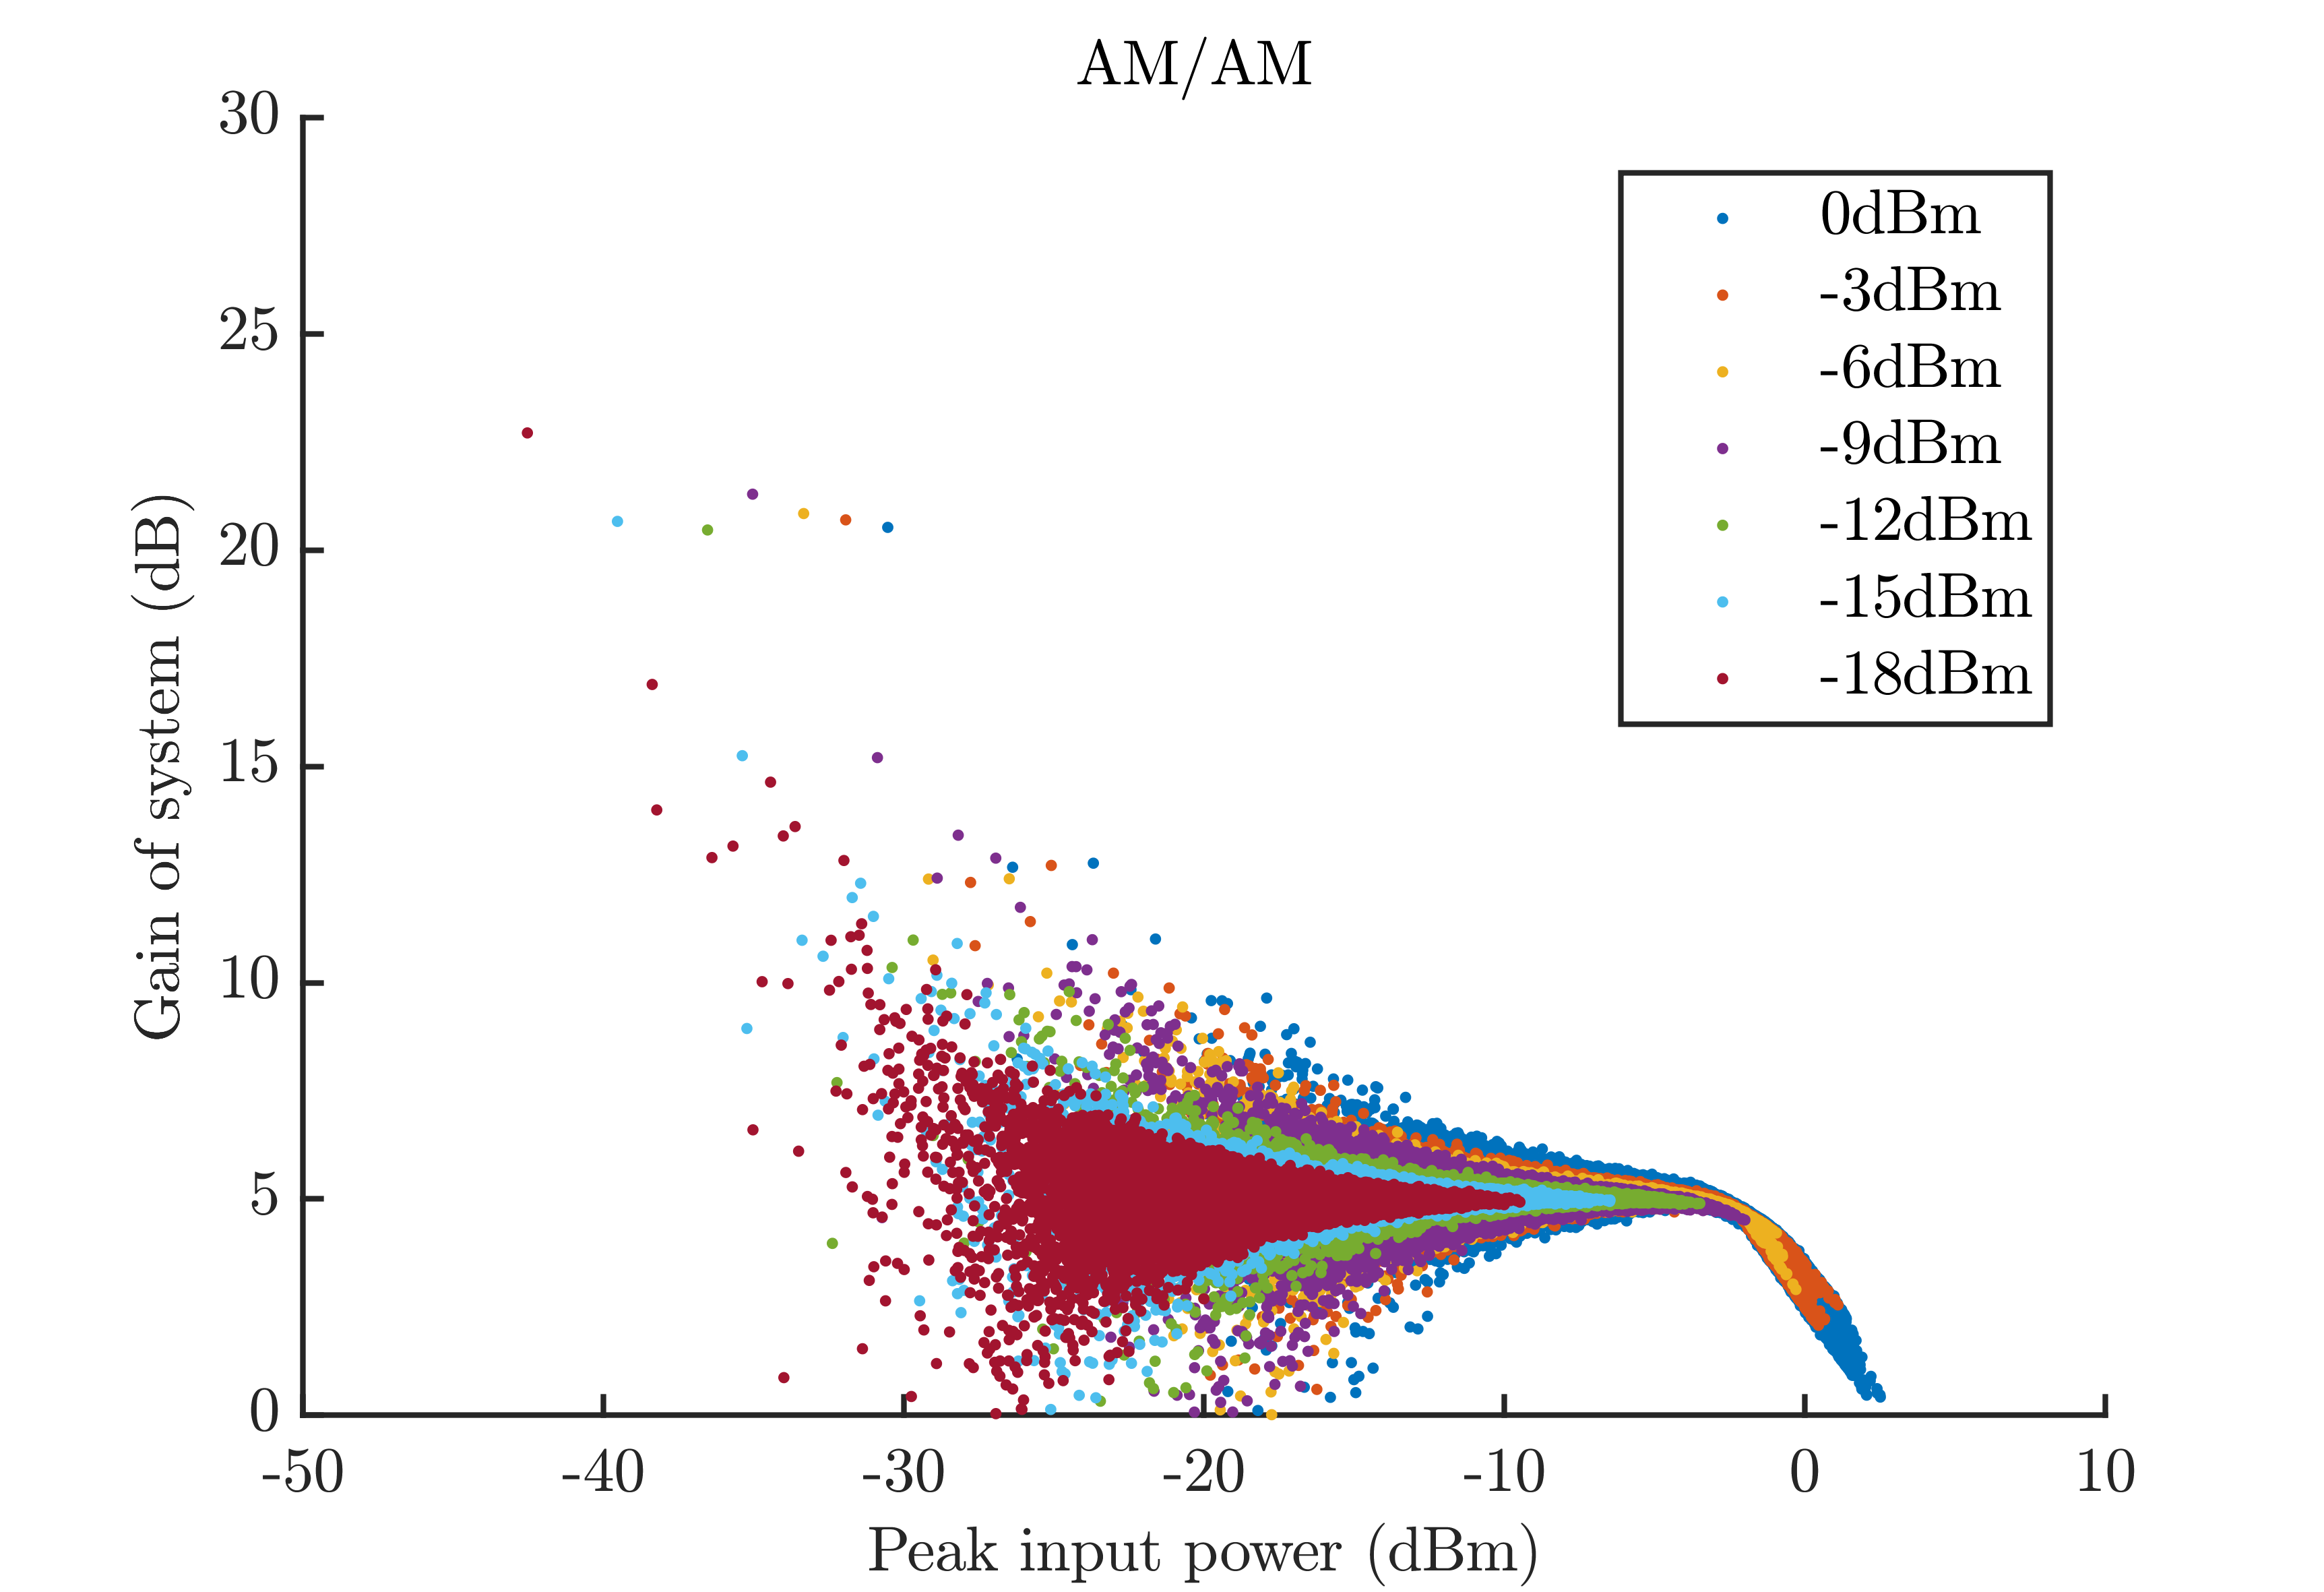
\includegraphics[scale = 0.5]{figures/measurement/two_antenna/one_ant_amam.png}
\caption{AM/AM distortion using one transmit antenna}
    \label{fig:amam_one_ant}
  \end{minipage}
\end{figure}

\subsubsection{Two transmit antenna}

\begin{figure}[H]
  \centering
  \begin{minipage}[b]{0.5\textwidth}
	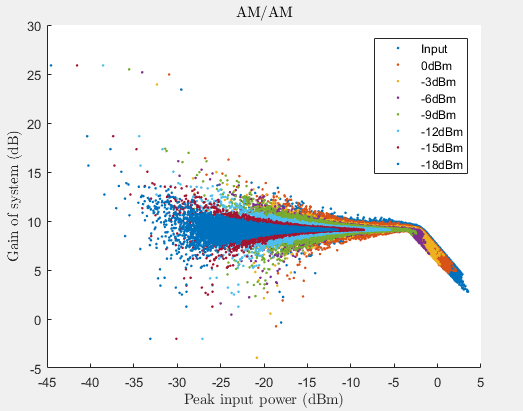
\includegraphics[scale = 0.5]{figures/measurement/two_antenna/amam_01.png}
	\caption{AM/AM distortion at 0.1 $\lambda$ spacing between two antennas}
    \label{fig:amam01}
  \end{minipage}
  \hfill
  \begin{minipage}[b]{0.4\textwidth}
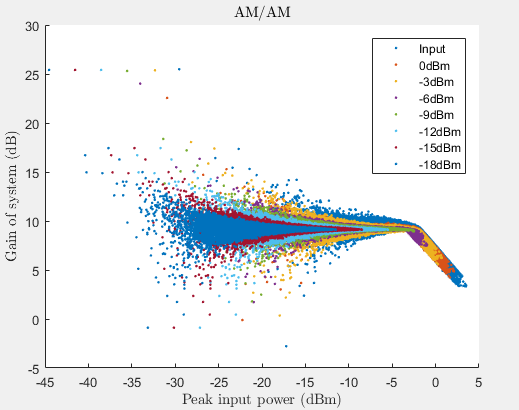
\includegraphics[scale = 0.5]{figures/measurement/two_antenna/amam_02.png}
\caption{AM/AM distortion at 0.2 $\lambda$ spacing between two antennas}
    \label{fig:amam02}
  \end{minipage}
\end{figure}

\begin{figure}[H]
  \centering
  \begin{minipage}[b]{0.5\textwidth}
	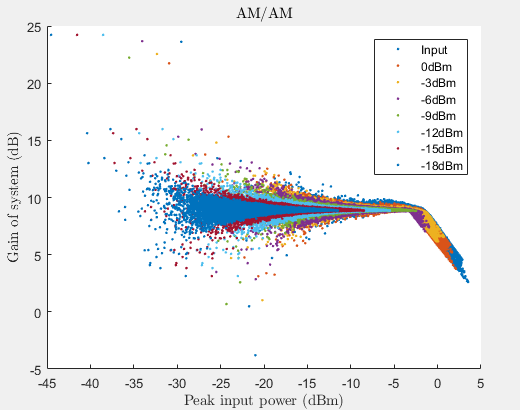
\includegraphics[scale = 0.5]{figures/measurement/two_antenna/amam_03.png}
	\caption{AM/AM distortion at 0.3 $\lambda$ spacing between two antennas}
    \label{fig:amam03}
  \end{minipage}
  \hfill
  \begin{minipage}[b]{0.4\textwidth}
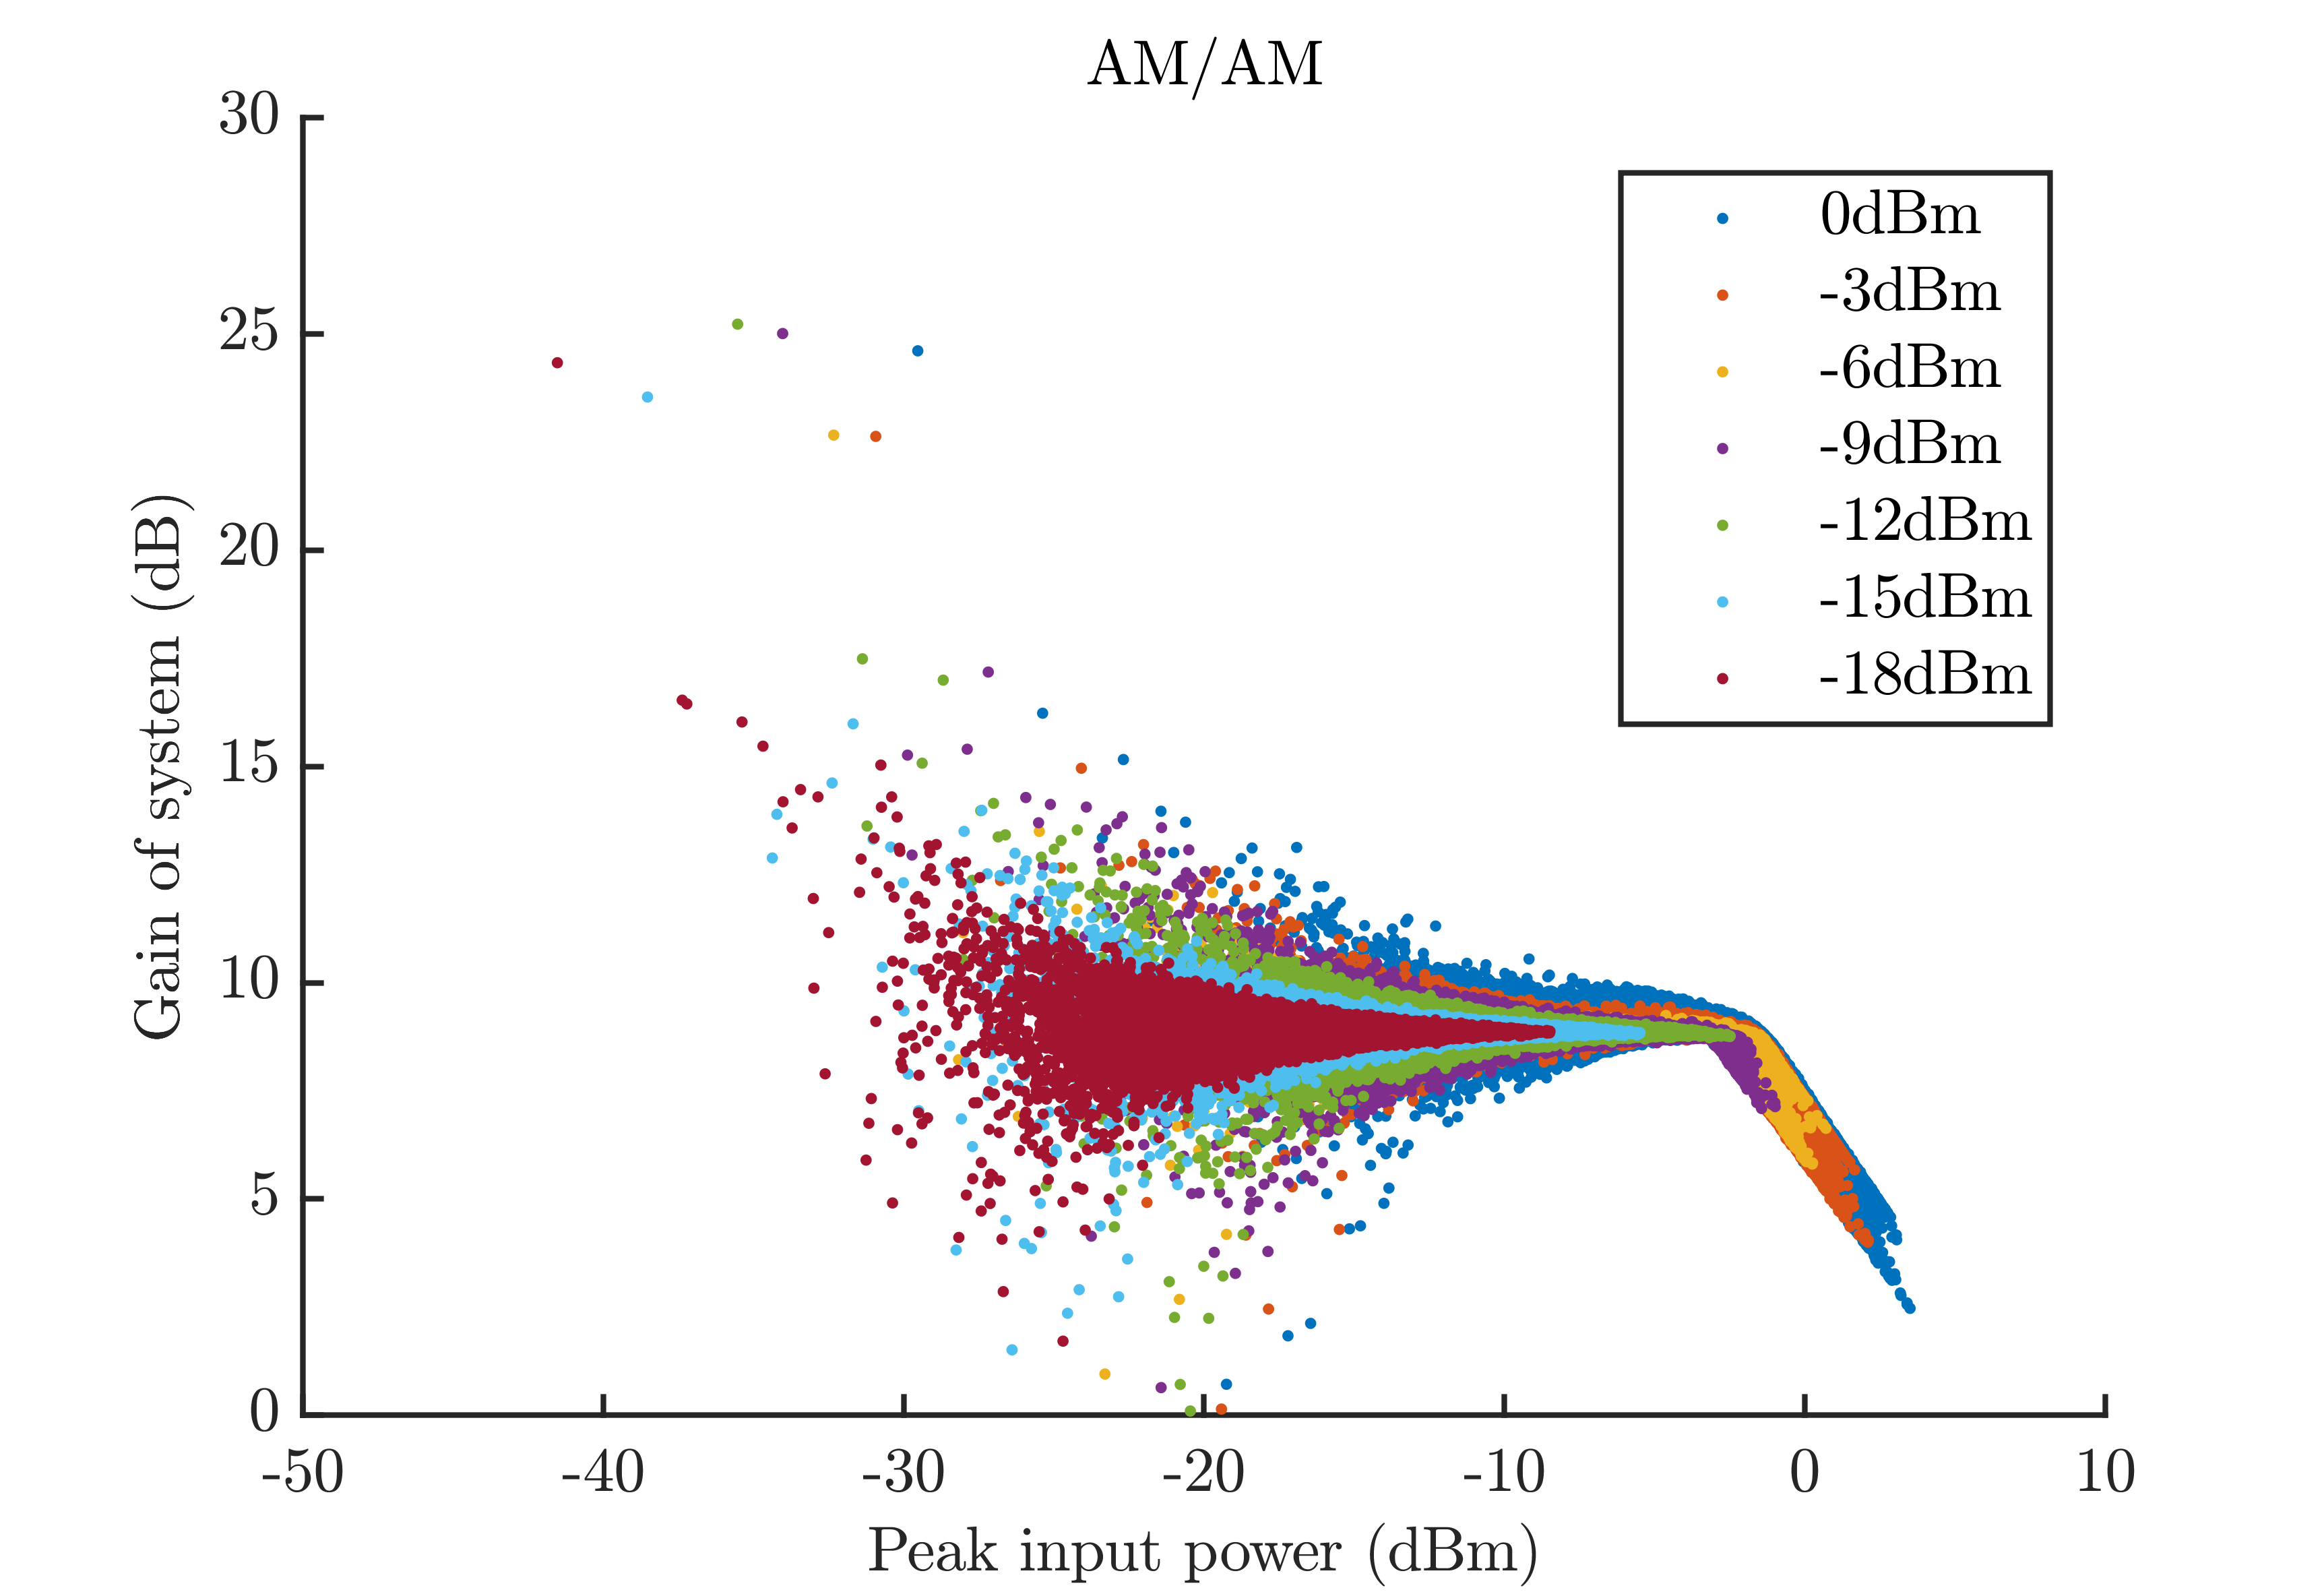
\includegraphics[scale = 0.5]{figures/measurement/two_antenna/amam_04.png}
\caption{AM/AM distortion at 0.4 $\lambda$ spacing between two antennas}
    \label{fig:amam04}
  \end{minipage}
\end{figure}

\begin{figure}[H]
  \centering
  \begin{minipage}[b]{0.5\textwidth}
	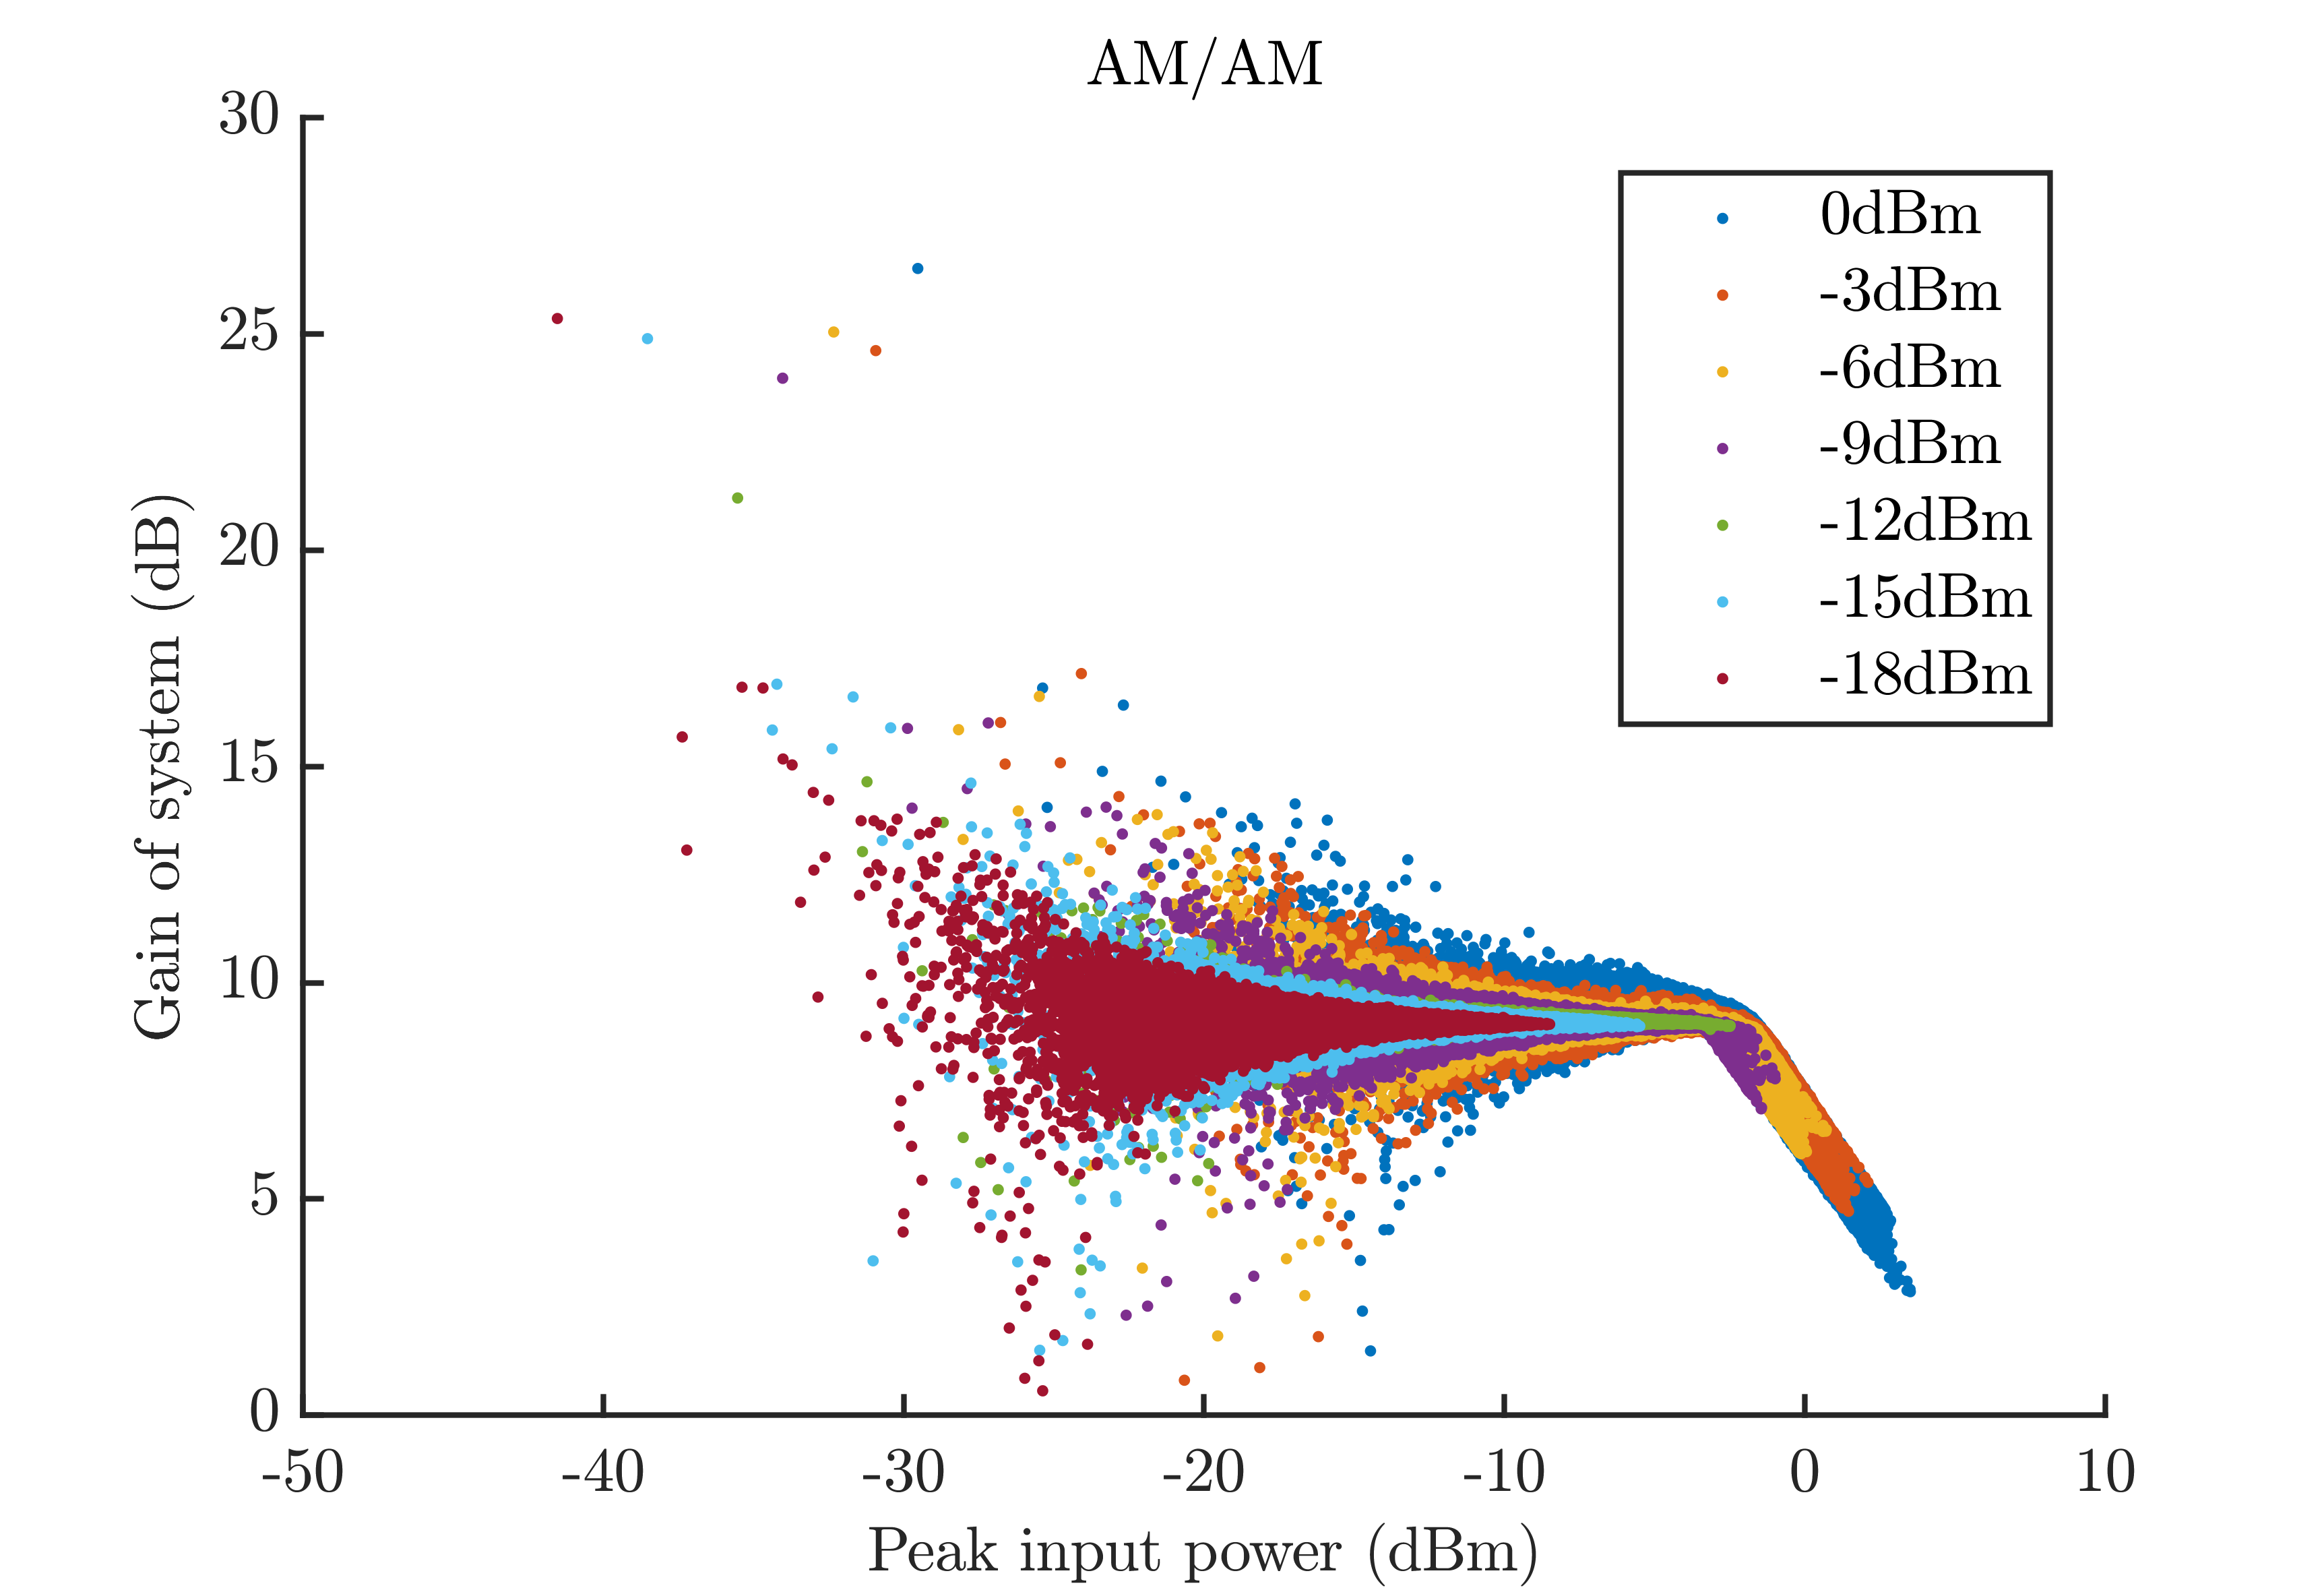
\includegraphics[scale = 0.5]{figures/measurement/two_antenna/amam_05.png}
	\caption{AM/AM distortion at 0.5 $\lambda$ spacing between two antennas}
    \label{fig:amam05}
  \end{minipage}
  \hfill
  \begin{minipage}[b]{0.4\textwidth}
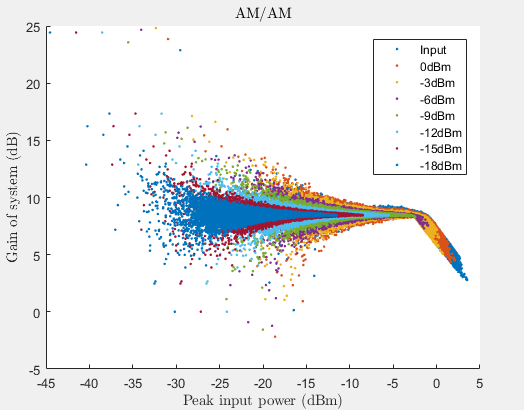
\includegraphics[scale = 0.5]{figures/measurement/two_antenna/amam_06.png}
\caption{AM/AM distortion at 0.6 $\lambda$ spacing between two antennas}
    \label{fig:amam06}
  \end{minipage}
\end{figure}

\subsubsection{Four transmit antenna}

\begin{figure}[H]
  \centering
  \begin{minipage}[b]{0.5\textwidth}
	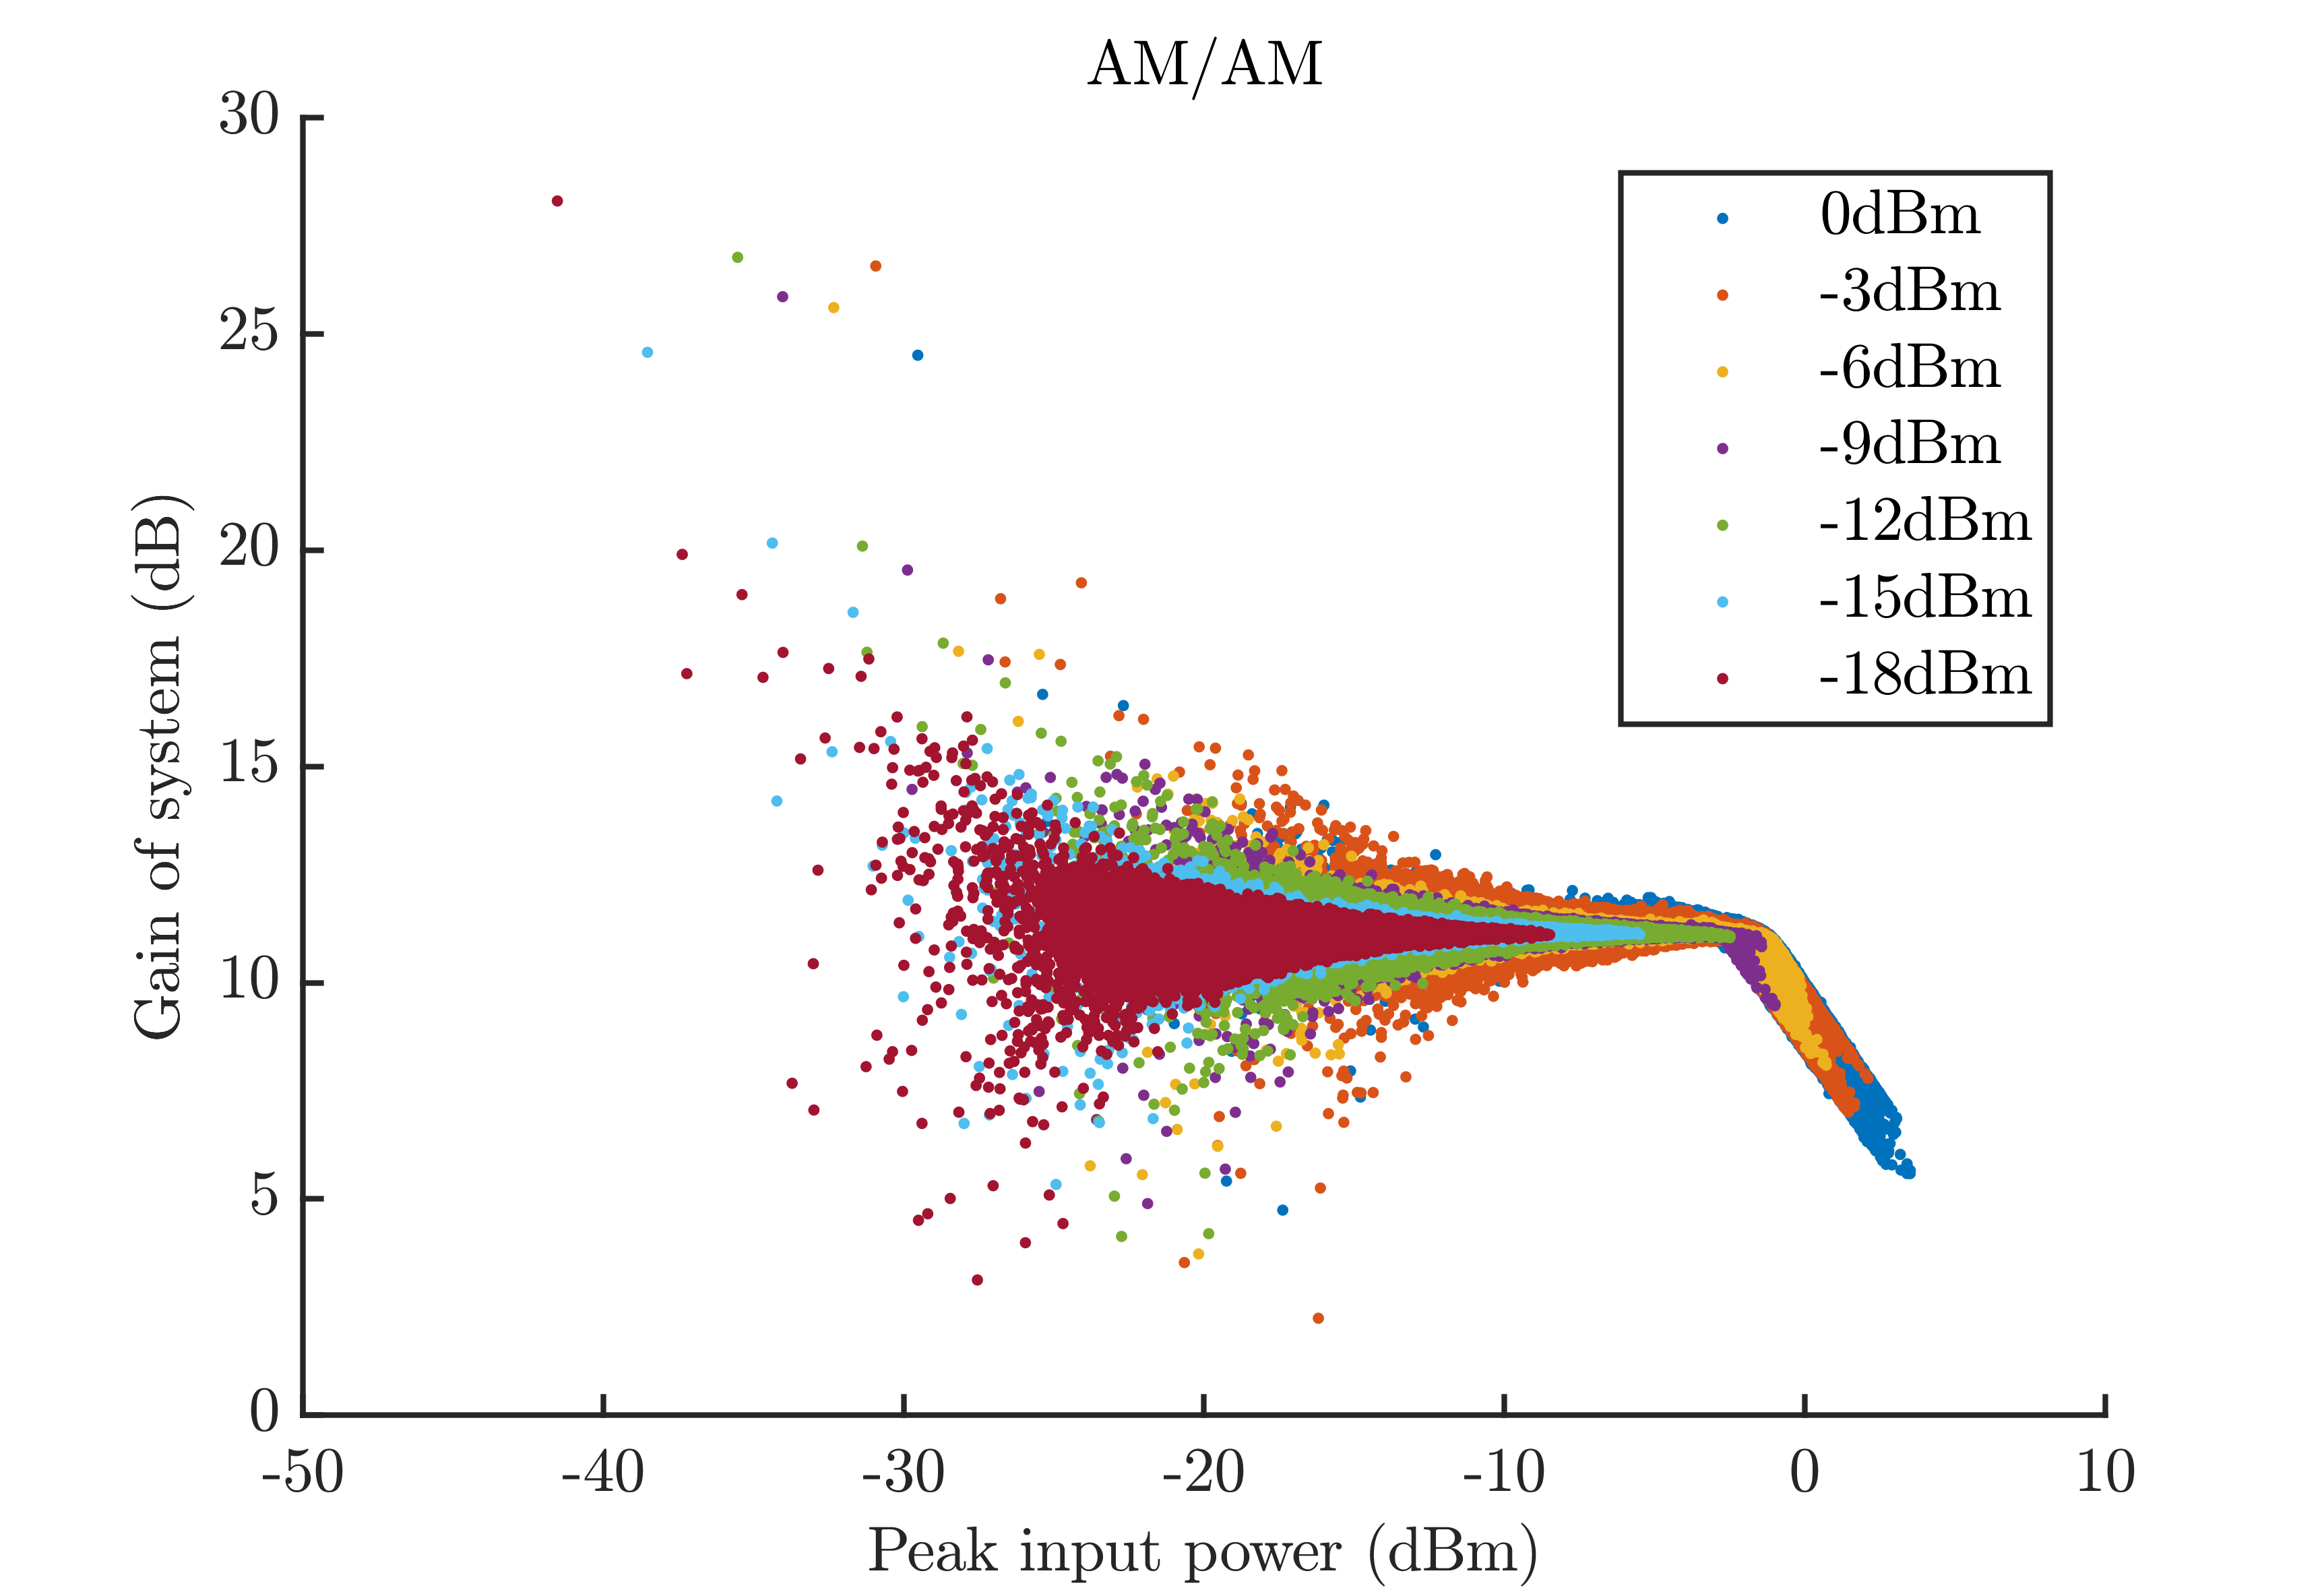
\includegraphics[scale = 0.5]{figures/measurement/four_antenna/amam_0p1.png}
	\caption{AM/AM distortion at 0.1 $\lambda$ spacing between four antennas}
    \label{fig:amam01_4}
  \end{minipage}
  \hfill
  \begin{minipage}[b]{0.4\textwidth}
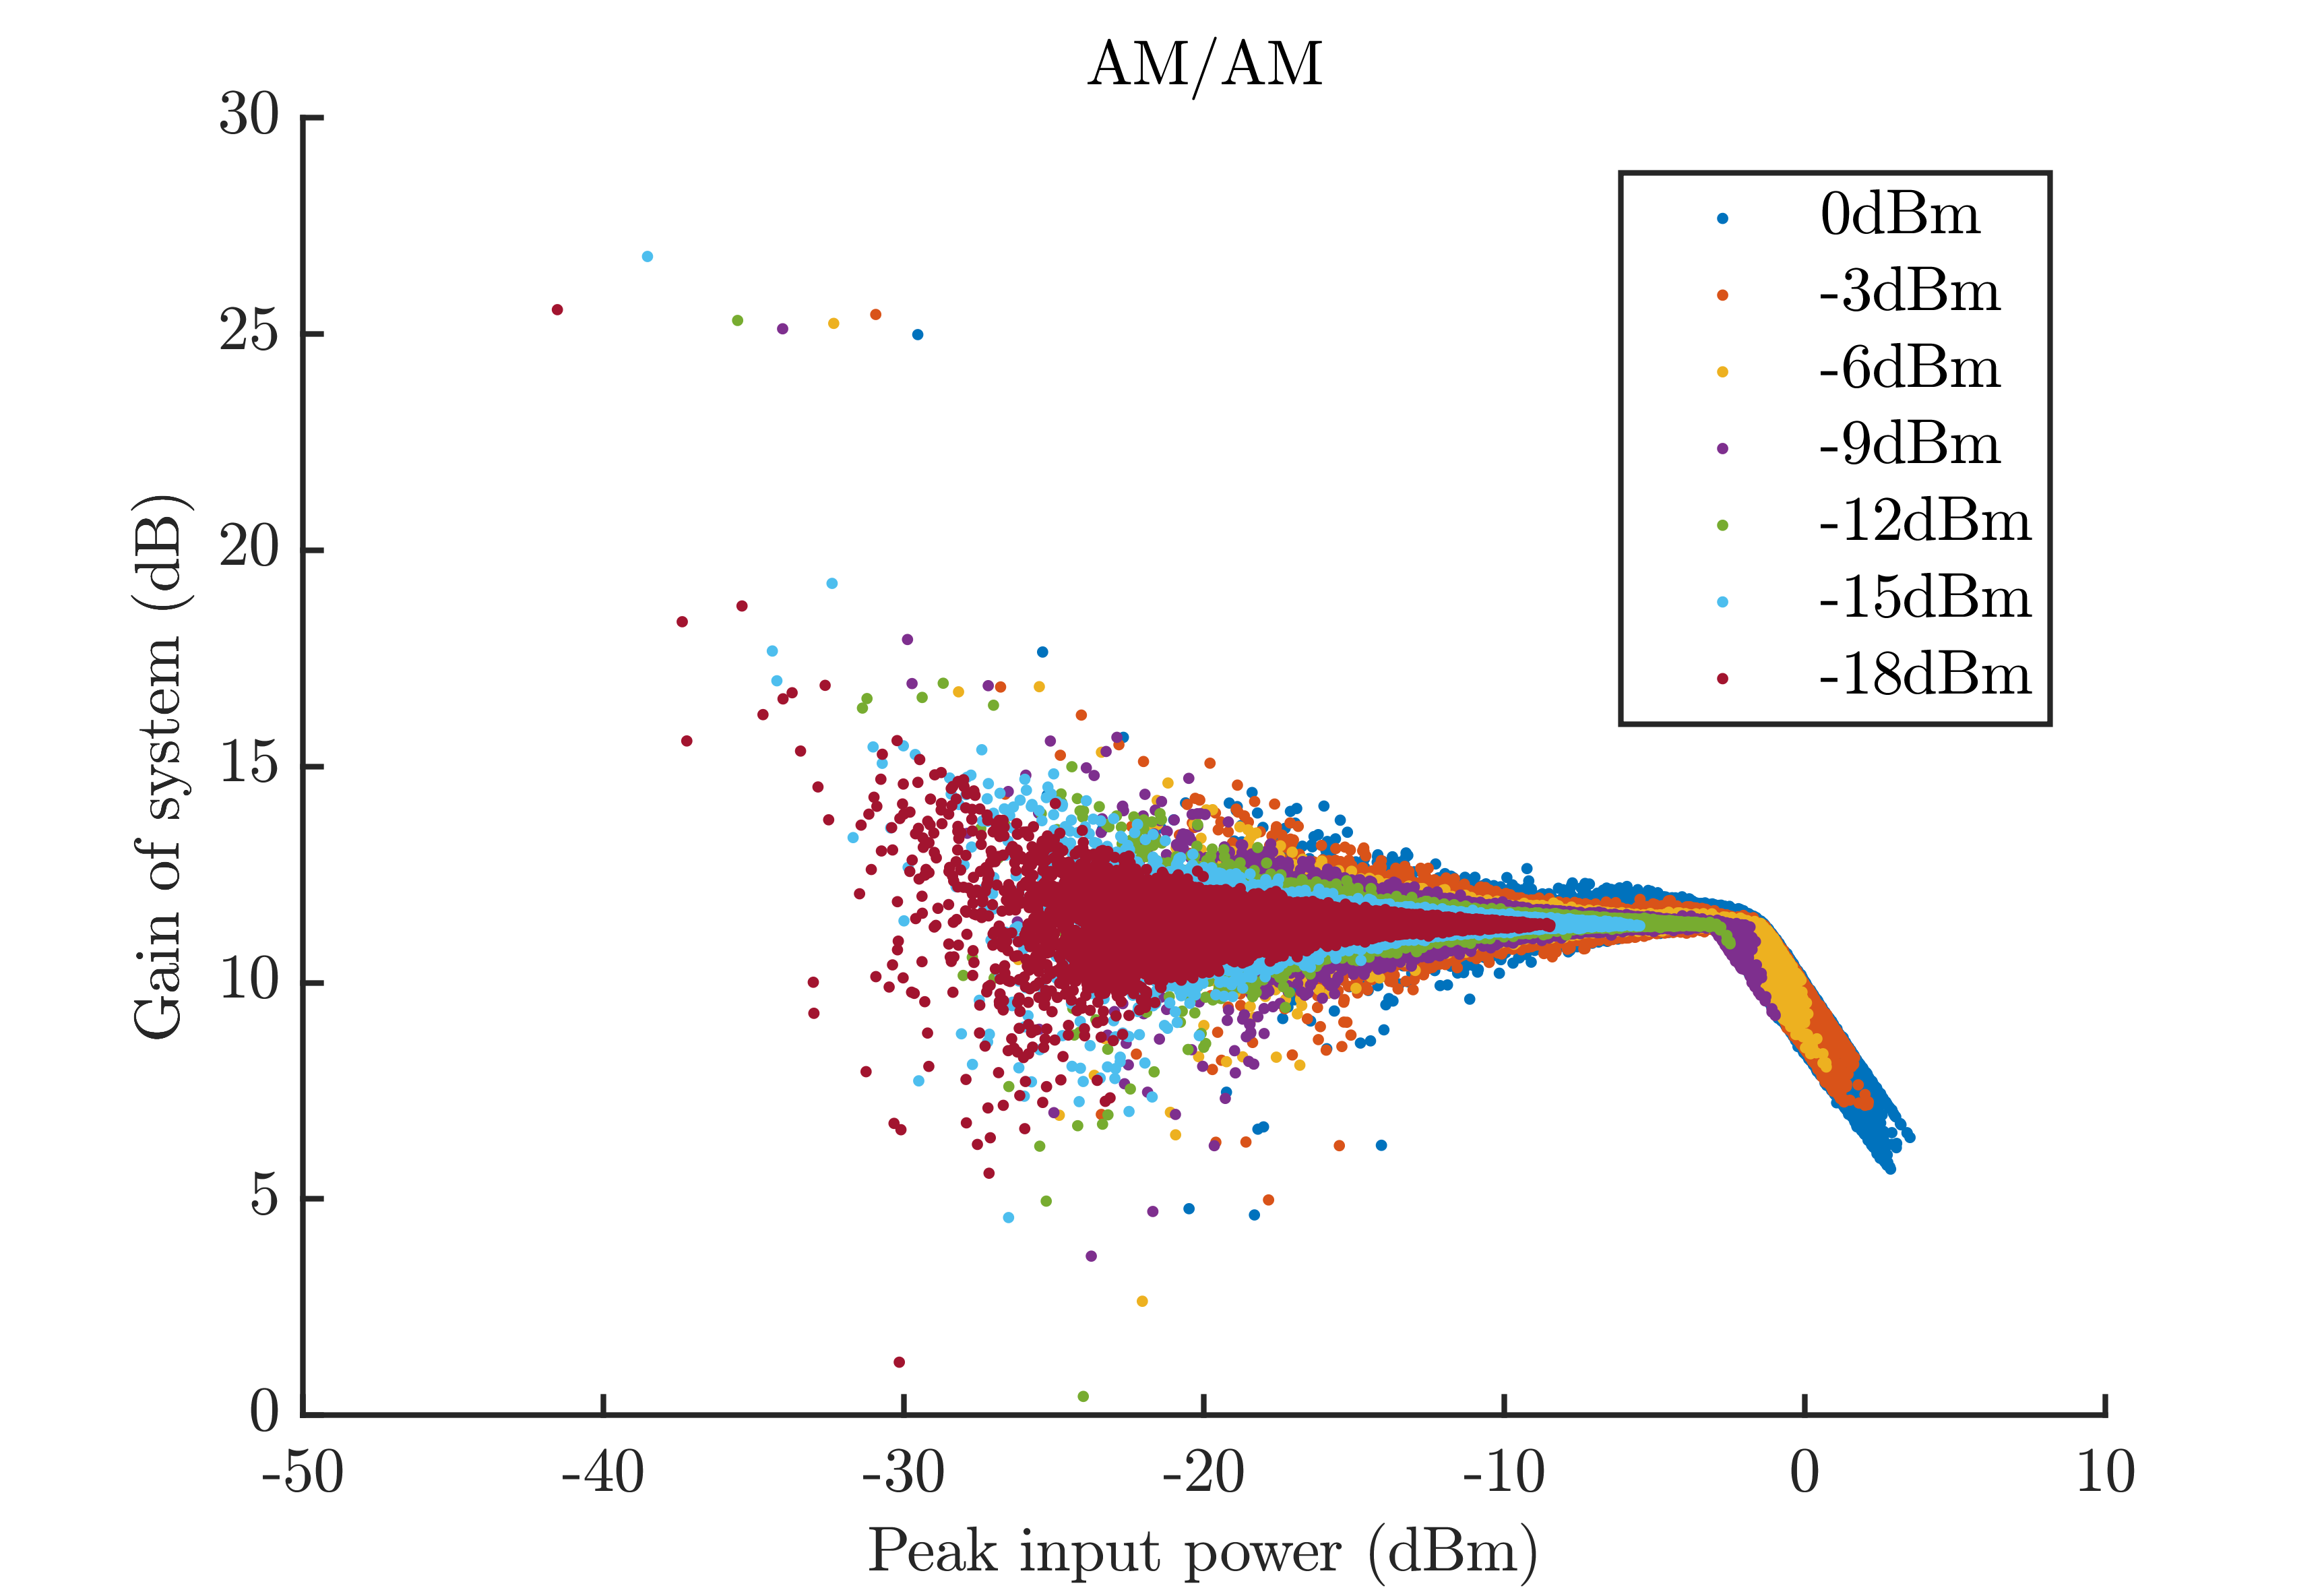
\includegraphics[scale = 0.5]{figures/measurement/four_antenna/amam_0p2.png}
\caption{AM/AM distortion at 0.2 $\lambda$ spacing between four antennas}
    \label{fig:amam02_4}
  \end{minipage}
\end{figure}

\begin{figure}[H]
  \centering
  \begin{minipage}[b]{0.5\textwidth}
	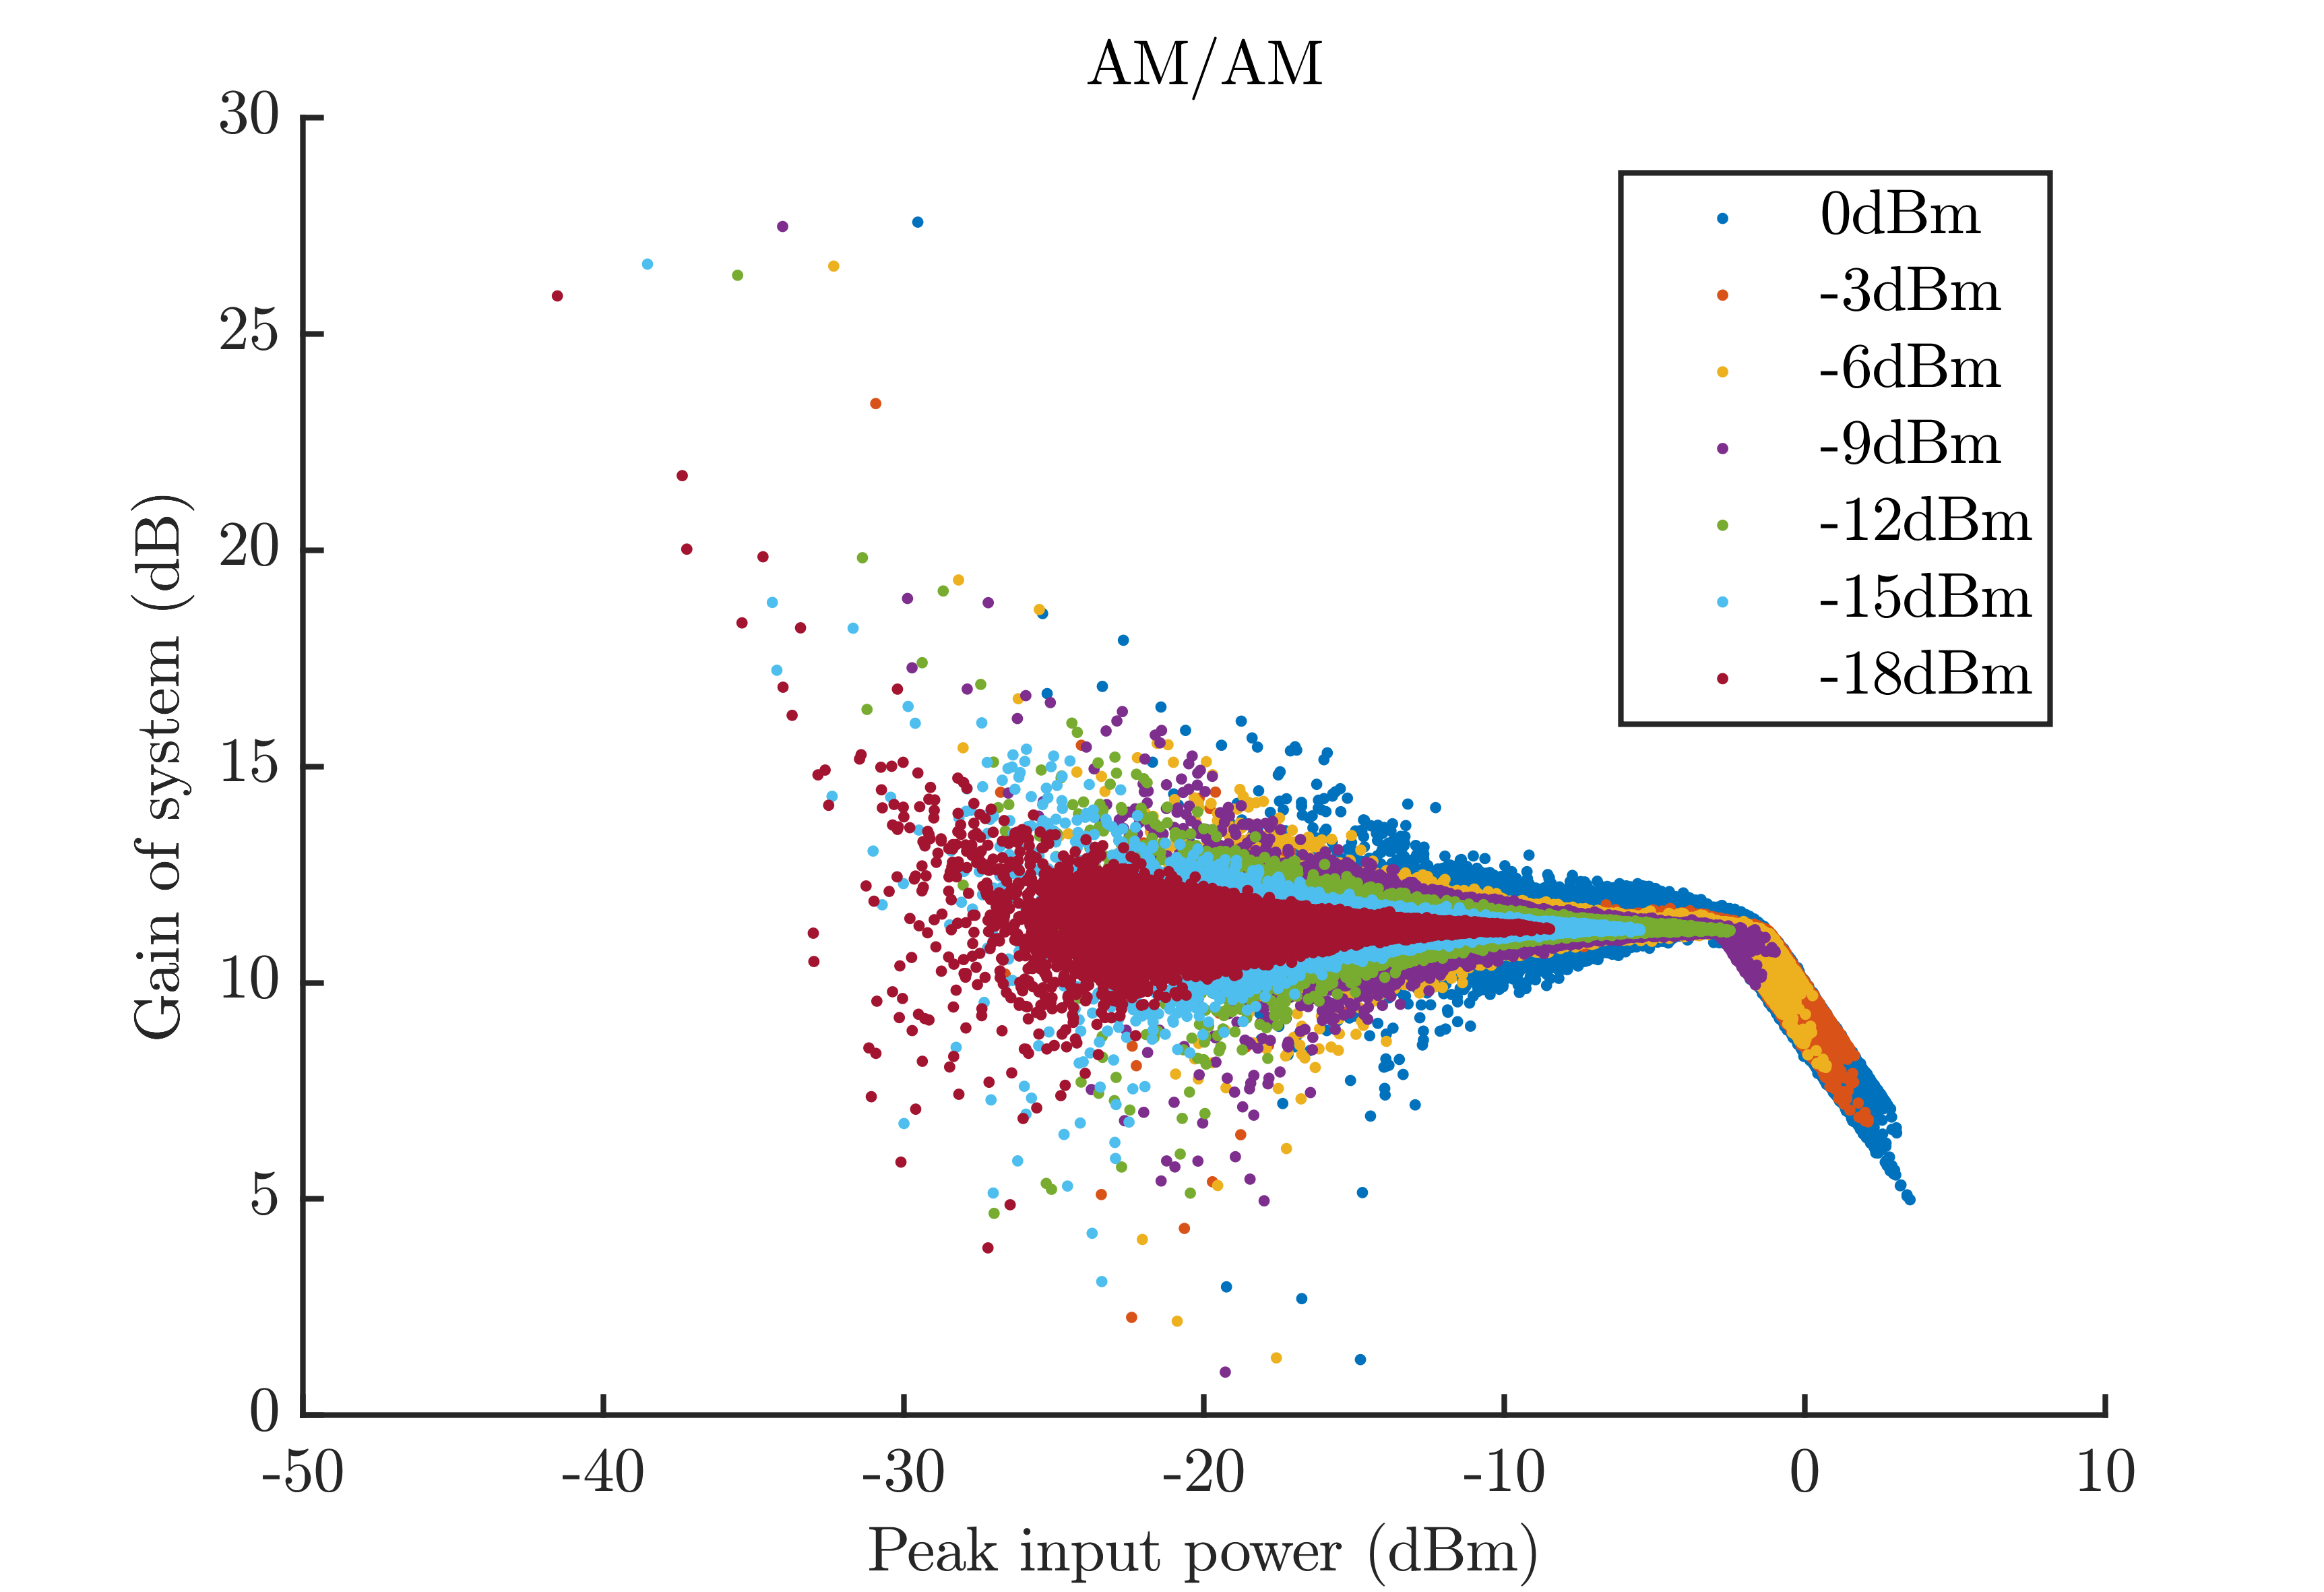
\includegraphics[scale = 0.5]{figures/measurement/four_antenna/amam_0p3.png}
	\caption{AM/AM distortion at 0.3 $\lambda$ spacing between four antennas}
    \label{fig:amam03_4}
  \end{minipage}
  \hfill
  \begin{minipage}[b]{0.4\textwidth}
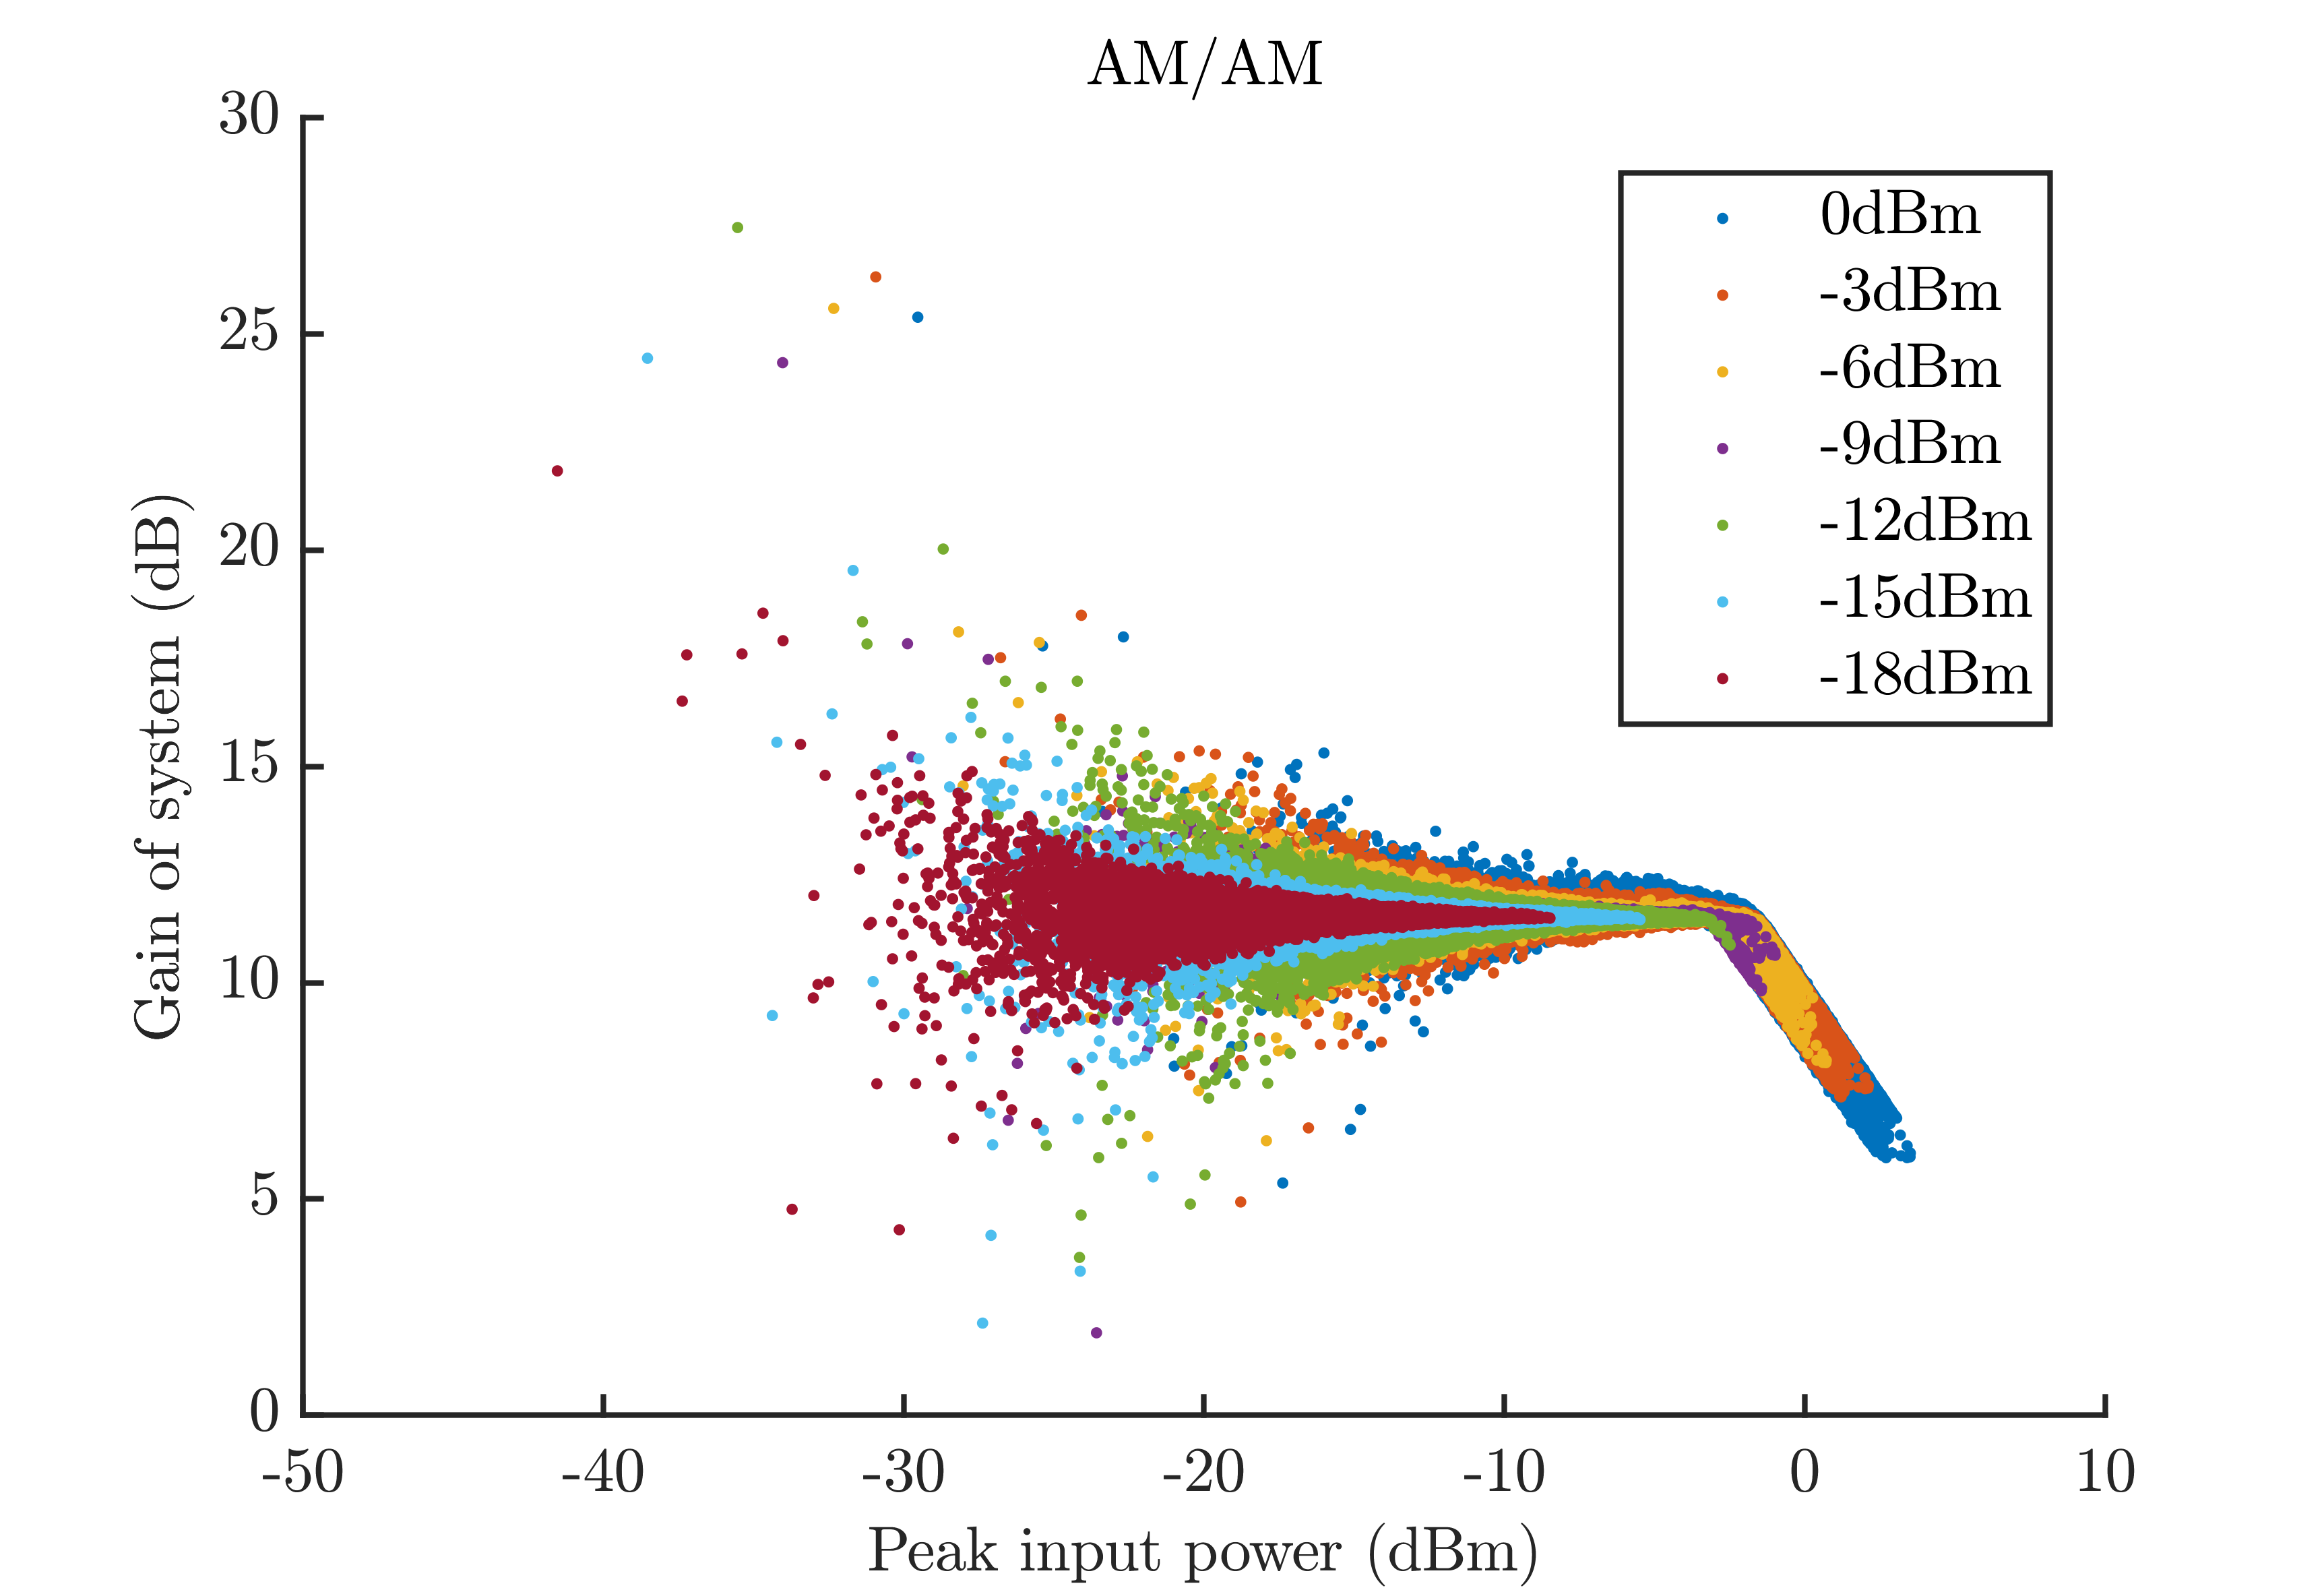
\includegraphics[scale = 0.5]{figures/measurement/four_antenna/amam_0p4.png}
\caption{AM/AM distortion at 0.4 $\lambda$ spacing between four antennas}
    \label{fig:amam04_4}
  \end{minipage}
\end{figure}

\begin{figure}[H]
  \centering
  \begin{minipage}[b]{0.5\textwidth}
	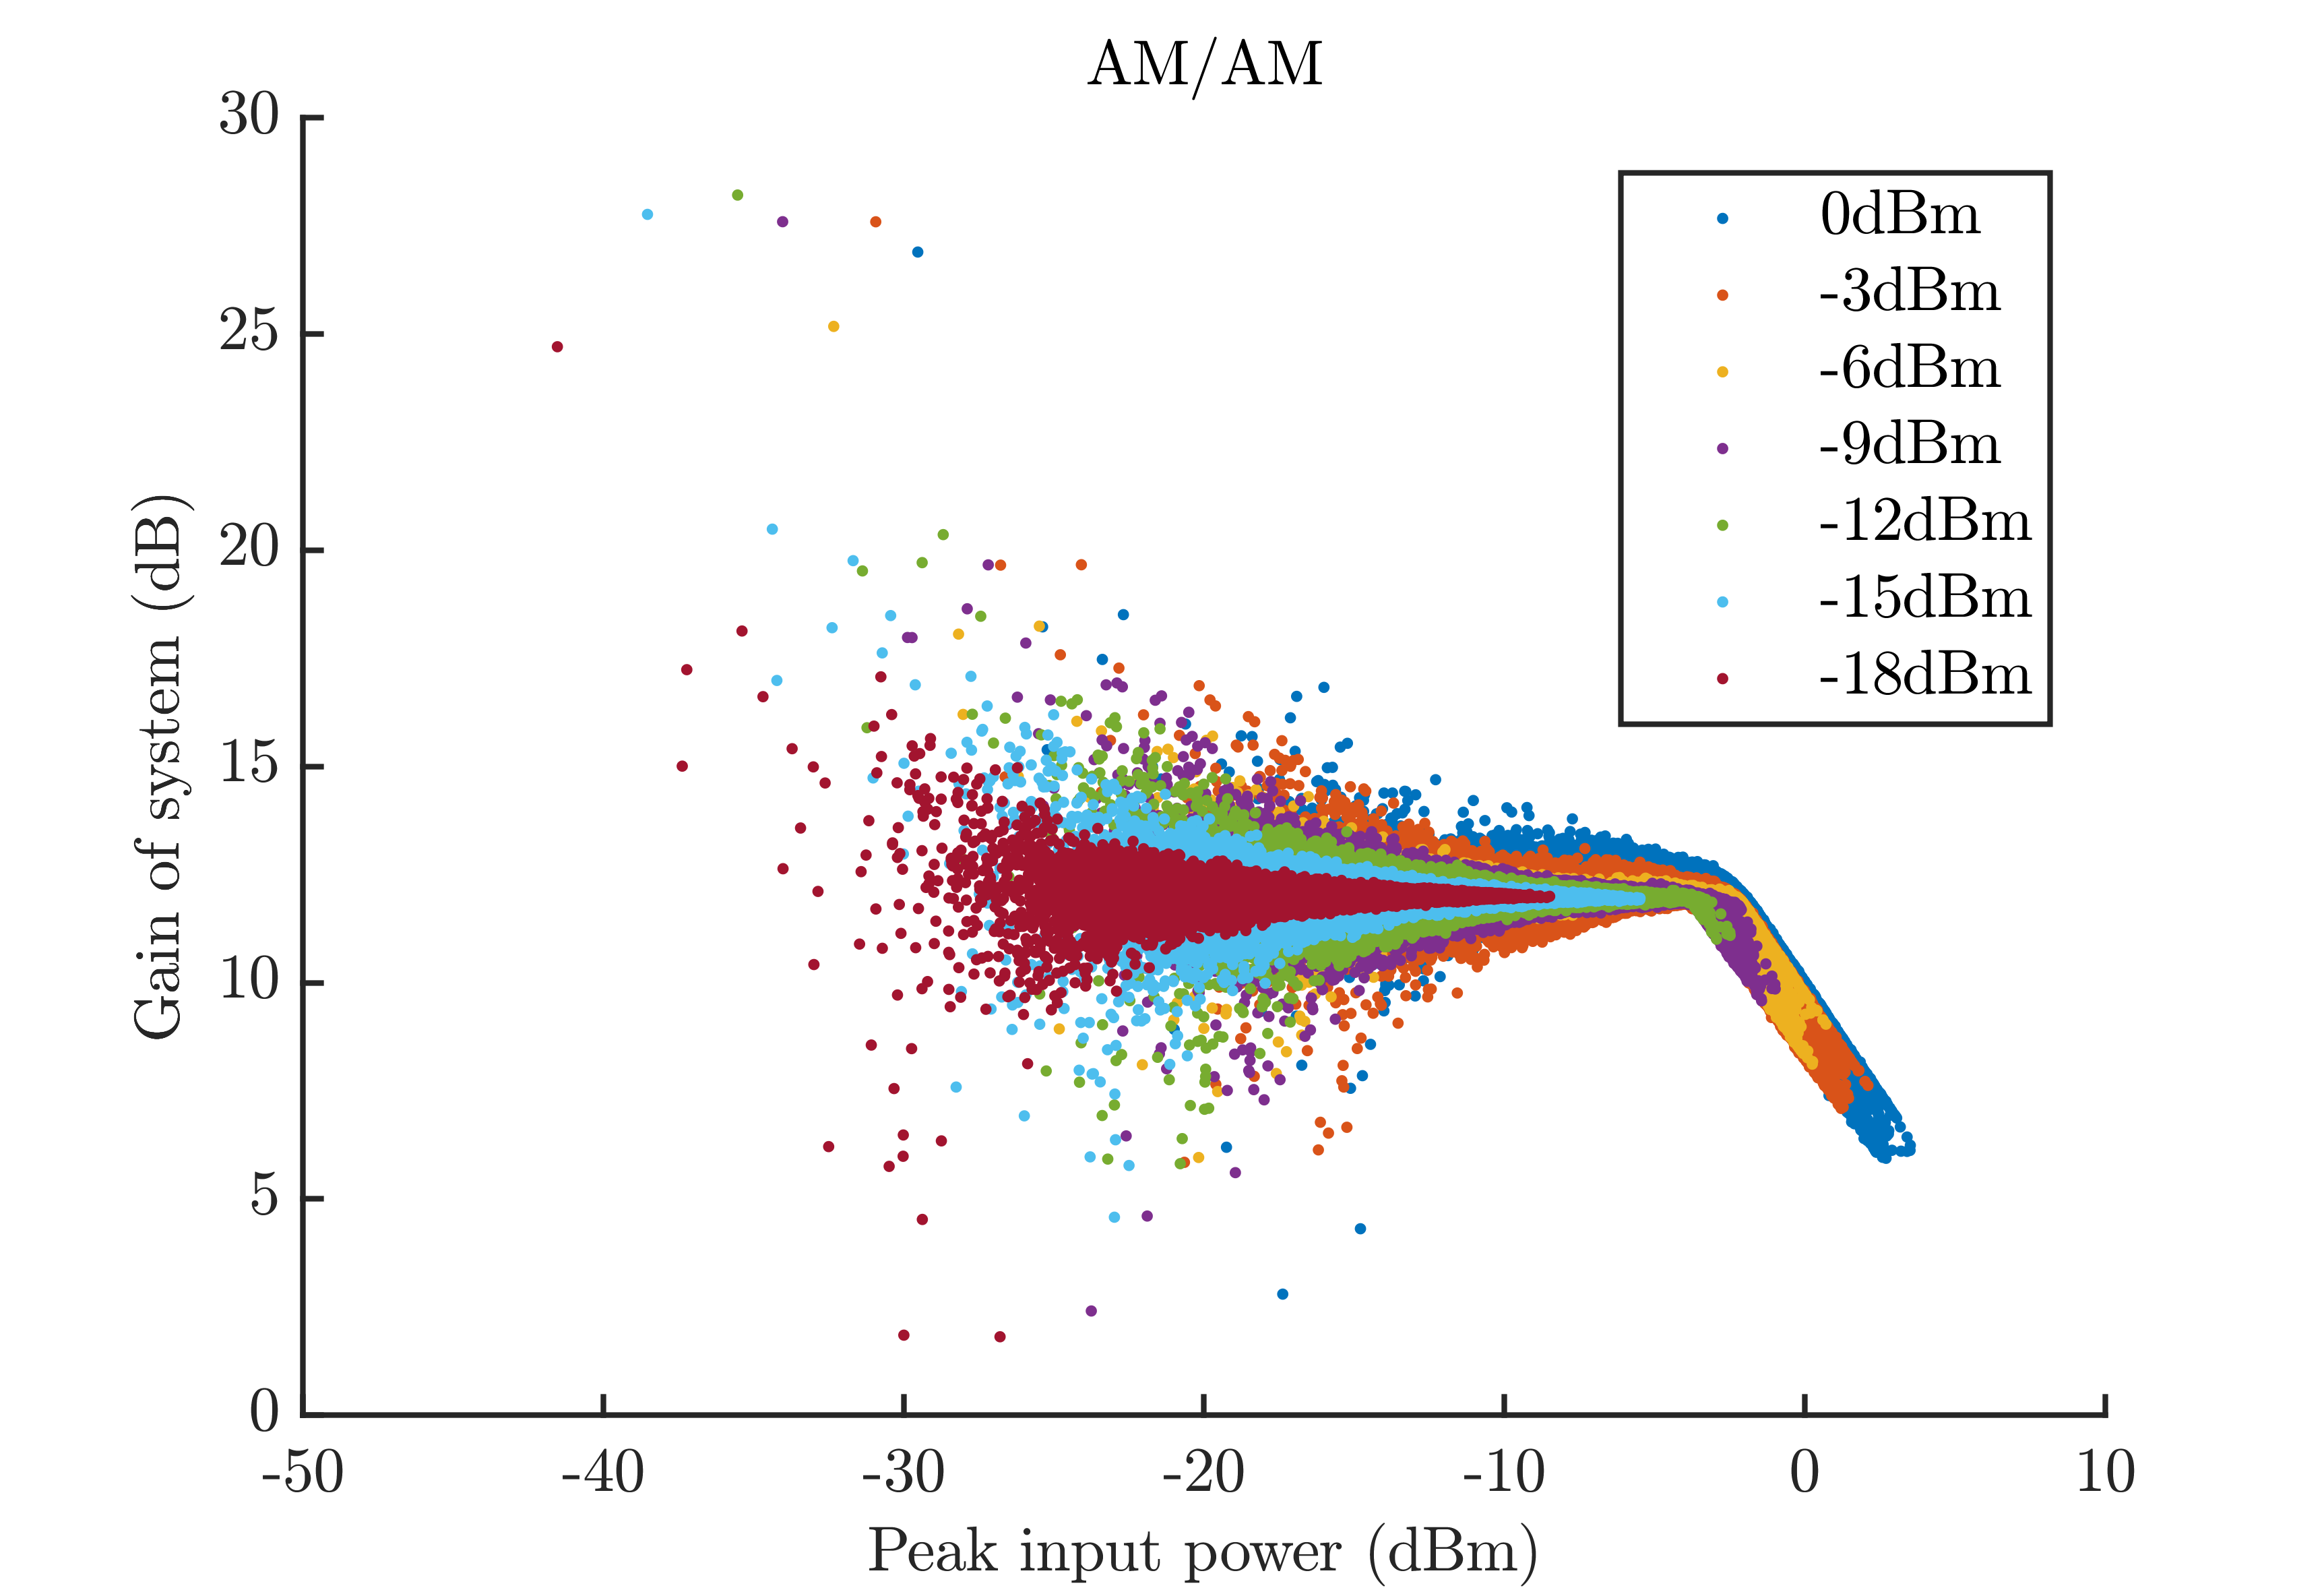
\includegraphics[scale = 0.5]{figures/measurement/four_antenna/amam_0p5.png}
	\caption{AM/AM distortion at 0.5 $\lambda$ spacing between four antennas}
    \label{fig:amam05_4}
  \end{minipage}
  \hfill
  \begin{minipage}[b]{0.4\textwidth}
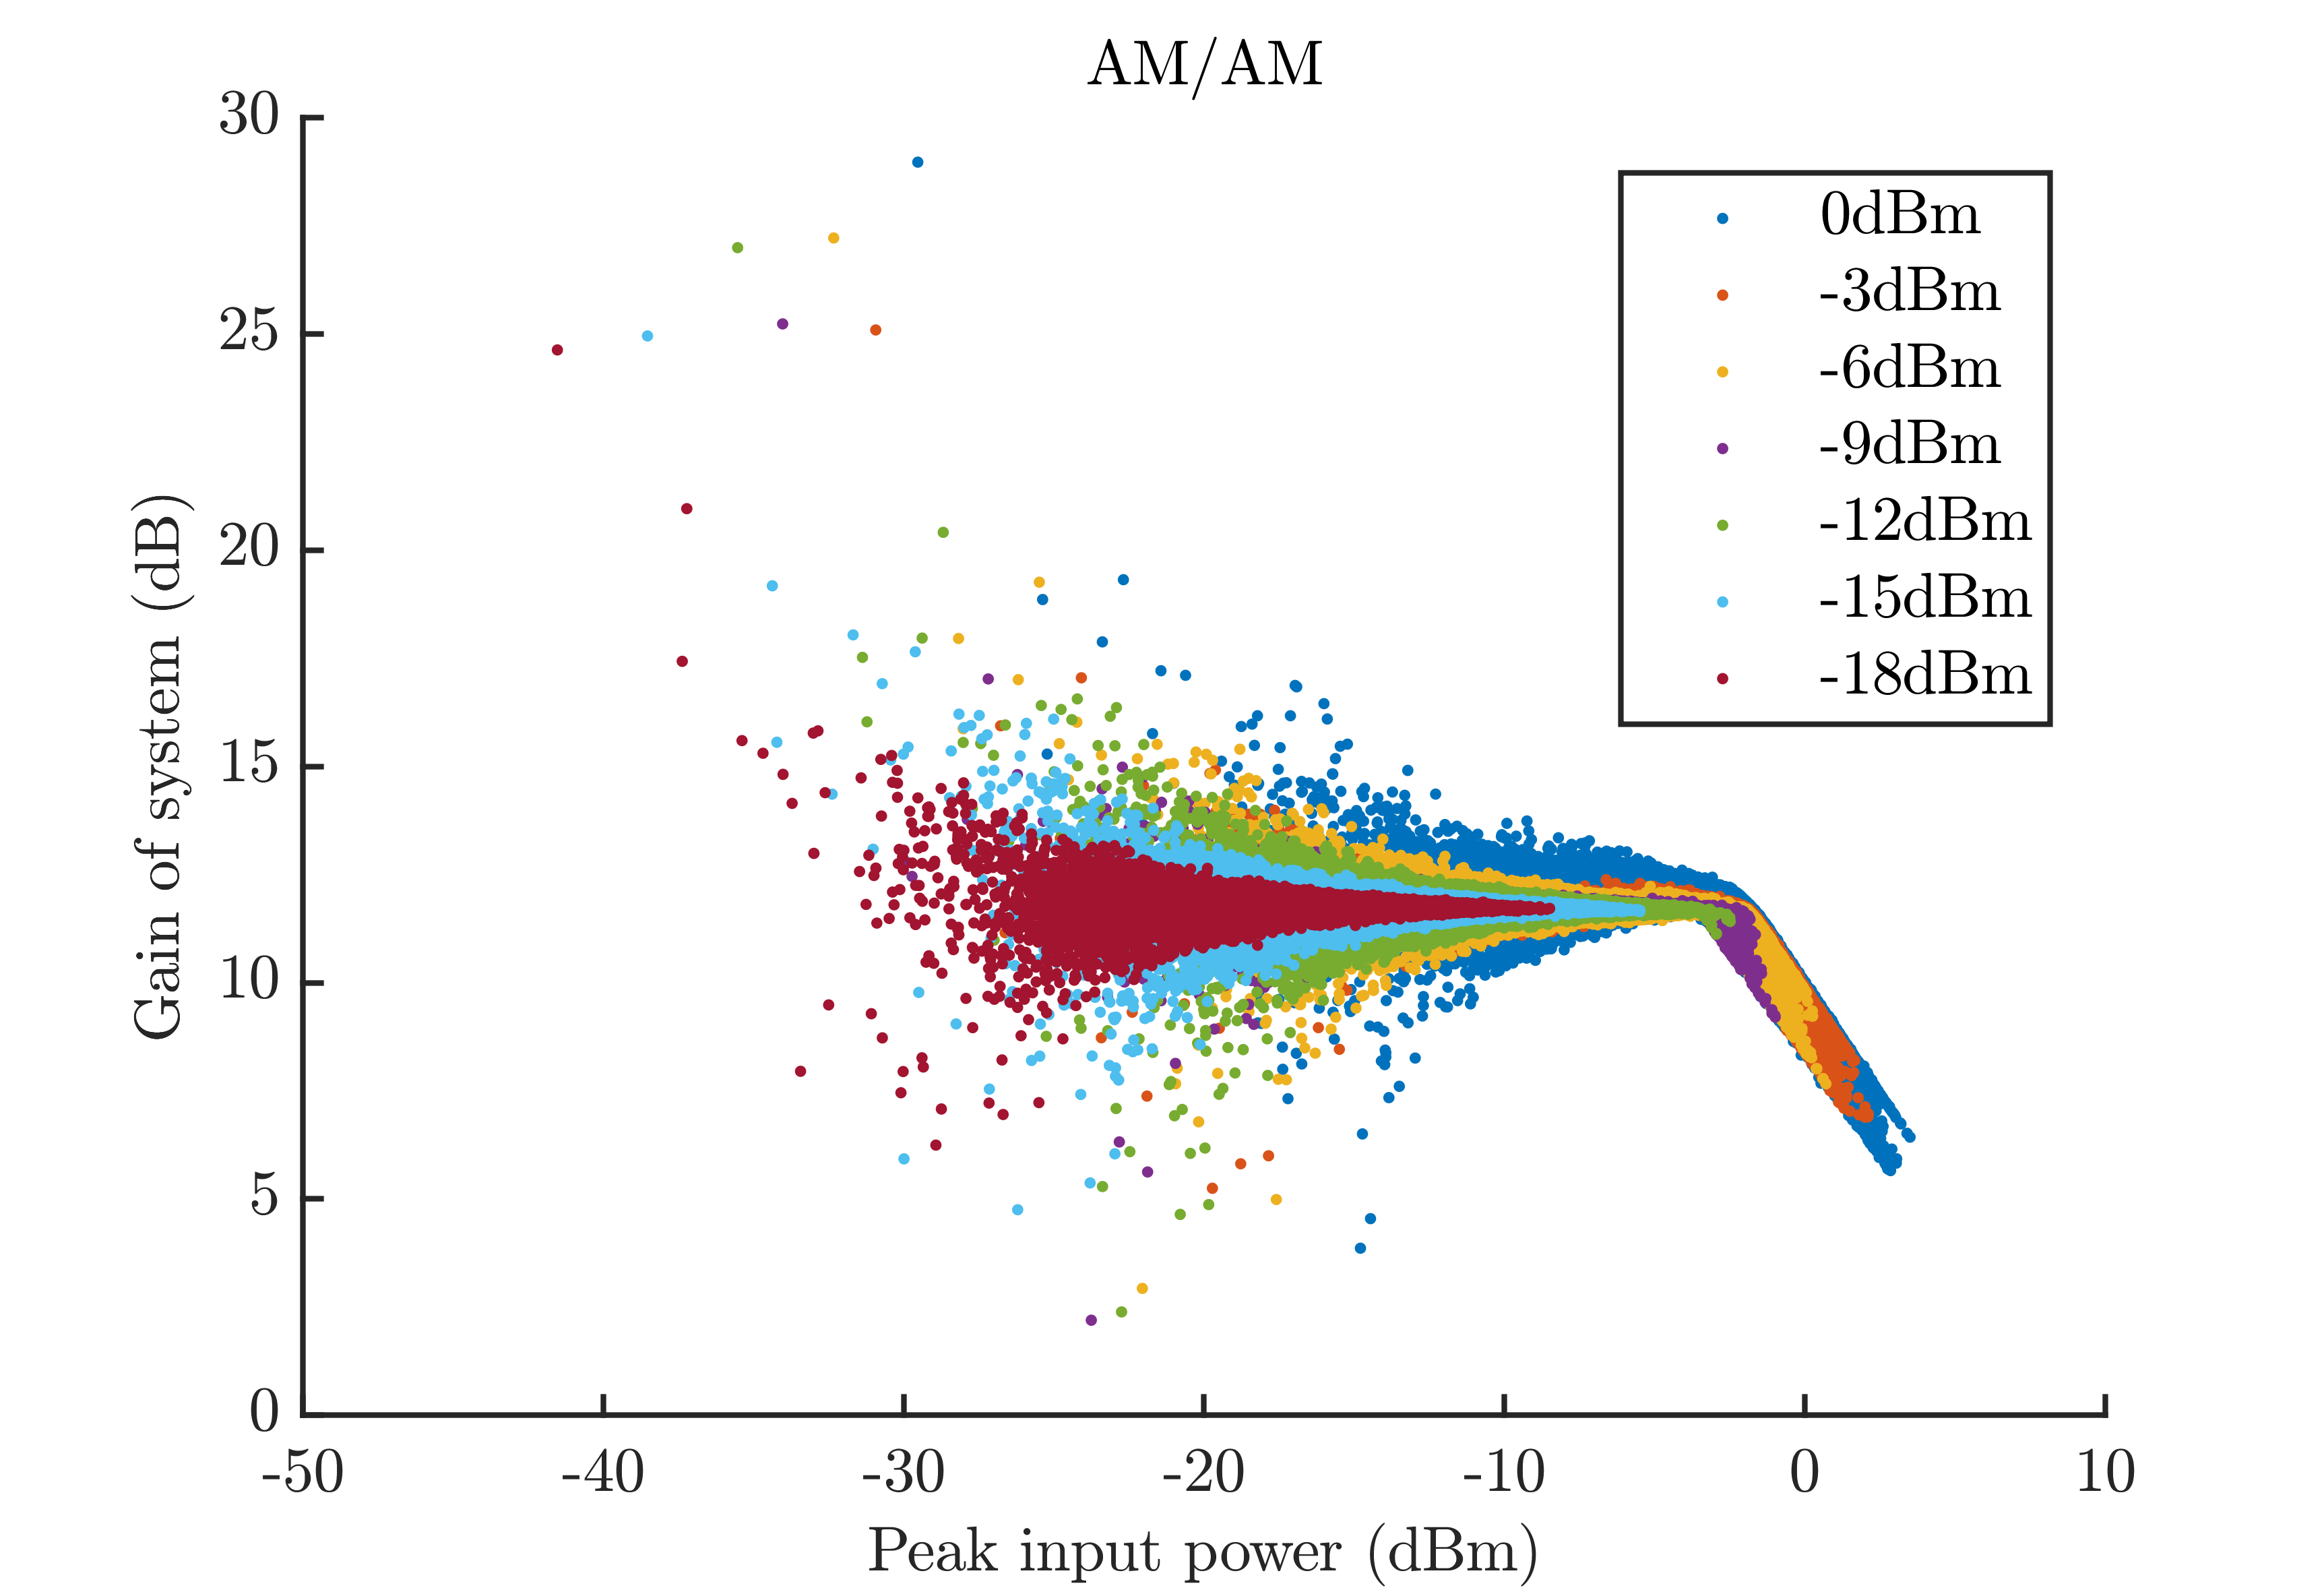
\includegraphics[scale = 0.5]{figures/measurement/four_antenna/amam_0p6.png}
\caption{AM/AM distortion at 0.6 $\lambda$ spacing between four antennas}
    \label{fig:amam06_4}
  \end{minipage}
\end{figure}


%%%%%%%%%%%%%%%%%%%%%%%%%%%%%%%%%%%%%%%%%%%%%%%%%%%%%%%%%%%%%%%%%%%%%%%%%%%%%%%%%%%%%%%%%%%%%%%%%%%%%%%%%%%%%%%%5
\subsection{PSD}
The Power Sprectal Density (PSD) shown in figure \ref{fig:psd_amp} is measured directly at the amplifier. It shows that at a mean input-power at 0dBm the output of the amplifier is distorted, first at a input level at -9dBm the distortion becomes low. This is also expected since the input is mean power and therefore the peak of the signal would be closely to -3dBm (6dB backoff) which also is close to the compression point measured in section \ref{ch:meas_amam}. Be aware that the noise floor increases due to the normalization of the signal. Also the reference-level at the spectrum analyser has an impact. When introducing the antenna system with one Tx antenna the distortion at -9dBm increases slightly. When introducing two antennas the distortion increases which is not a surprise due to the results from section \ref{ch:meas_amam}.  


\begin{figure}[H]
  \centering
  \begin{minipage}[b]{0.5\textwidth}
	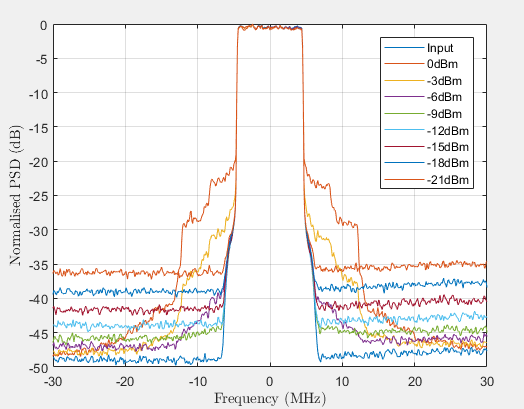
\includegraphics[scale = 0.5]{figures/measurement/two_antenna/amplifier_psd.png}
	\caption{PSD at amplifier}
    \label{fig:psd_amp}
  \end{minipage}
  \hfill
  \begin{minipage}[b]{0.4\textwidth}
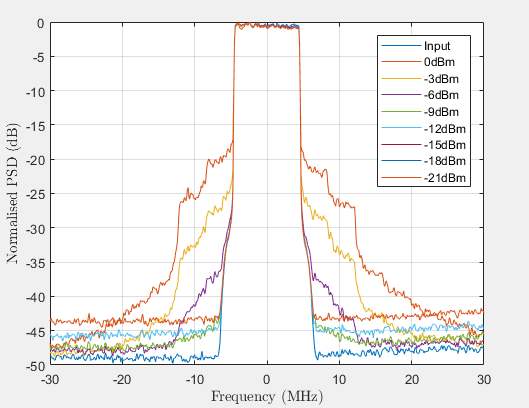
\includegraphics[scale = 0.5]{figures/measurement/two_antenna/one_ant_psd.png}
\caption{PSD using one transmit antenna}
    \label{fig:psd_one_ant}
  \end{minipage}
\end{figure}

\subsubsection{Two transmit antenna}

\begin{figure}[H]
  \centering
  \begin{minipage}[b]{0.5\textwidth}
	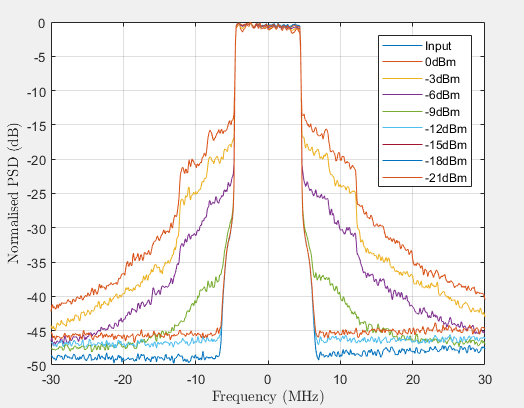
\includegraphics[scale = 0.5]{figures/measurement/two_antenna/psd_01.png}
	\caption{PSD at 0.1 $\lambda$ spacing between two antennas}
    \label{fig:psd01}
  \end{minipage}
  \hfill
  \begin{minipage}[b]{0.4\textwidth}
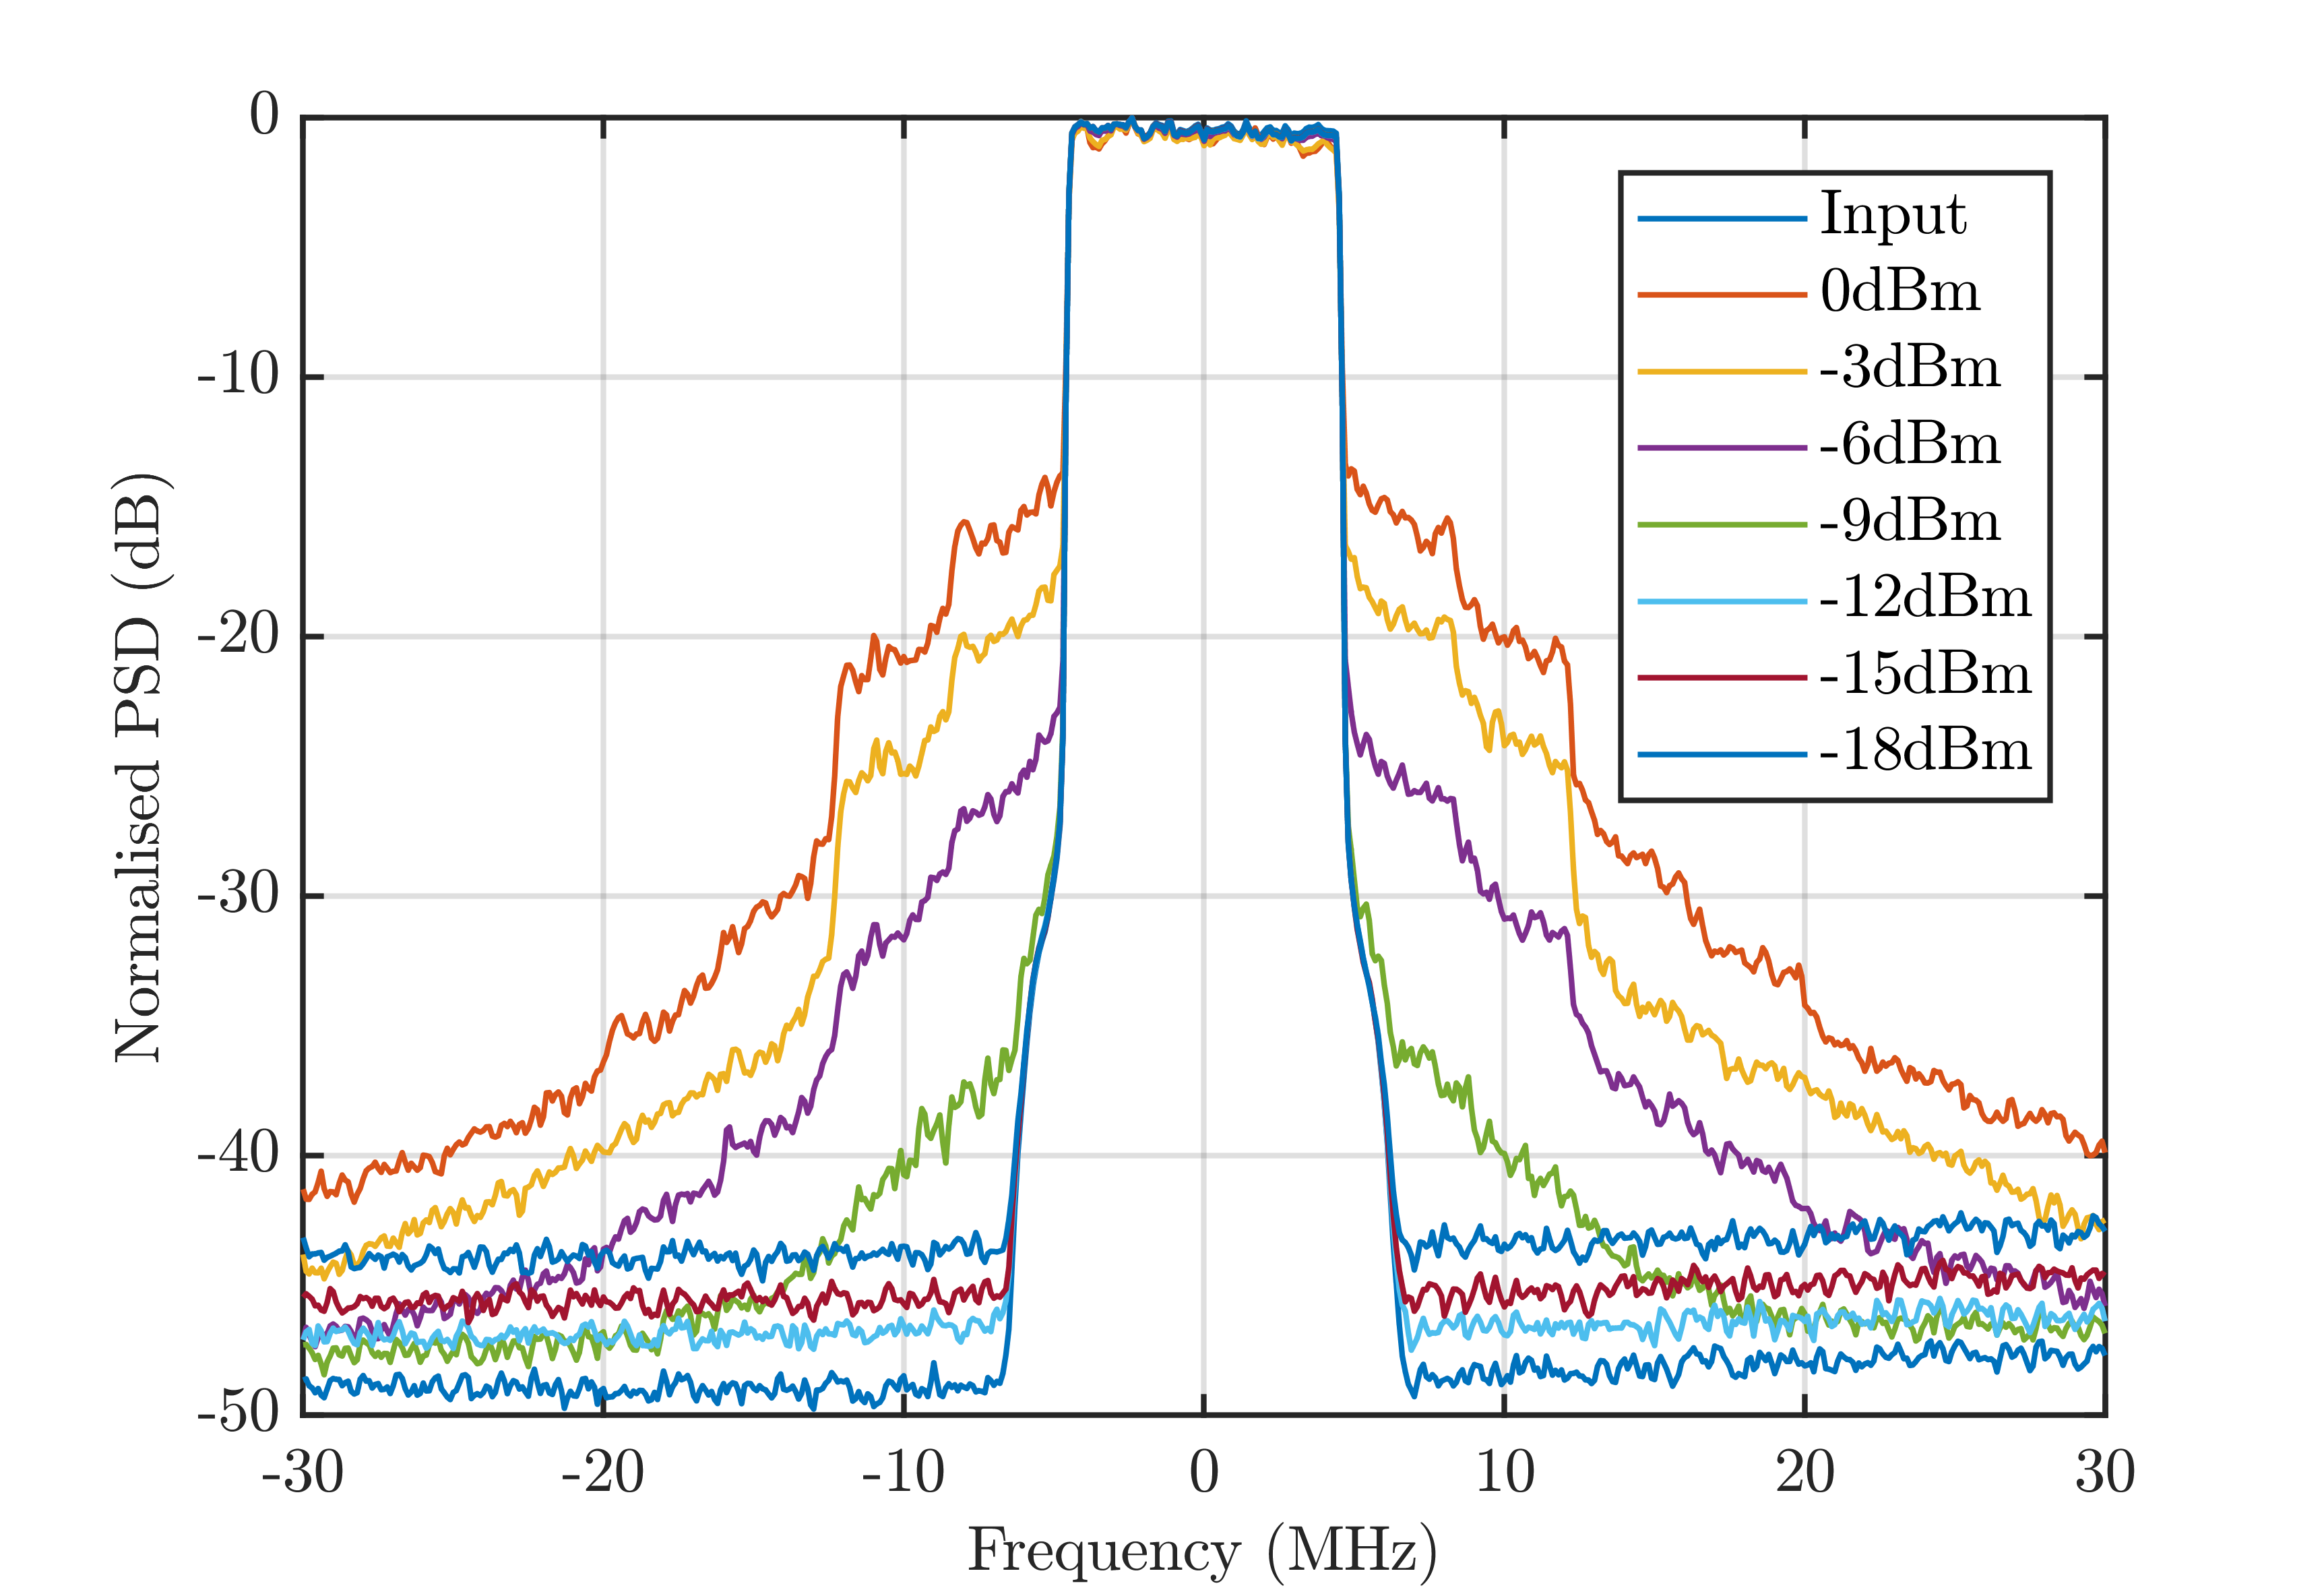
\includegraphics[scale = 0.5]{figures/measurement/two_antenna/psd_02.png}
\caption{PSD at 0.2 $\lambda$ spacing between two antennas}
    \label{fig:psd02}
  \end{minipage}
\end{figure}

\begin{figure}[H]
  \centering
  \begin{minipage}[b]{0.5\textwidth}
	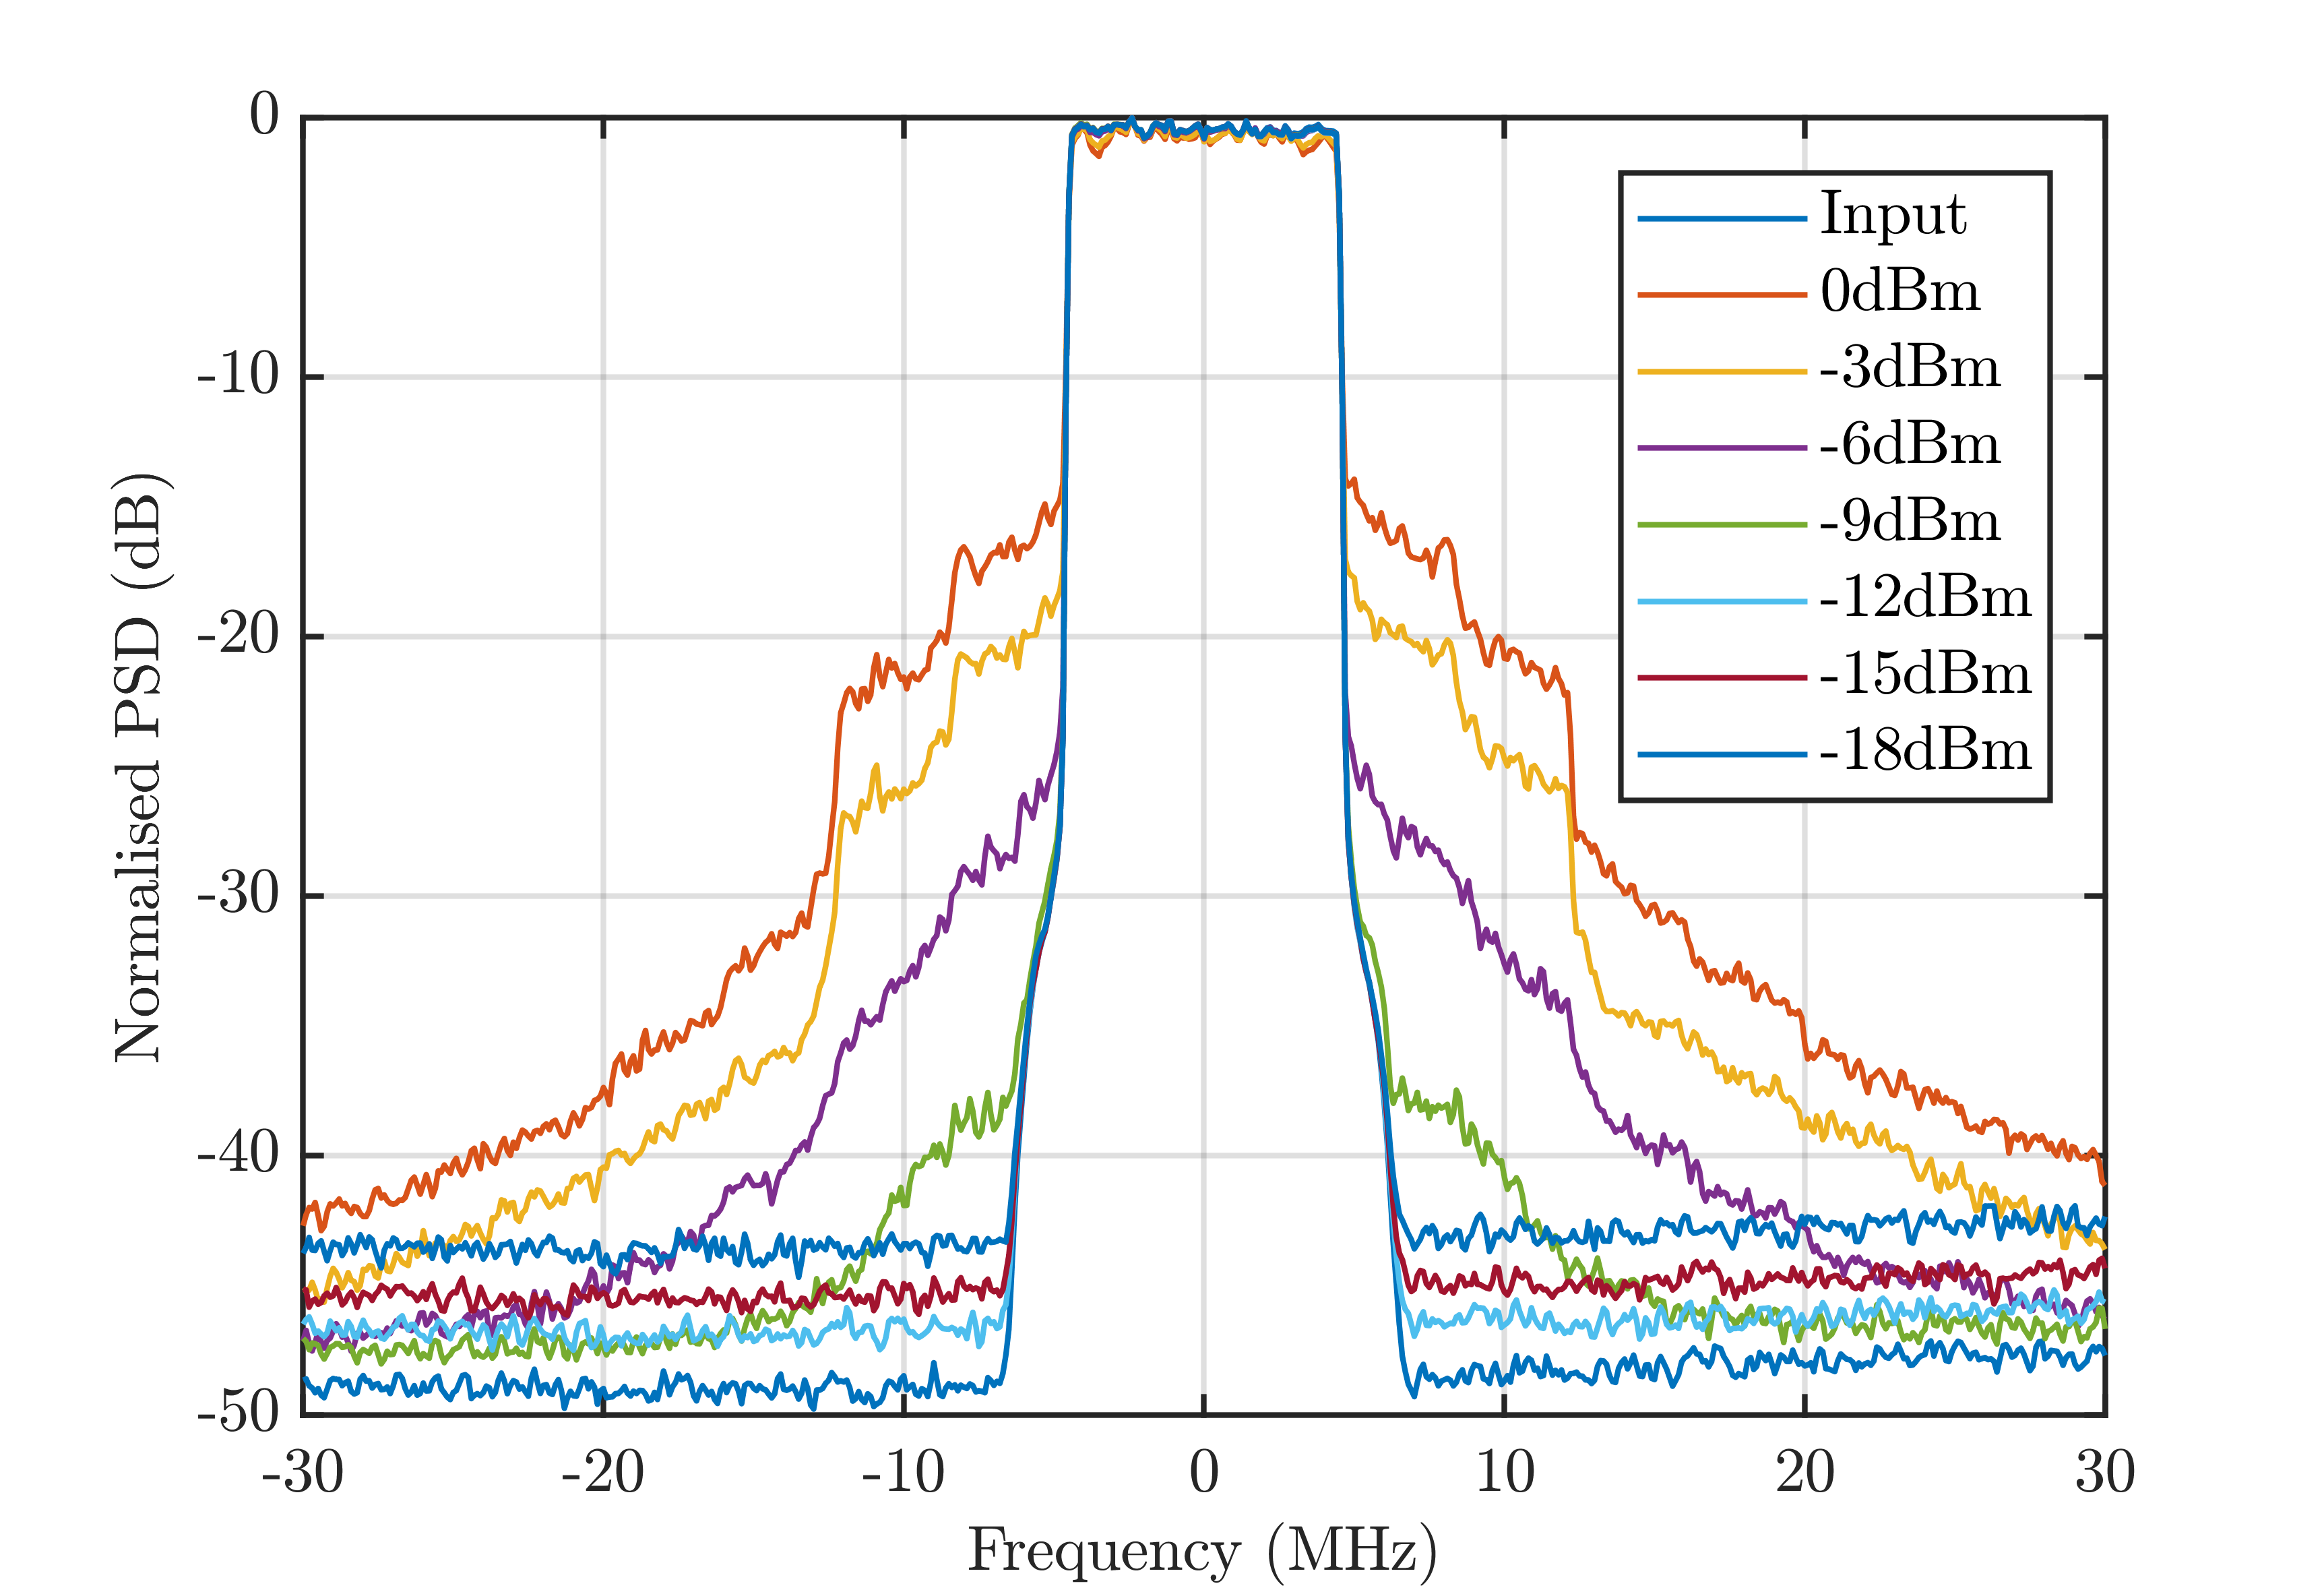
\includegraphics[scale = 0.5]{figures/measurement/two_antenna/psd_03.png}
	\caption{PSD at 0.3 $\lambda$ spacing between two antennas}
    \label{fig:psd03}
  \end{minipage}
  \hfill
  \begin{minipage}[b]{0.4\textwidth}
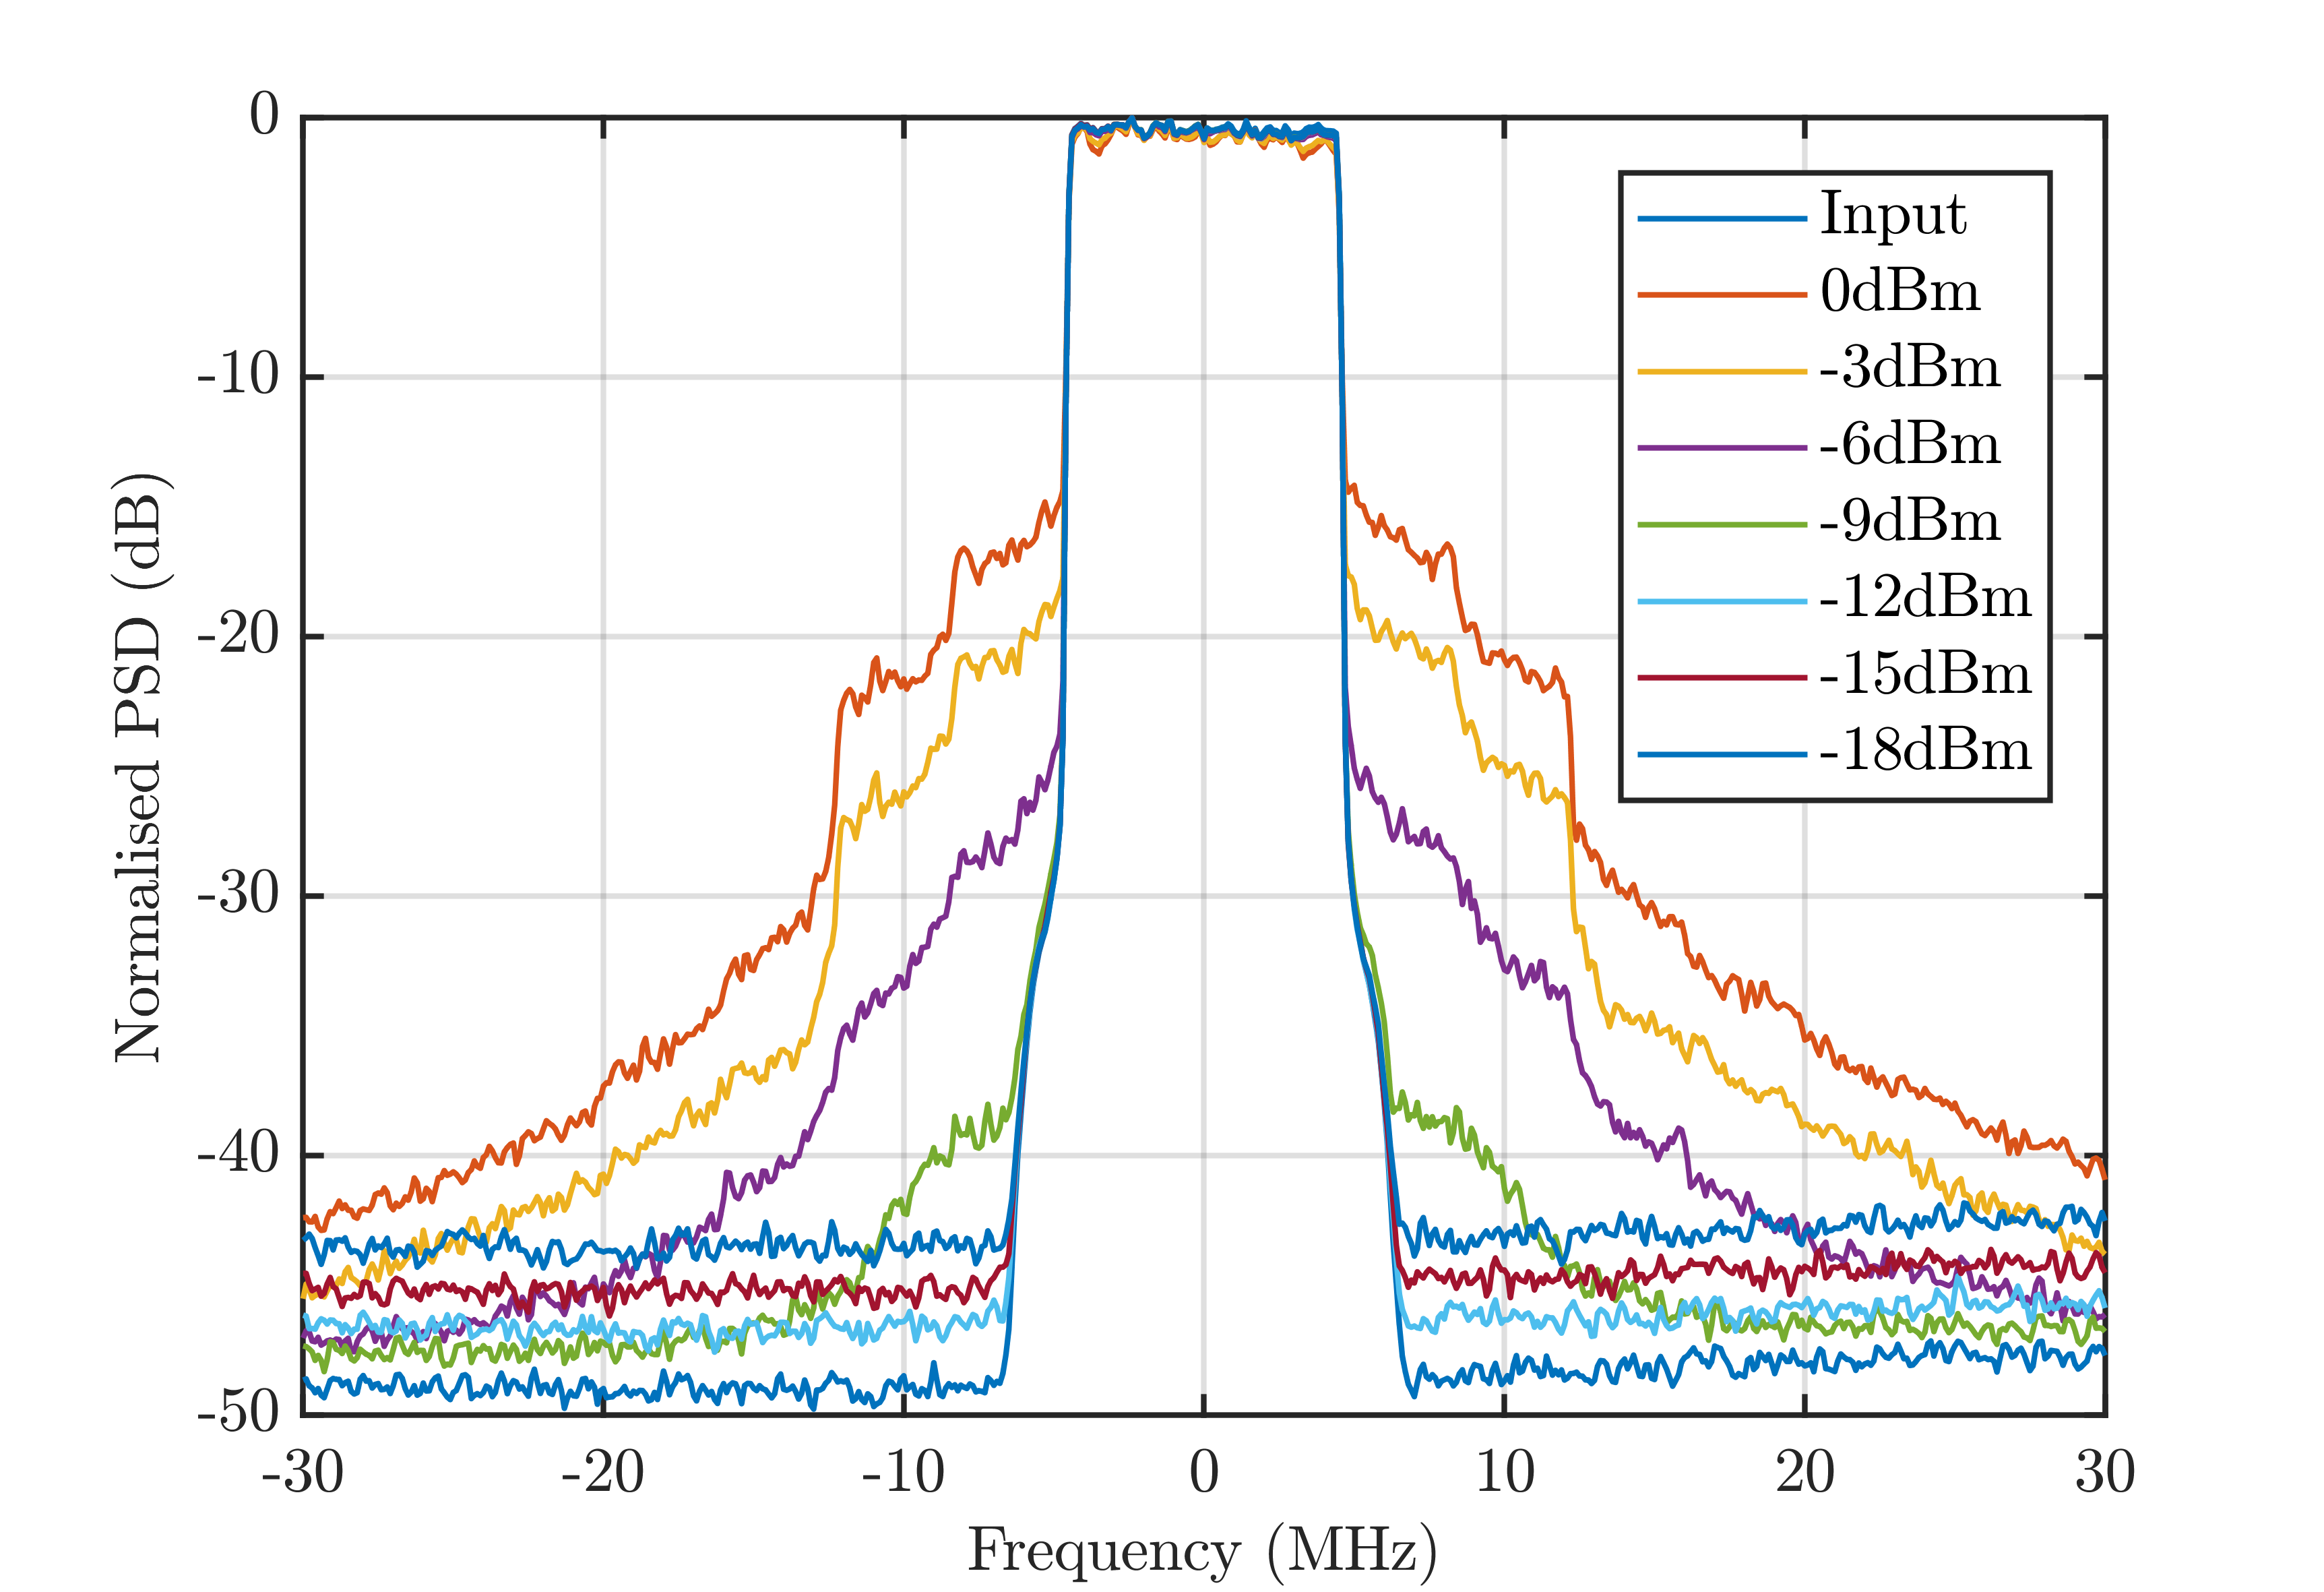
\includegraphics[scale = 0.5]{figures/measurement/two_antenna/psd_04.png}
\caption{PSD at 0.4 $\lambda$ spacing between two antennas}
    \label{fig:psd04}
  \end{minipage}
\end{figure}

\begin{figure}[H]
  \centering
  \begin{minipage}[b]{0.5\textwidth}
	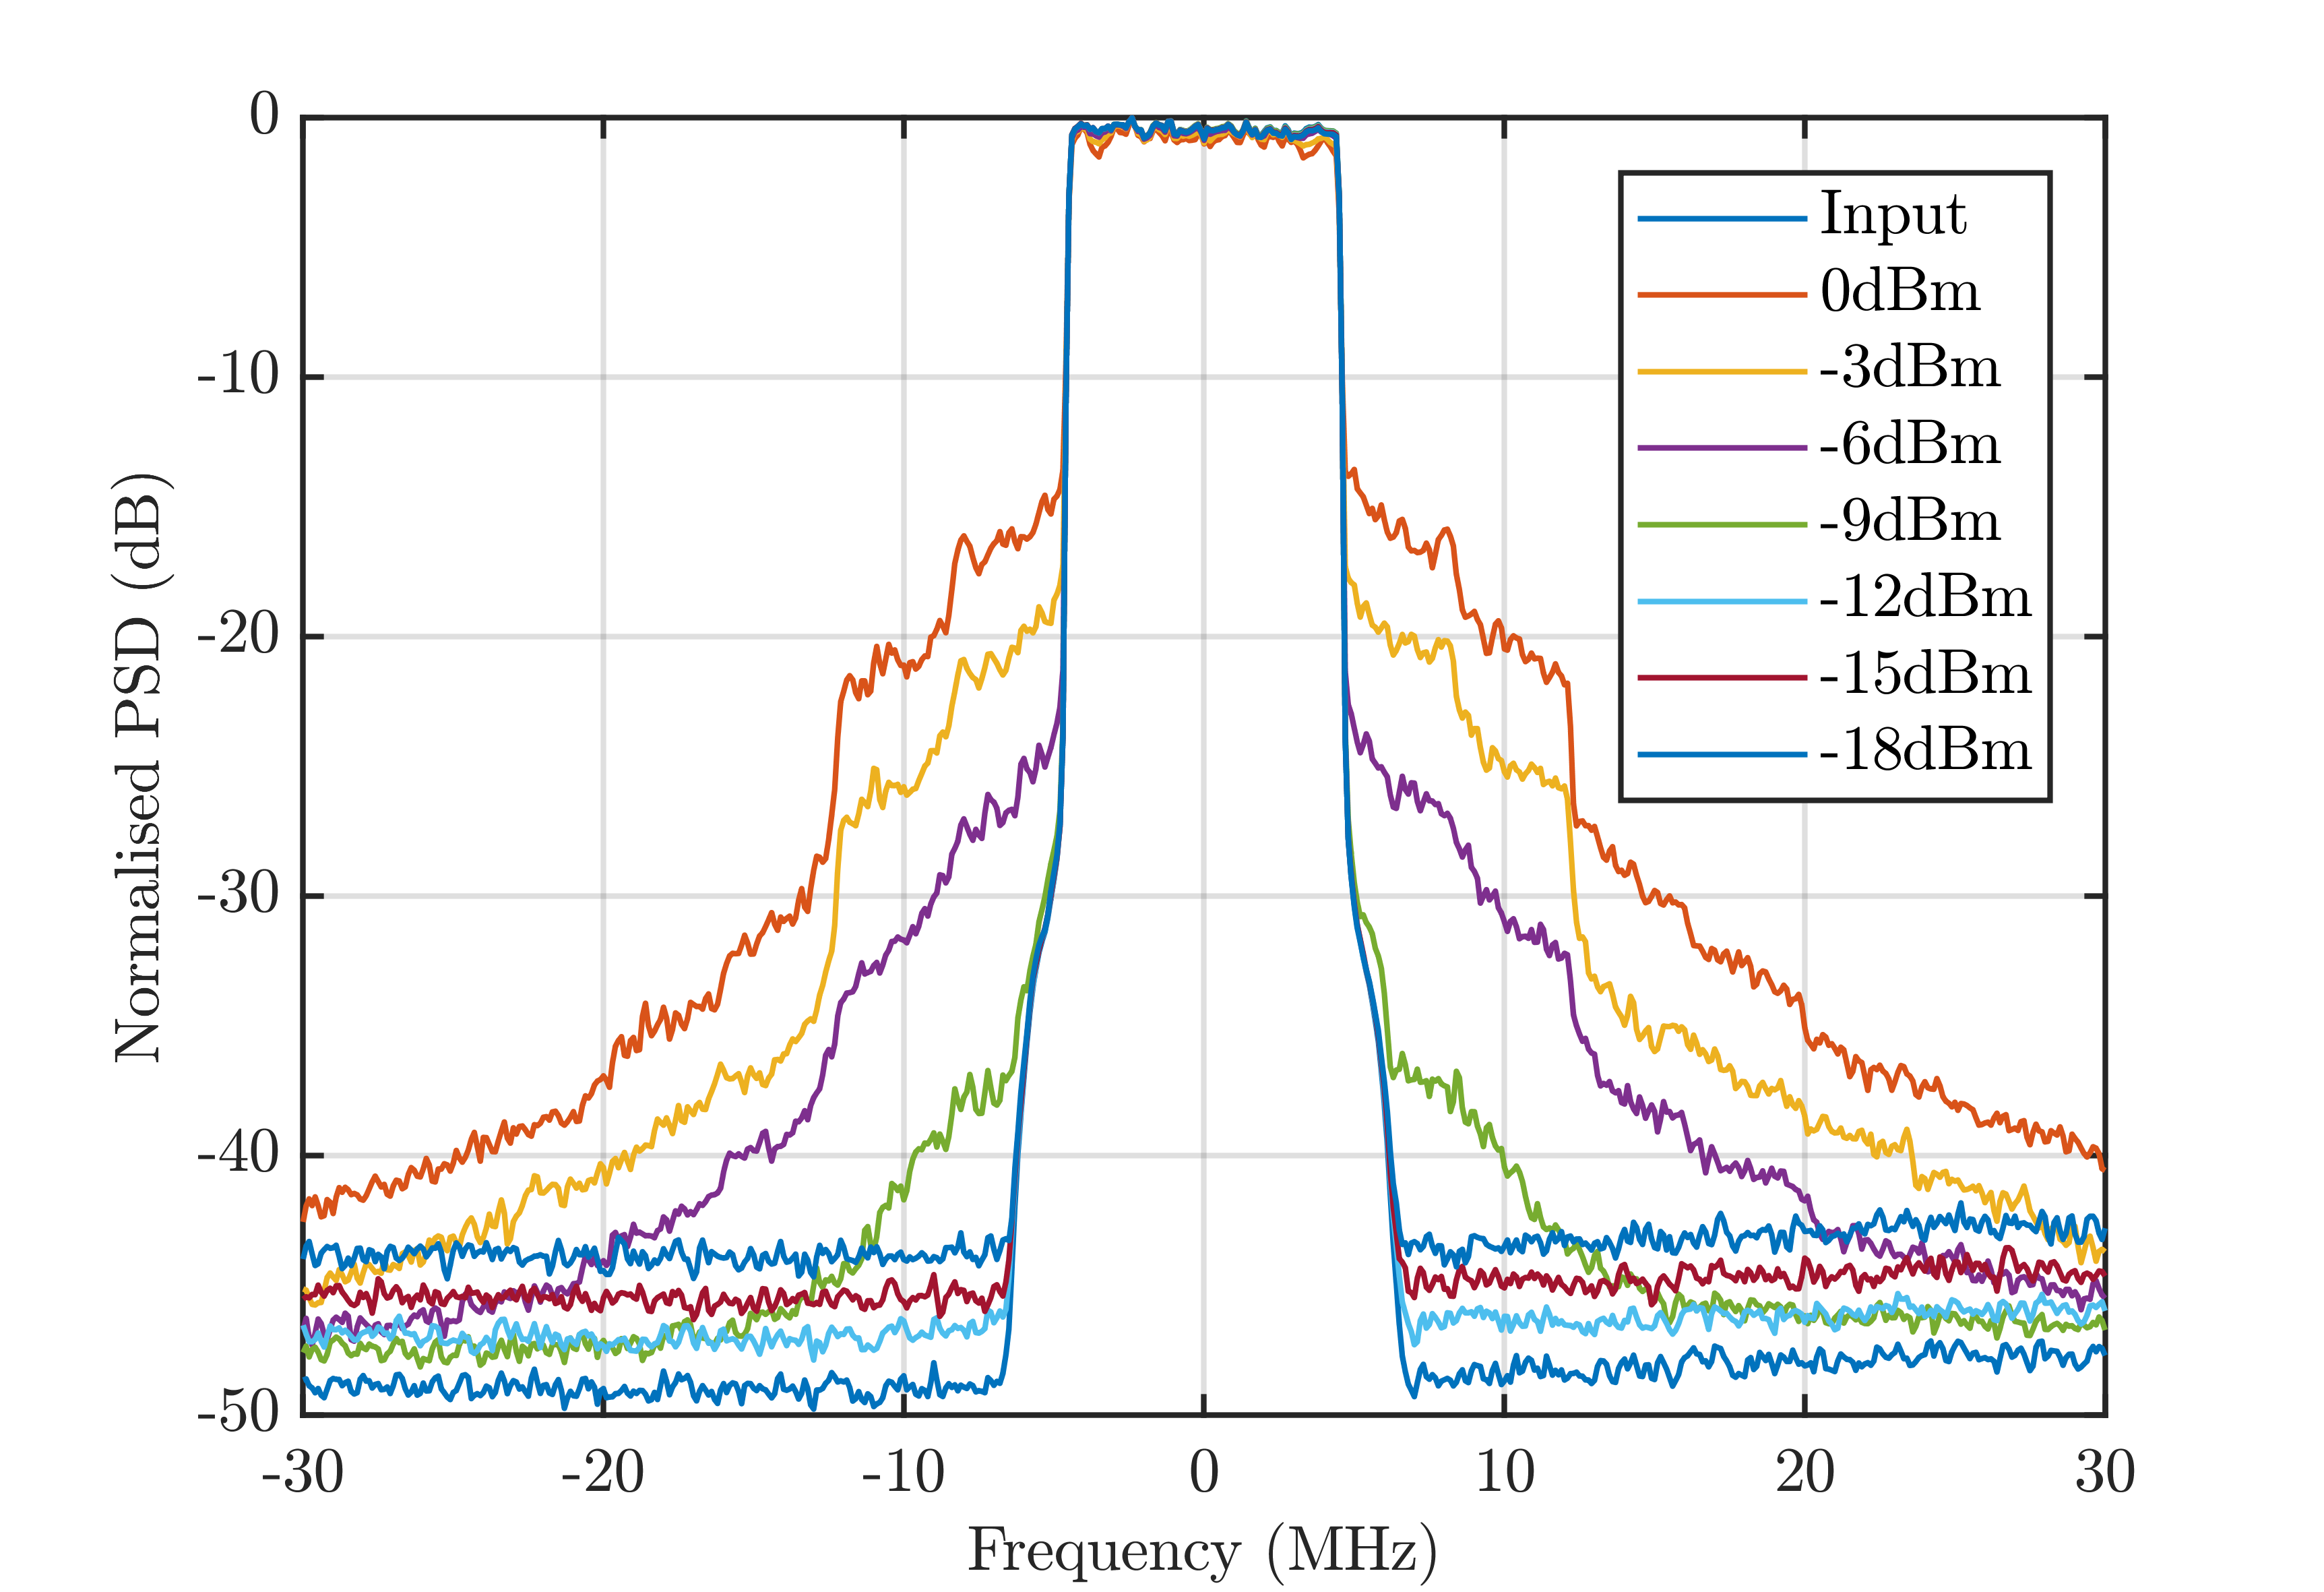
\includegraphics[scale = 0.5]{figures/measurement/two_antenna/psd_05.png}
	\caption{PSD at 0.5 $\lambda$ spacing between two antennas}
    \label{fig:psd05}
  \end{minipage}
  \hfill
  \begin{minipage}[b]{0.4\textwidth}
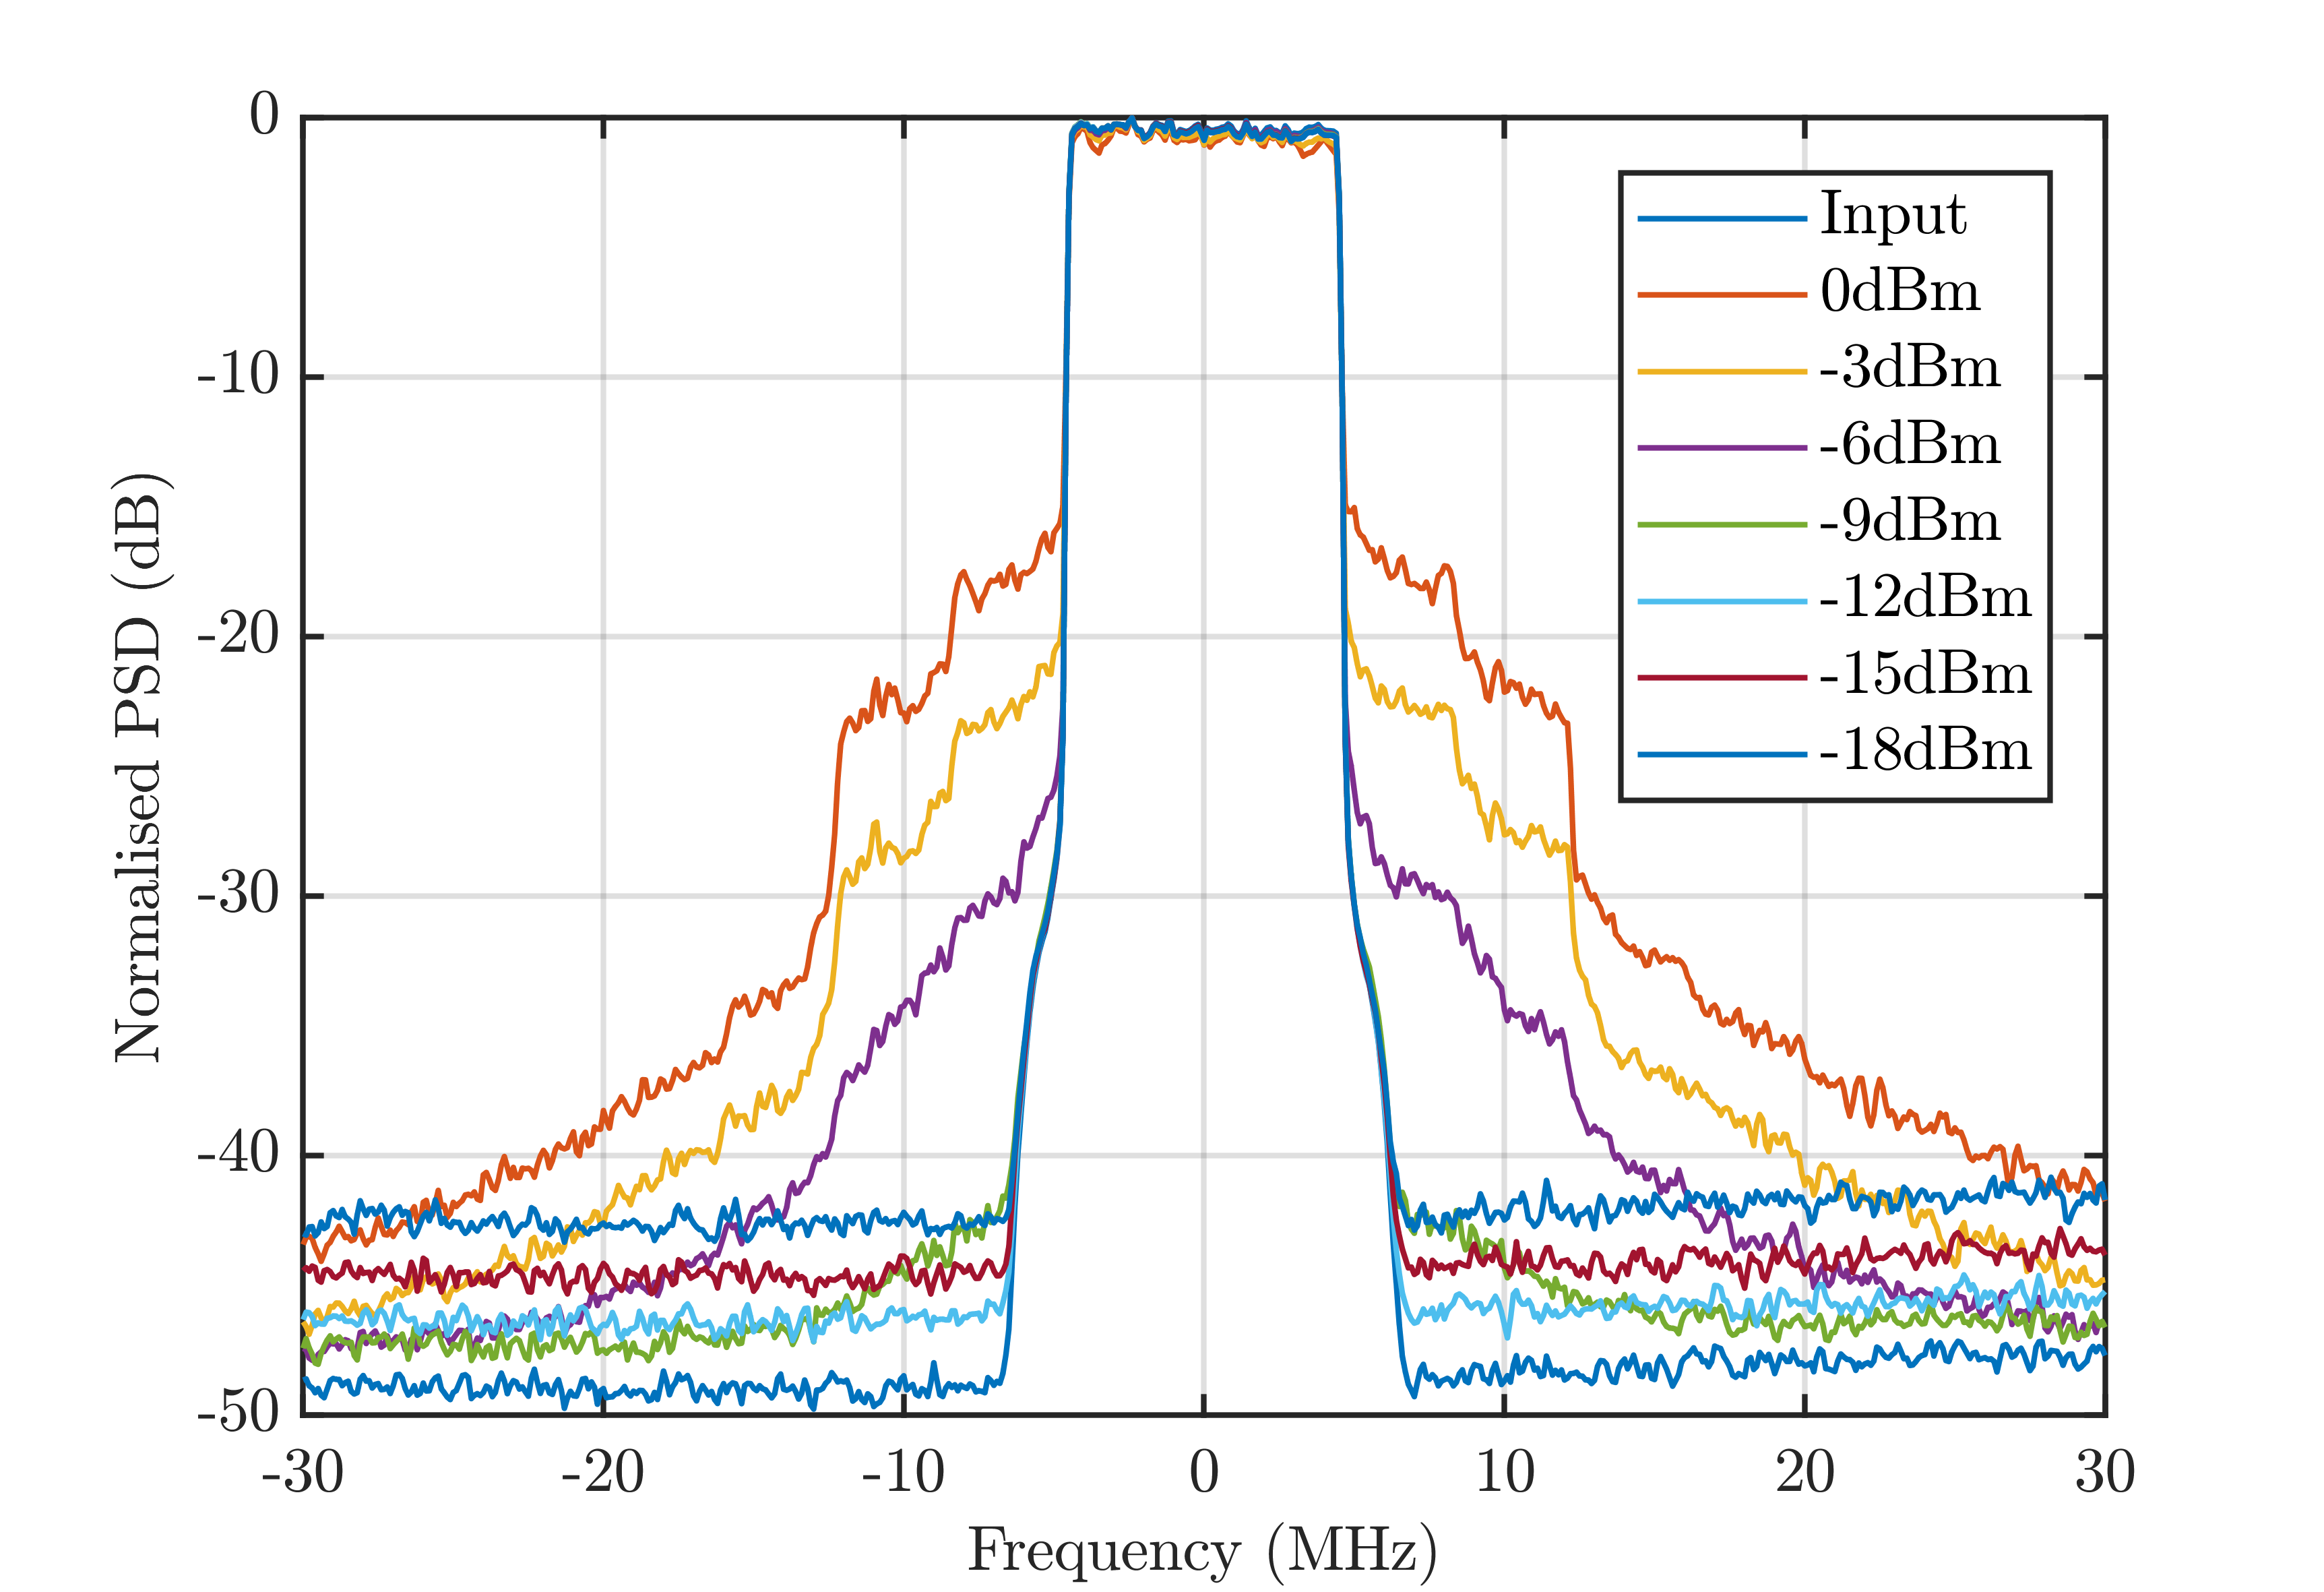
\includegraphics[scale = 0.5]{figures/measurement/two_antenna/psd_06.png}
\caption{PSD at 0.6 $\lambda$ spacing between two antennas}
    \label{fig:psd06}
  \end{minipage}
\end{figure}

\subsubsection{Four transmit antenna}

\begin{figure}[H]
  \centering
  \begin{minipage}[b]{0.5\textwidth}
	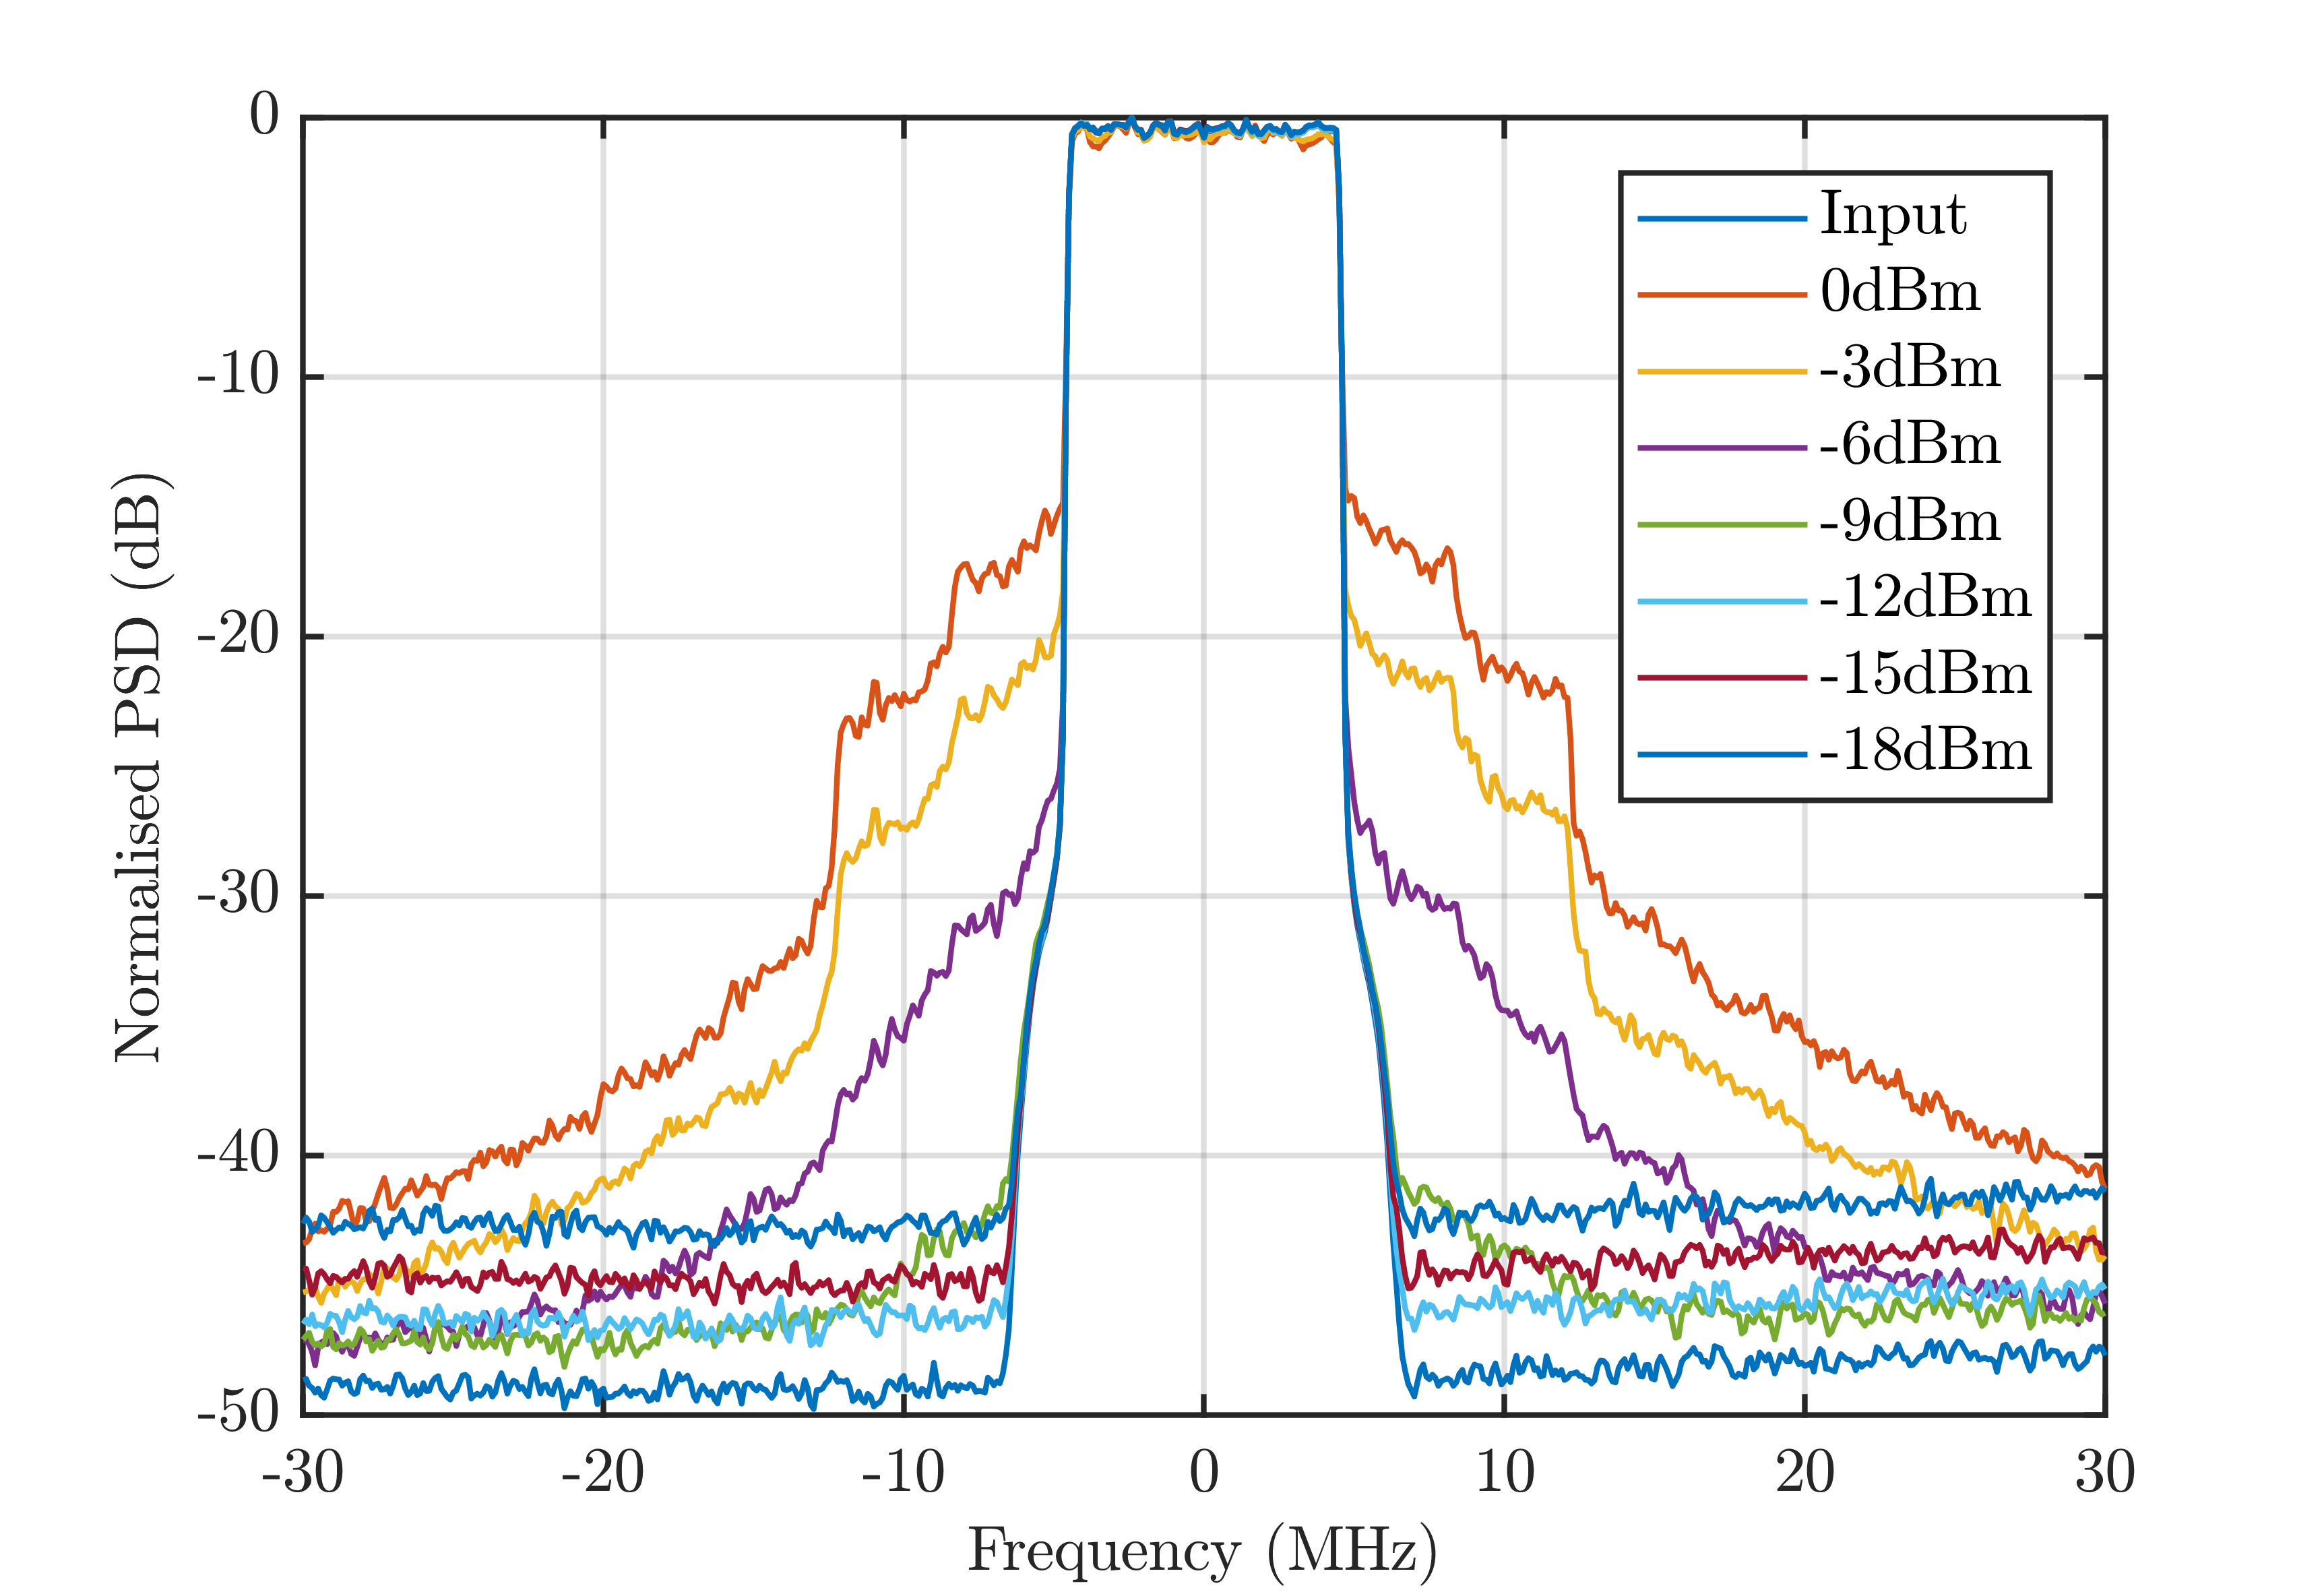
\includegraphics[scale = 0.5]{figures/measurement/four_antenna/psd_0p1.png}
	\caption{PSD at 0.1 $\lambda$ spacing between four antennas}
    \label{fig:psd01_4}
  \end{minipage}
  \hfill
  \begin{minipage}[b]{0.4\textwidth}
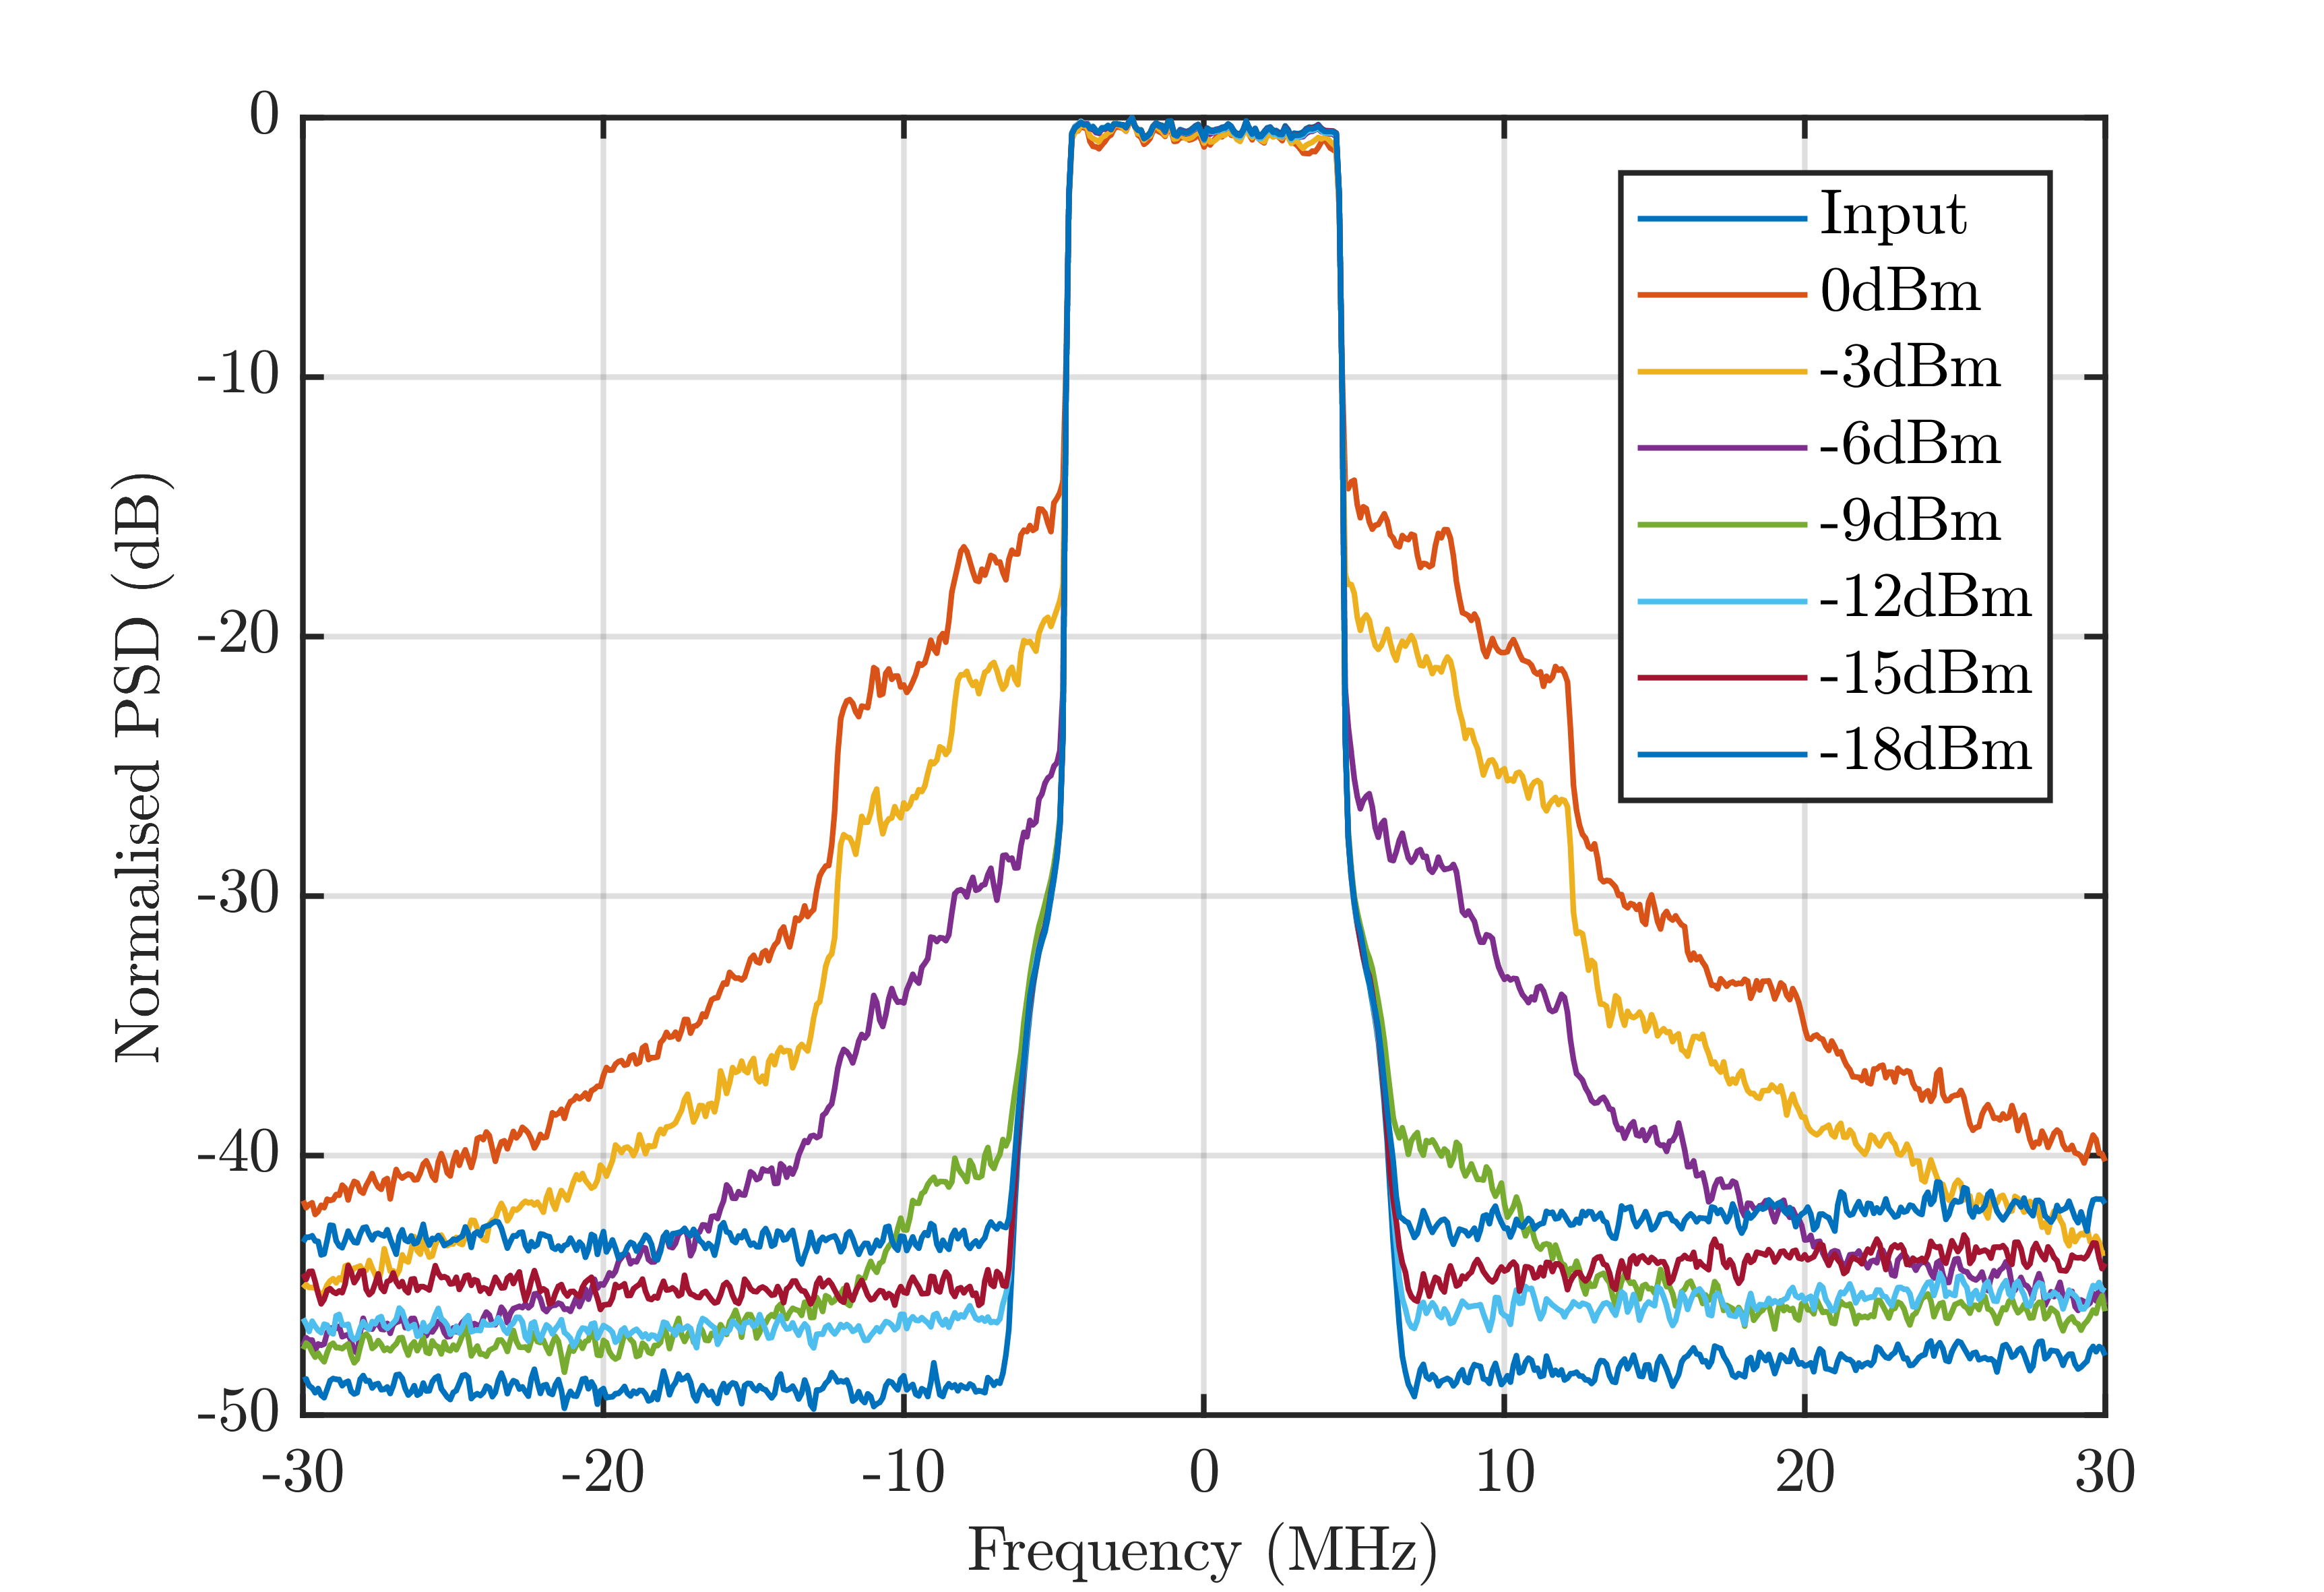
\includegraphics[scale = 0.5]{figures/measurement/four_antenna/psd_0p2.png}
\caption{PSD at 0.2 $\lambda$ spacing between four antennas}
    \label{fig:psd02_4}
  \end{minipage}
\end{figure}

\begin{figure}[H]
  \centering
  \begin{minipage}[b]{0.5\textwidth}
	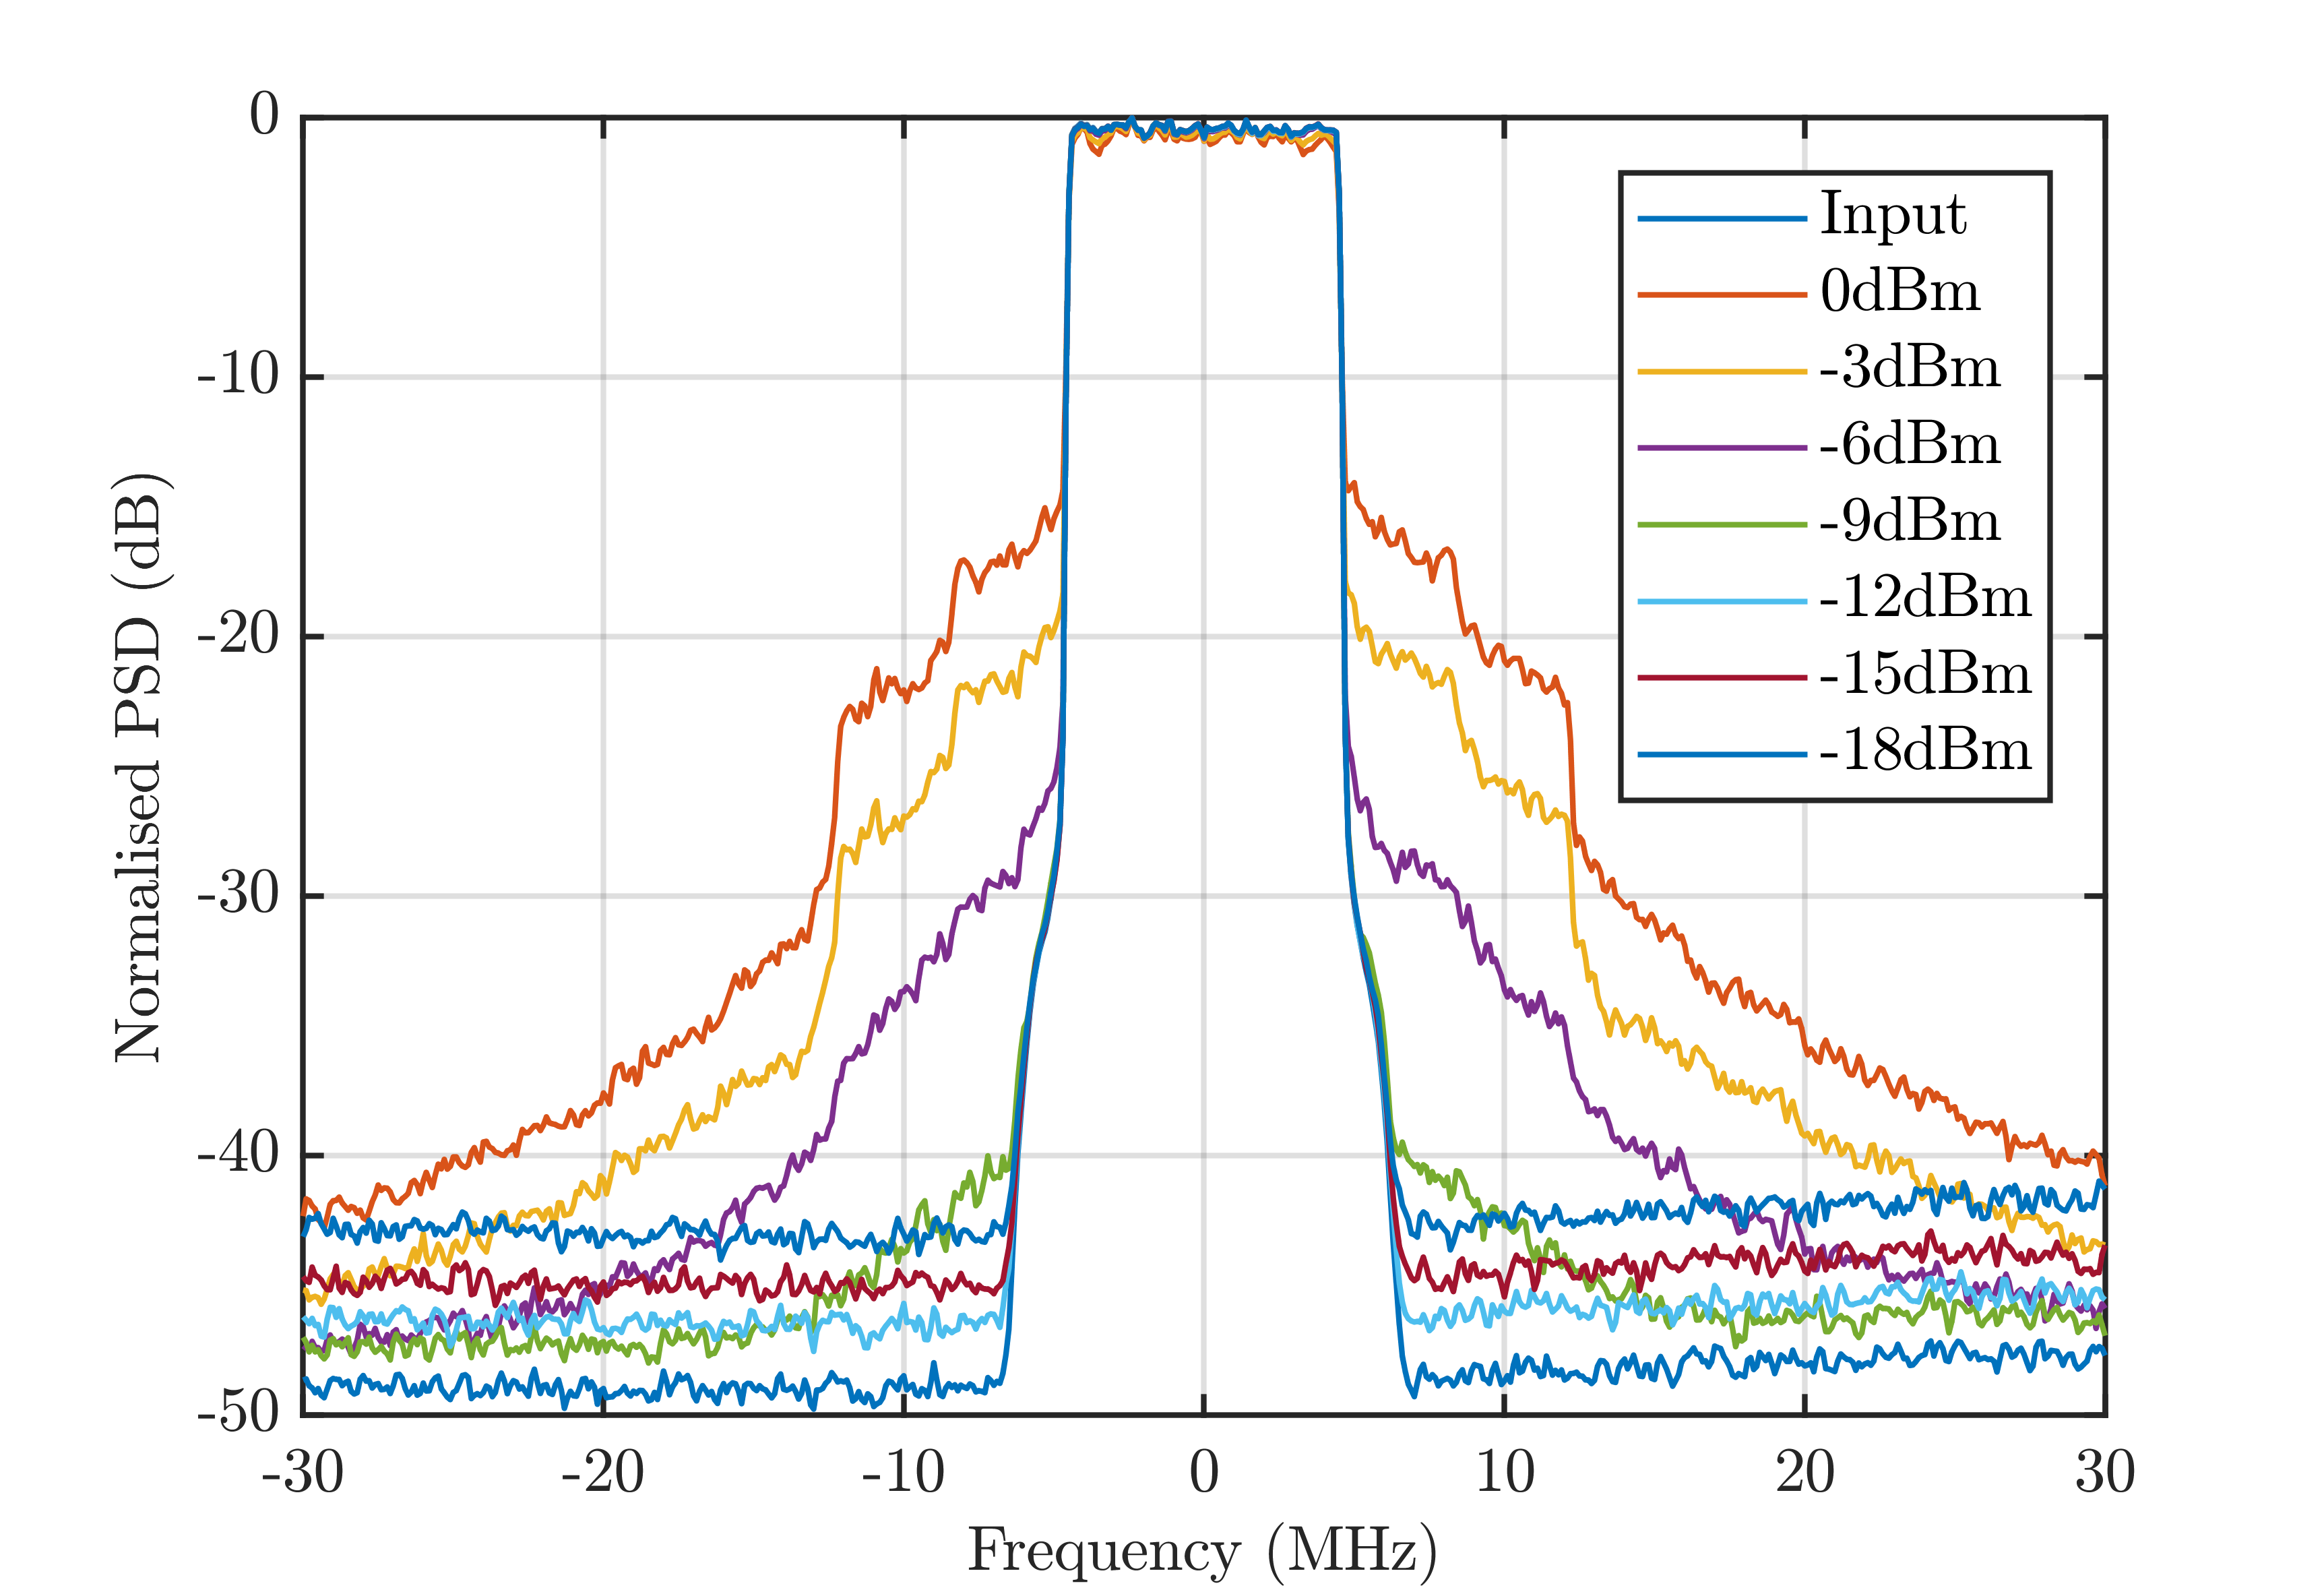
\includegraphics[scale = 0.5]{figures/measurement/four_antenna/psd_0p3.png}
	\caption{PSD at 0.3 $\lambda$ spacing between four antennas}
    \label{fig:psd03_4}
  \end{minipage}
  \hfill
  \begin{minipage}[b]{0.4\textwidth}
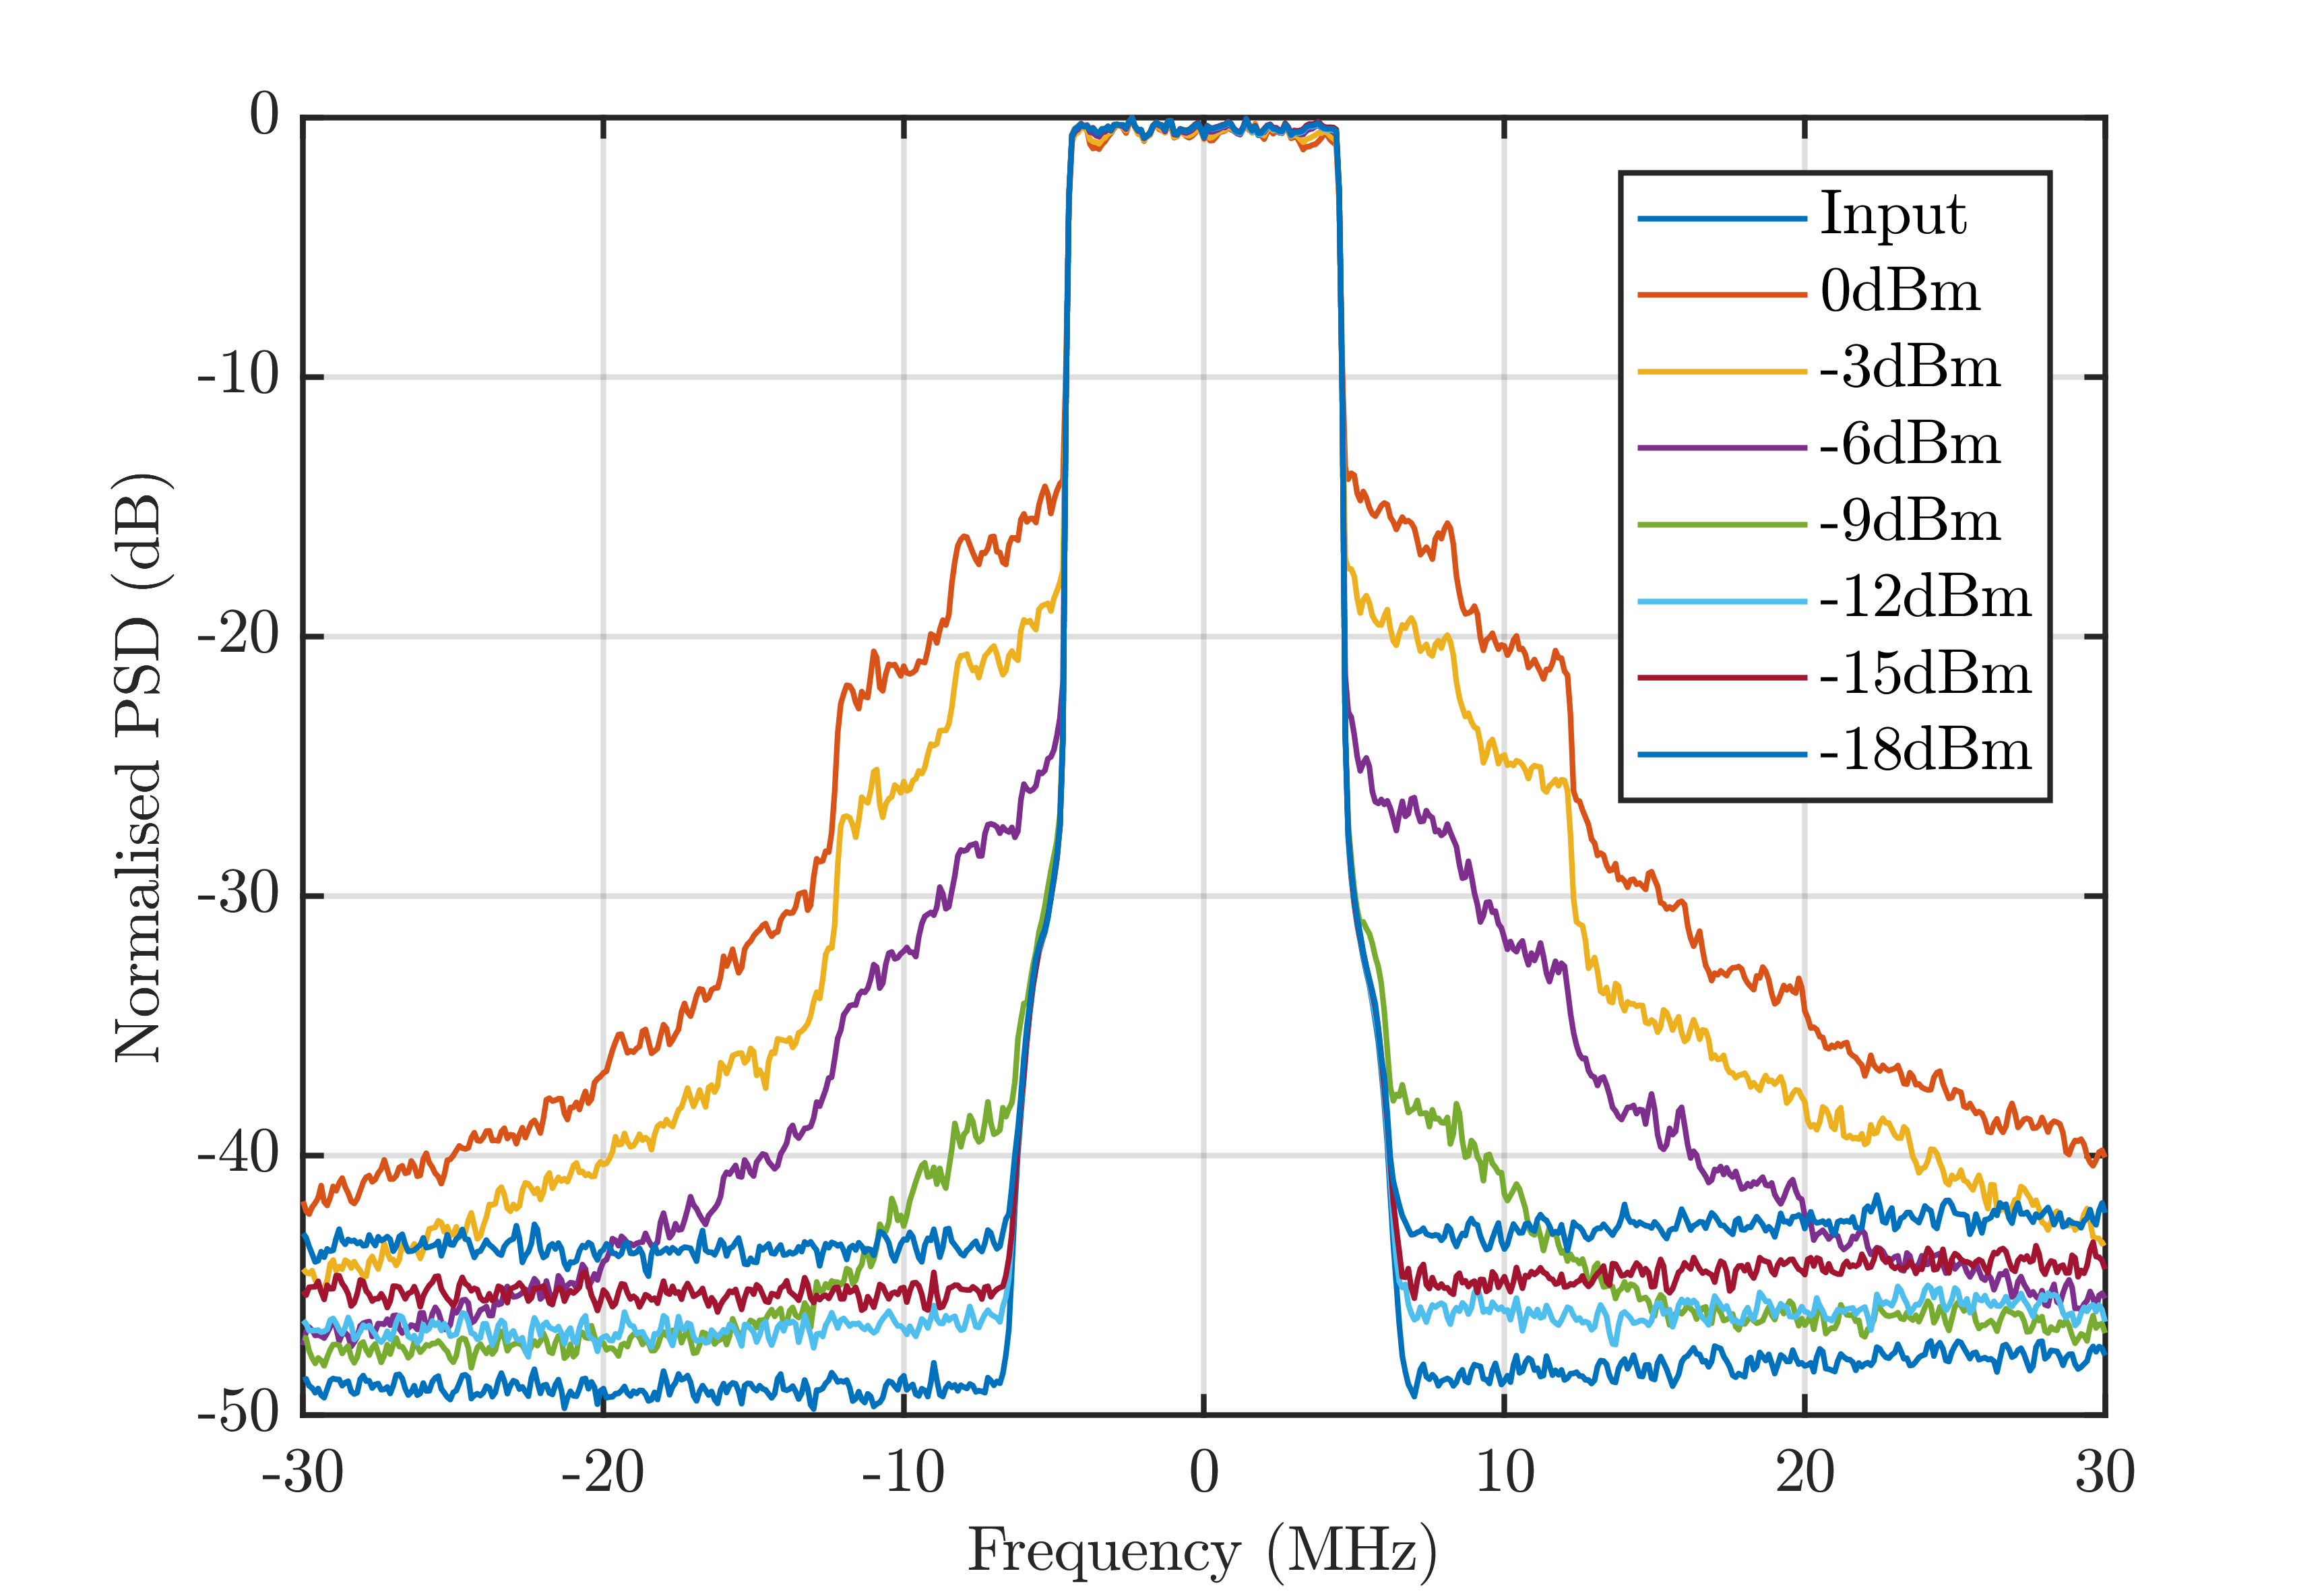
\includegraphics[scale = 0.5]{figures/measurement/four_antenna/psd_0p4.png}
\caption{PSD at 0.4 $\lambda$ spacing between four antennas}
    \label{fig:psd04_4}
  \end{minipage}
\end{figure}

\begin{figure}[H]
  \centering
  \begin{minipage}[b]{0.5\textwidth}
	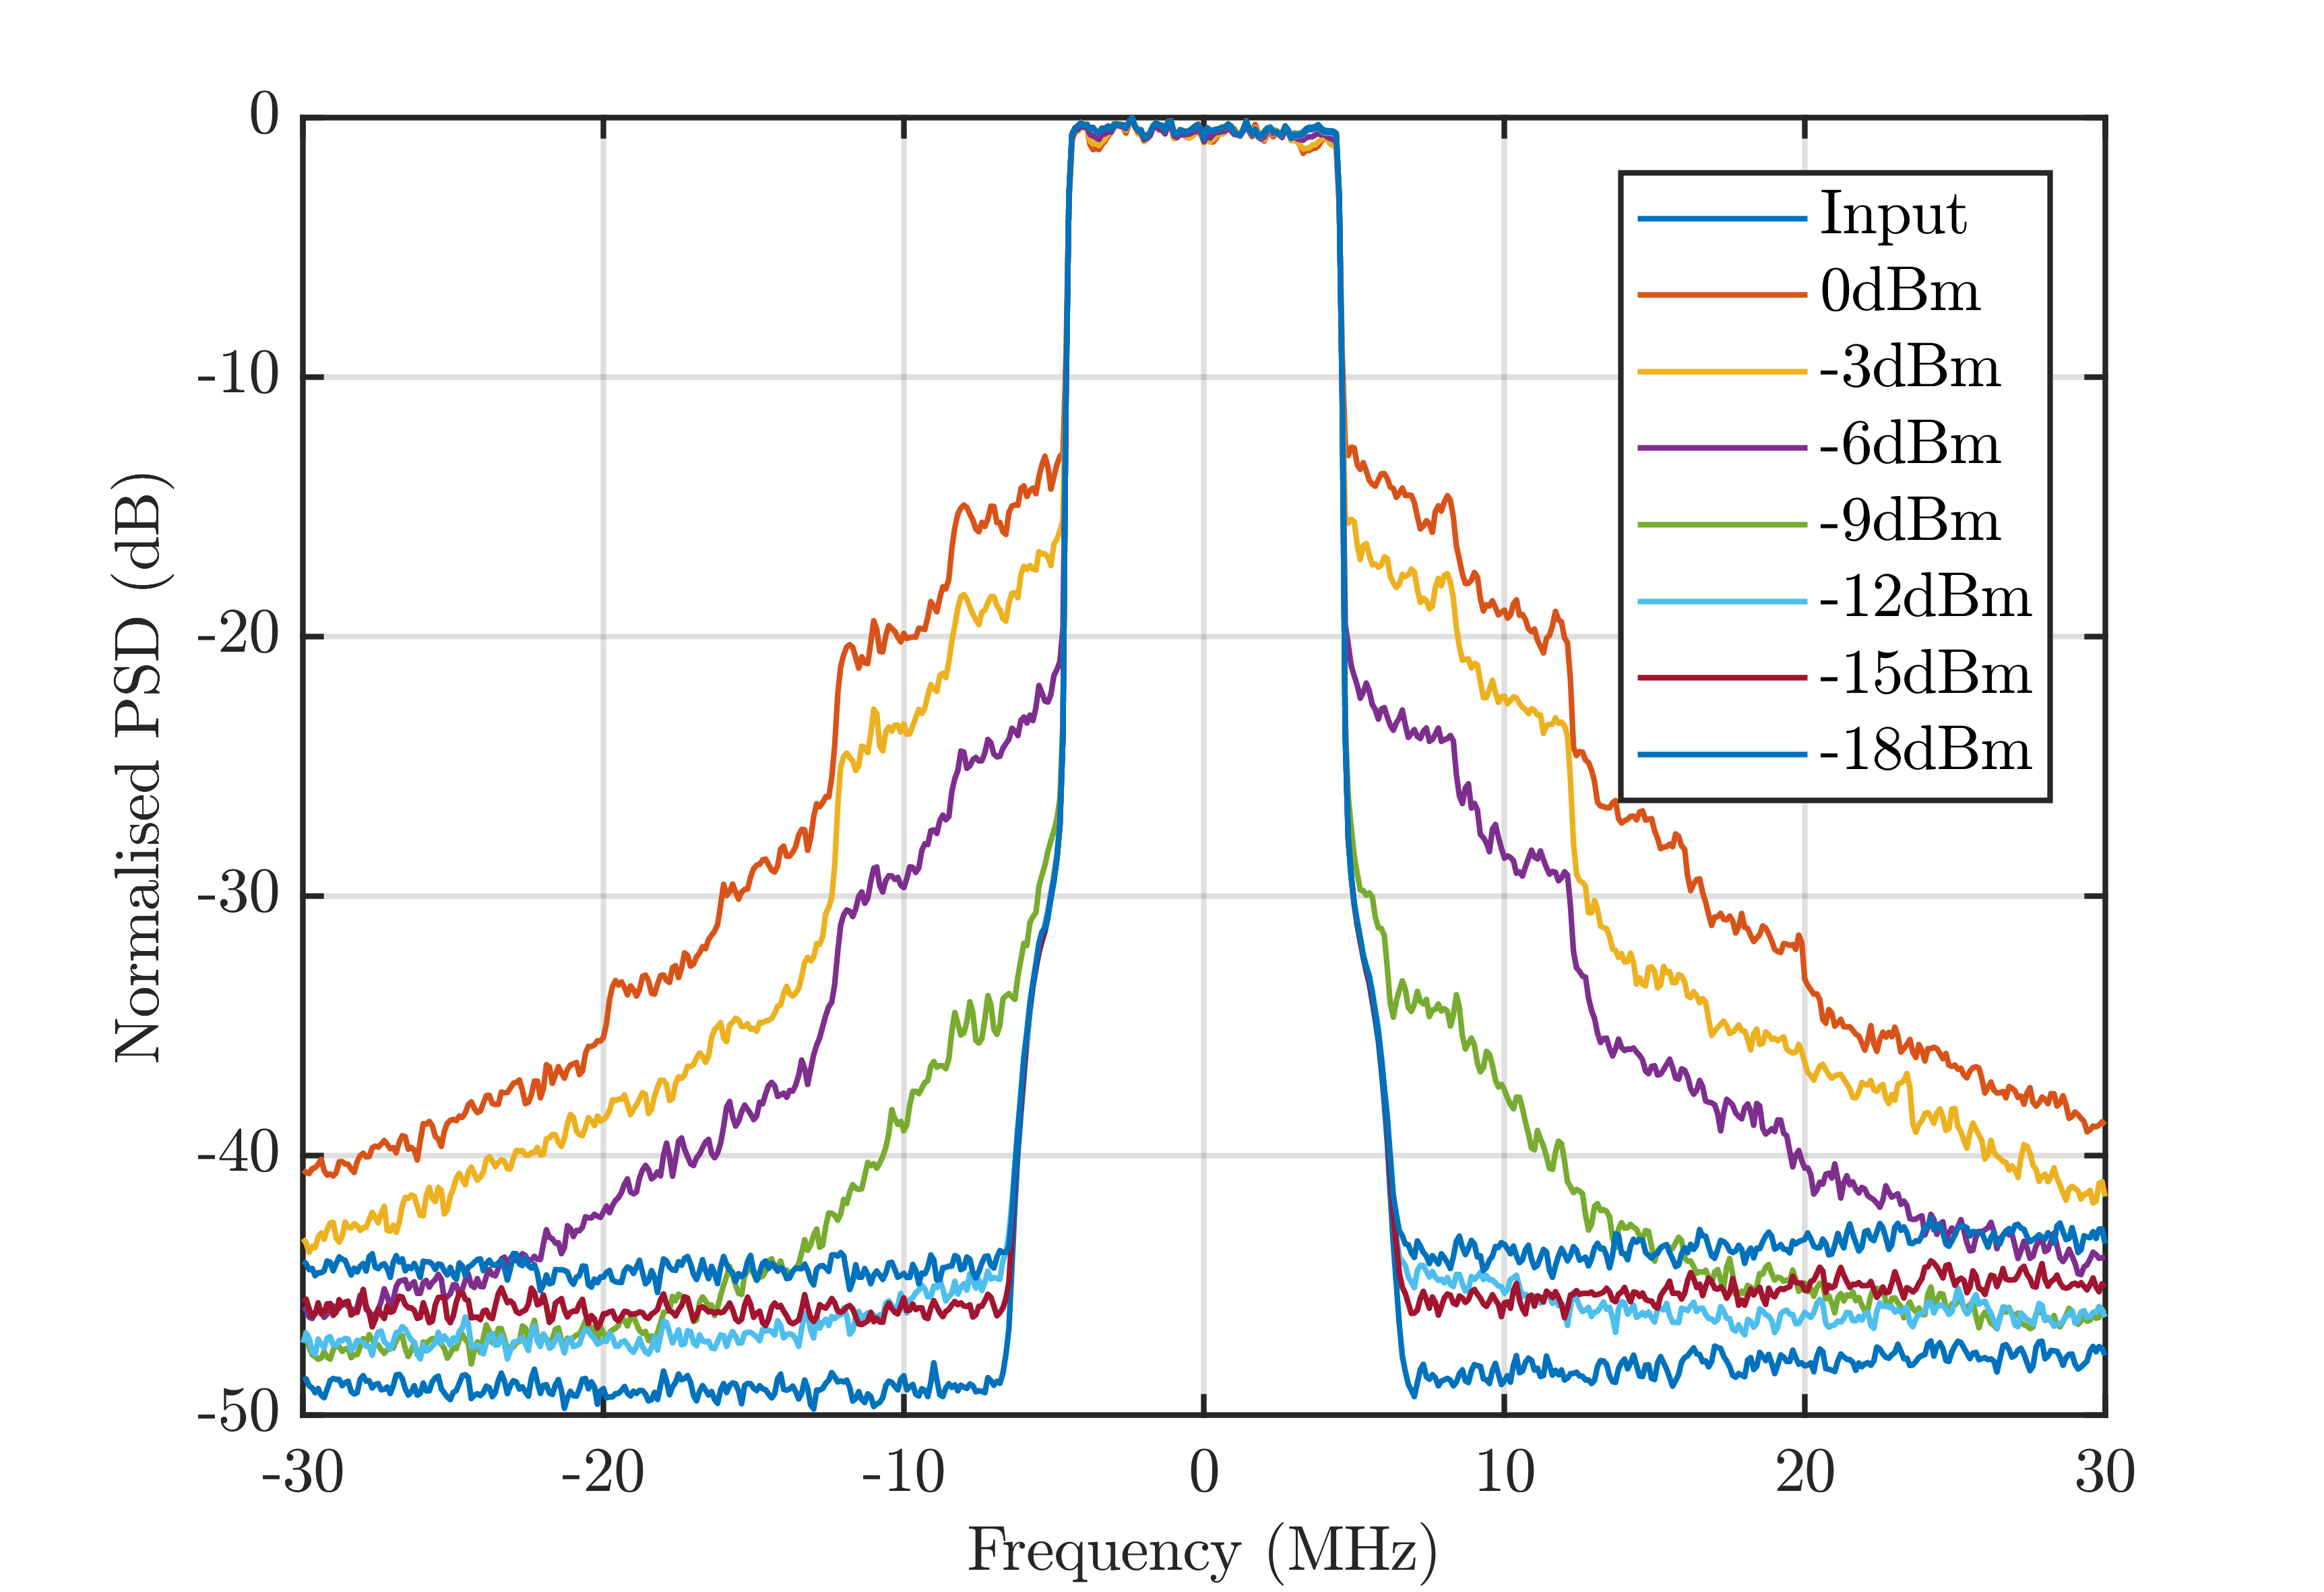
\includegraphics[scale = 0.5]{figures/measurement/four_antenna/psd_0p5.png}
	\caption{PSD at 0.5 $\lambda$ spacing between four antennas}
    \label{fig:psd05_4}
  \end{minipage}
  \hfill
  \begin{minipage}[b]{0.4\textwidth}
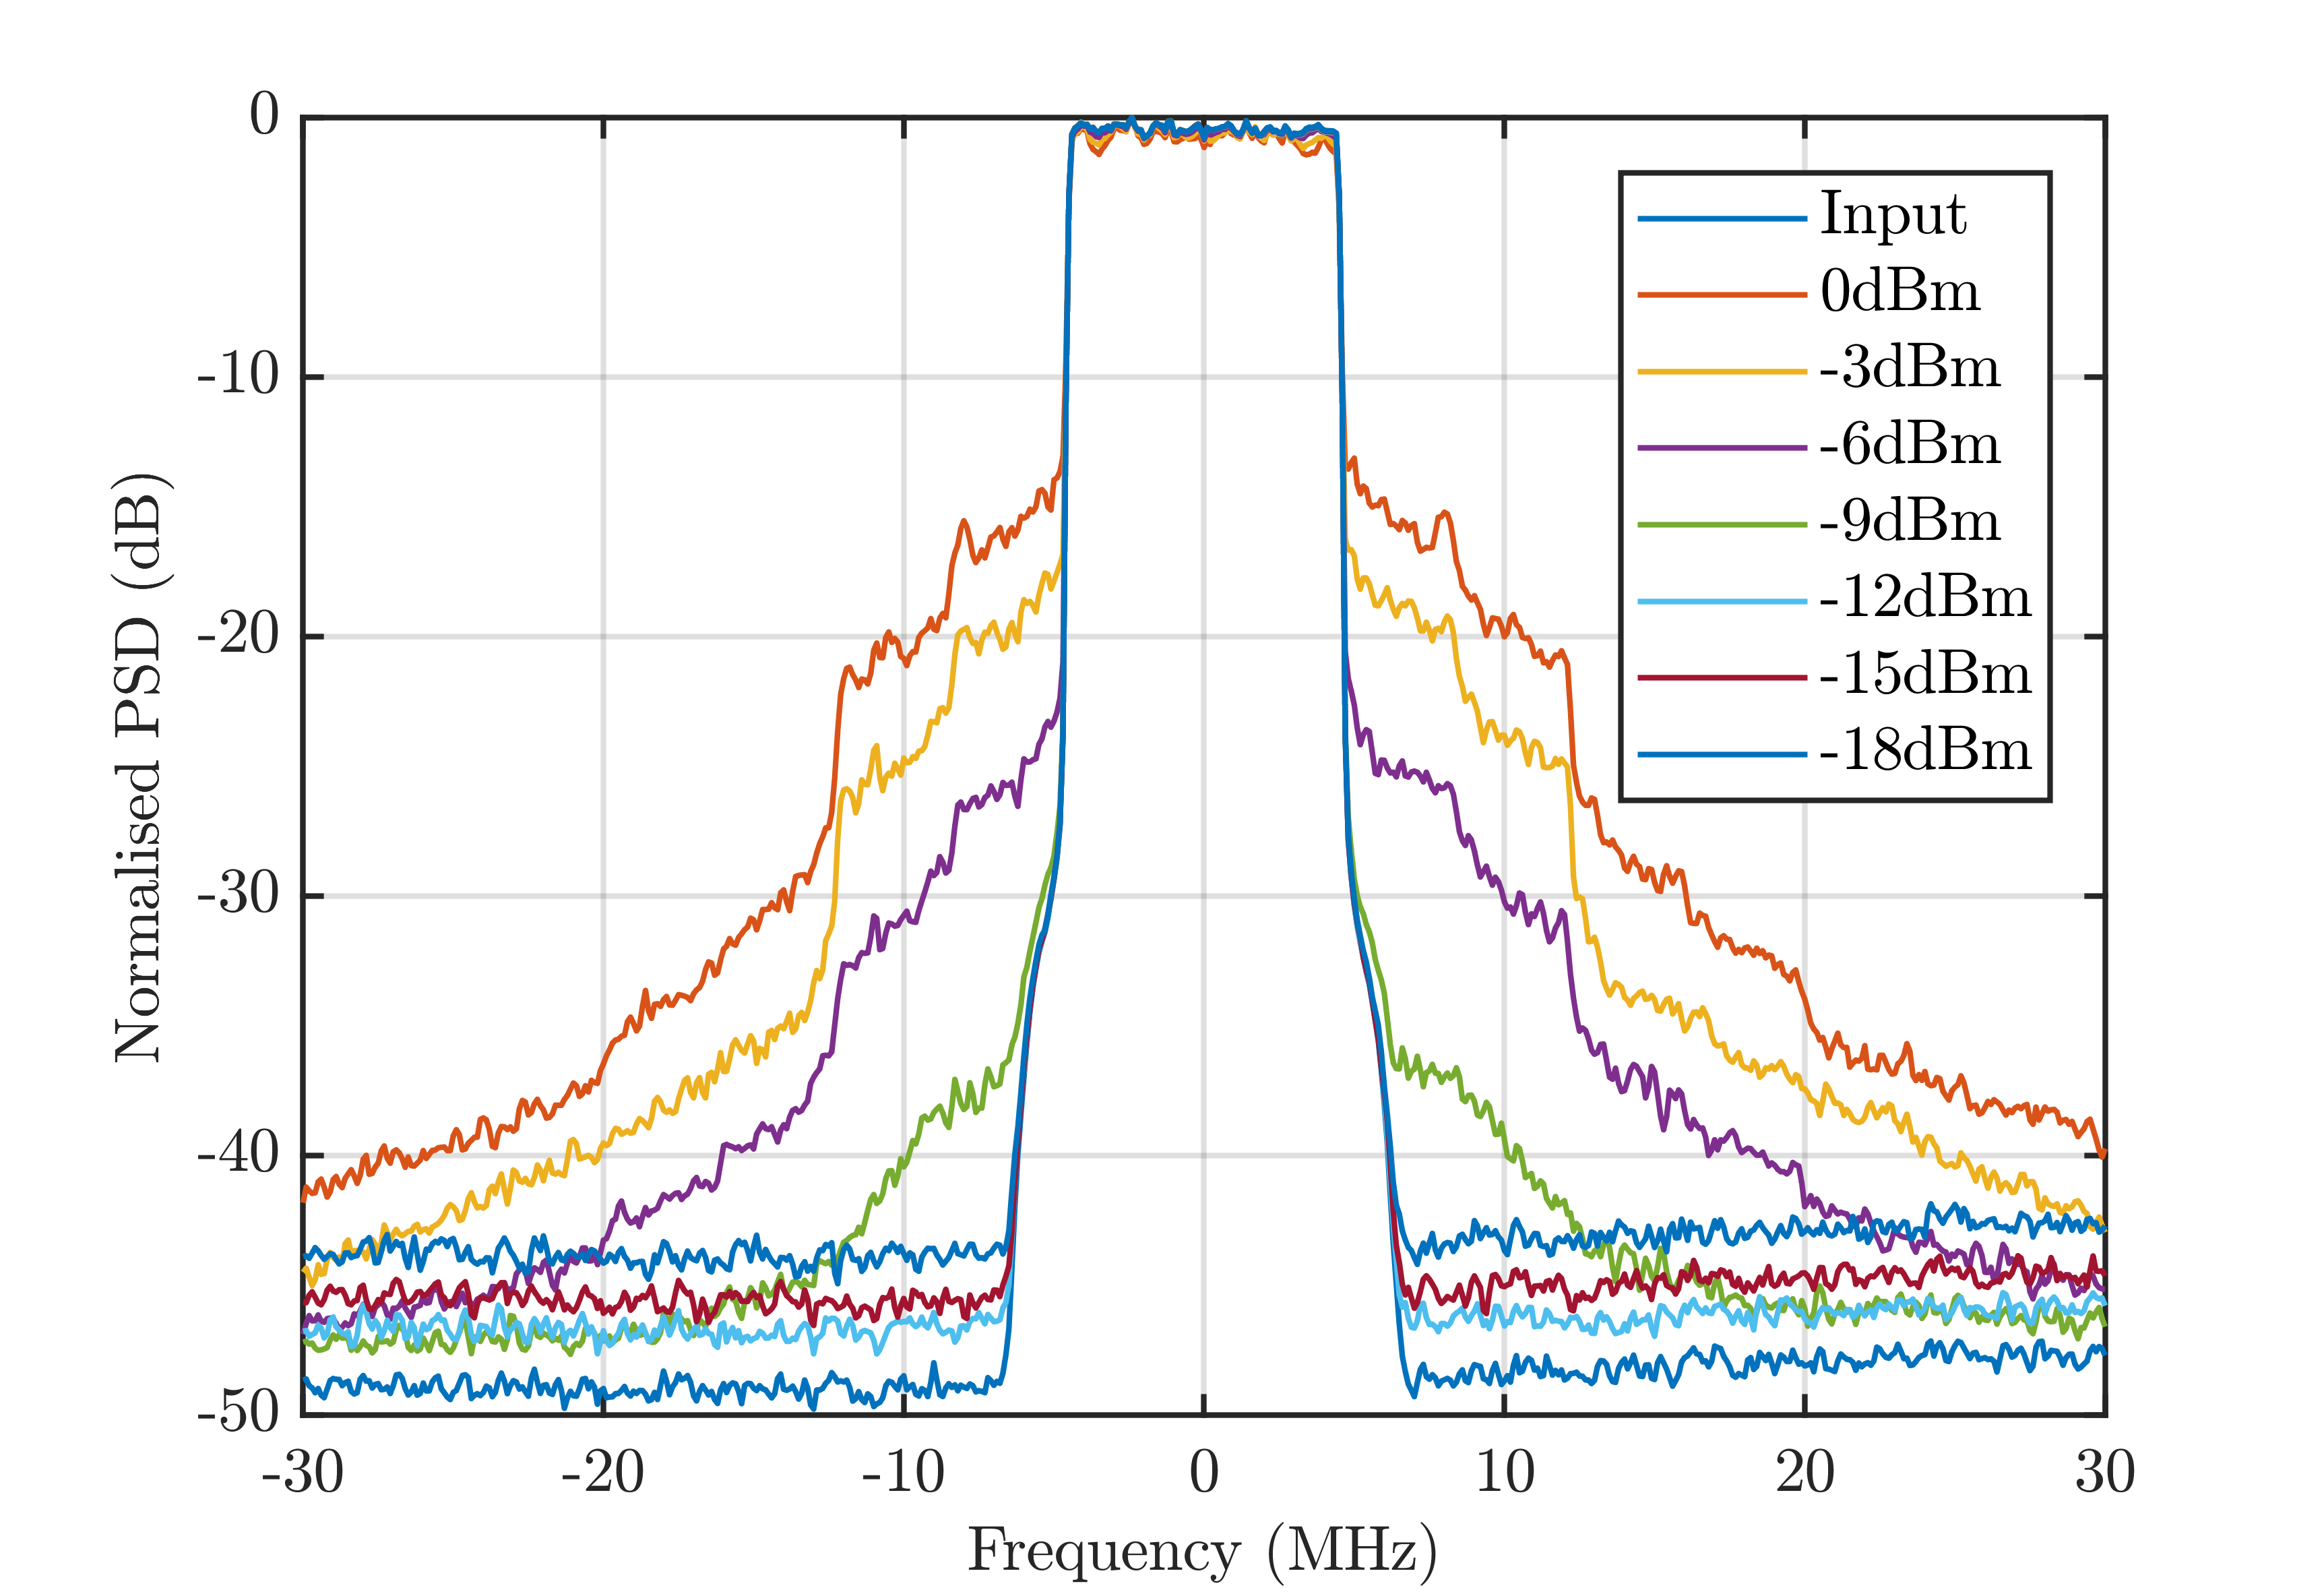
\includegraphics[scale = 0.5]{figures/measurement/four_antenna/psd_0p6.png}
\caption{PSD at 0.6 $\lambda$ spacing between four antennas}
    \label{fig:psd06_4}
  \end{minipage}
\end{figure}

\subsection{ACPR} %%%%%%%%%%%%%%%%%%%%%%%%%%%%%%%%%%%%%%%%%%%%%%%%%%%%%%%%%%%%%%%%%%%%%%%%%%%%%%%%%%%%%%%%%%%%%%%

\subsubsection{Two transmit antenna}

\begin{figure}[H]
\centering 
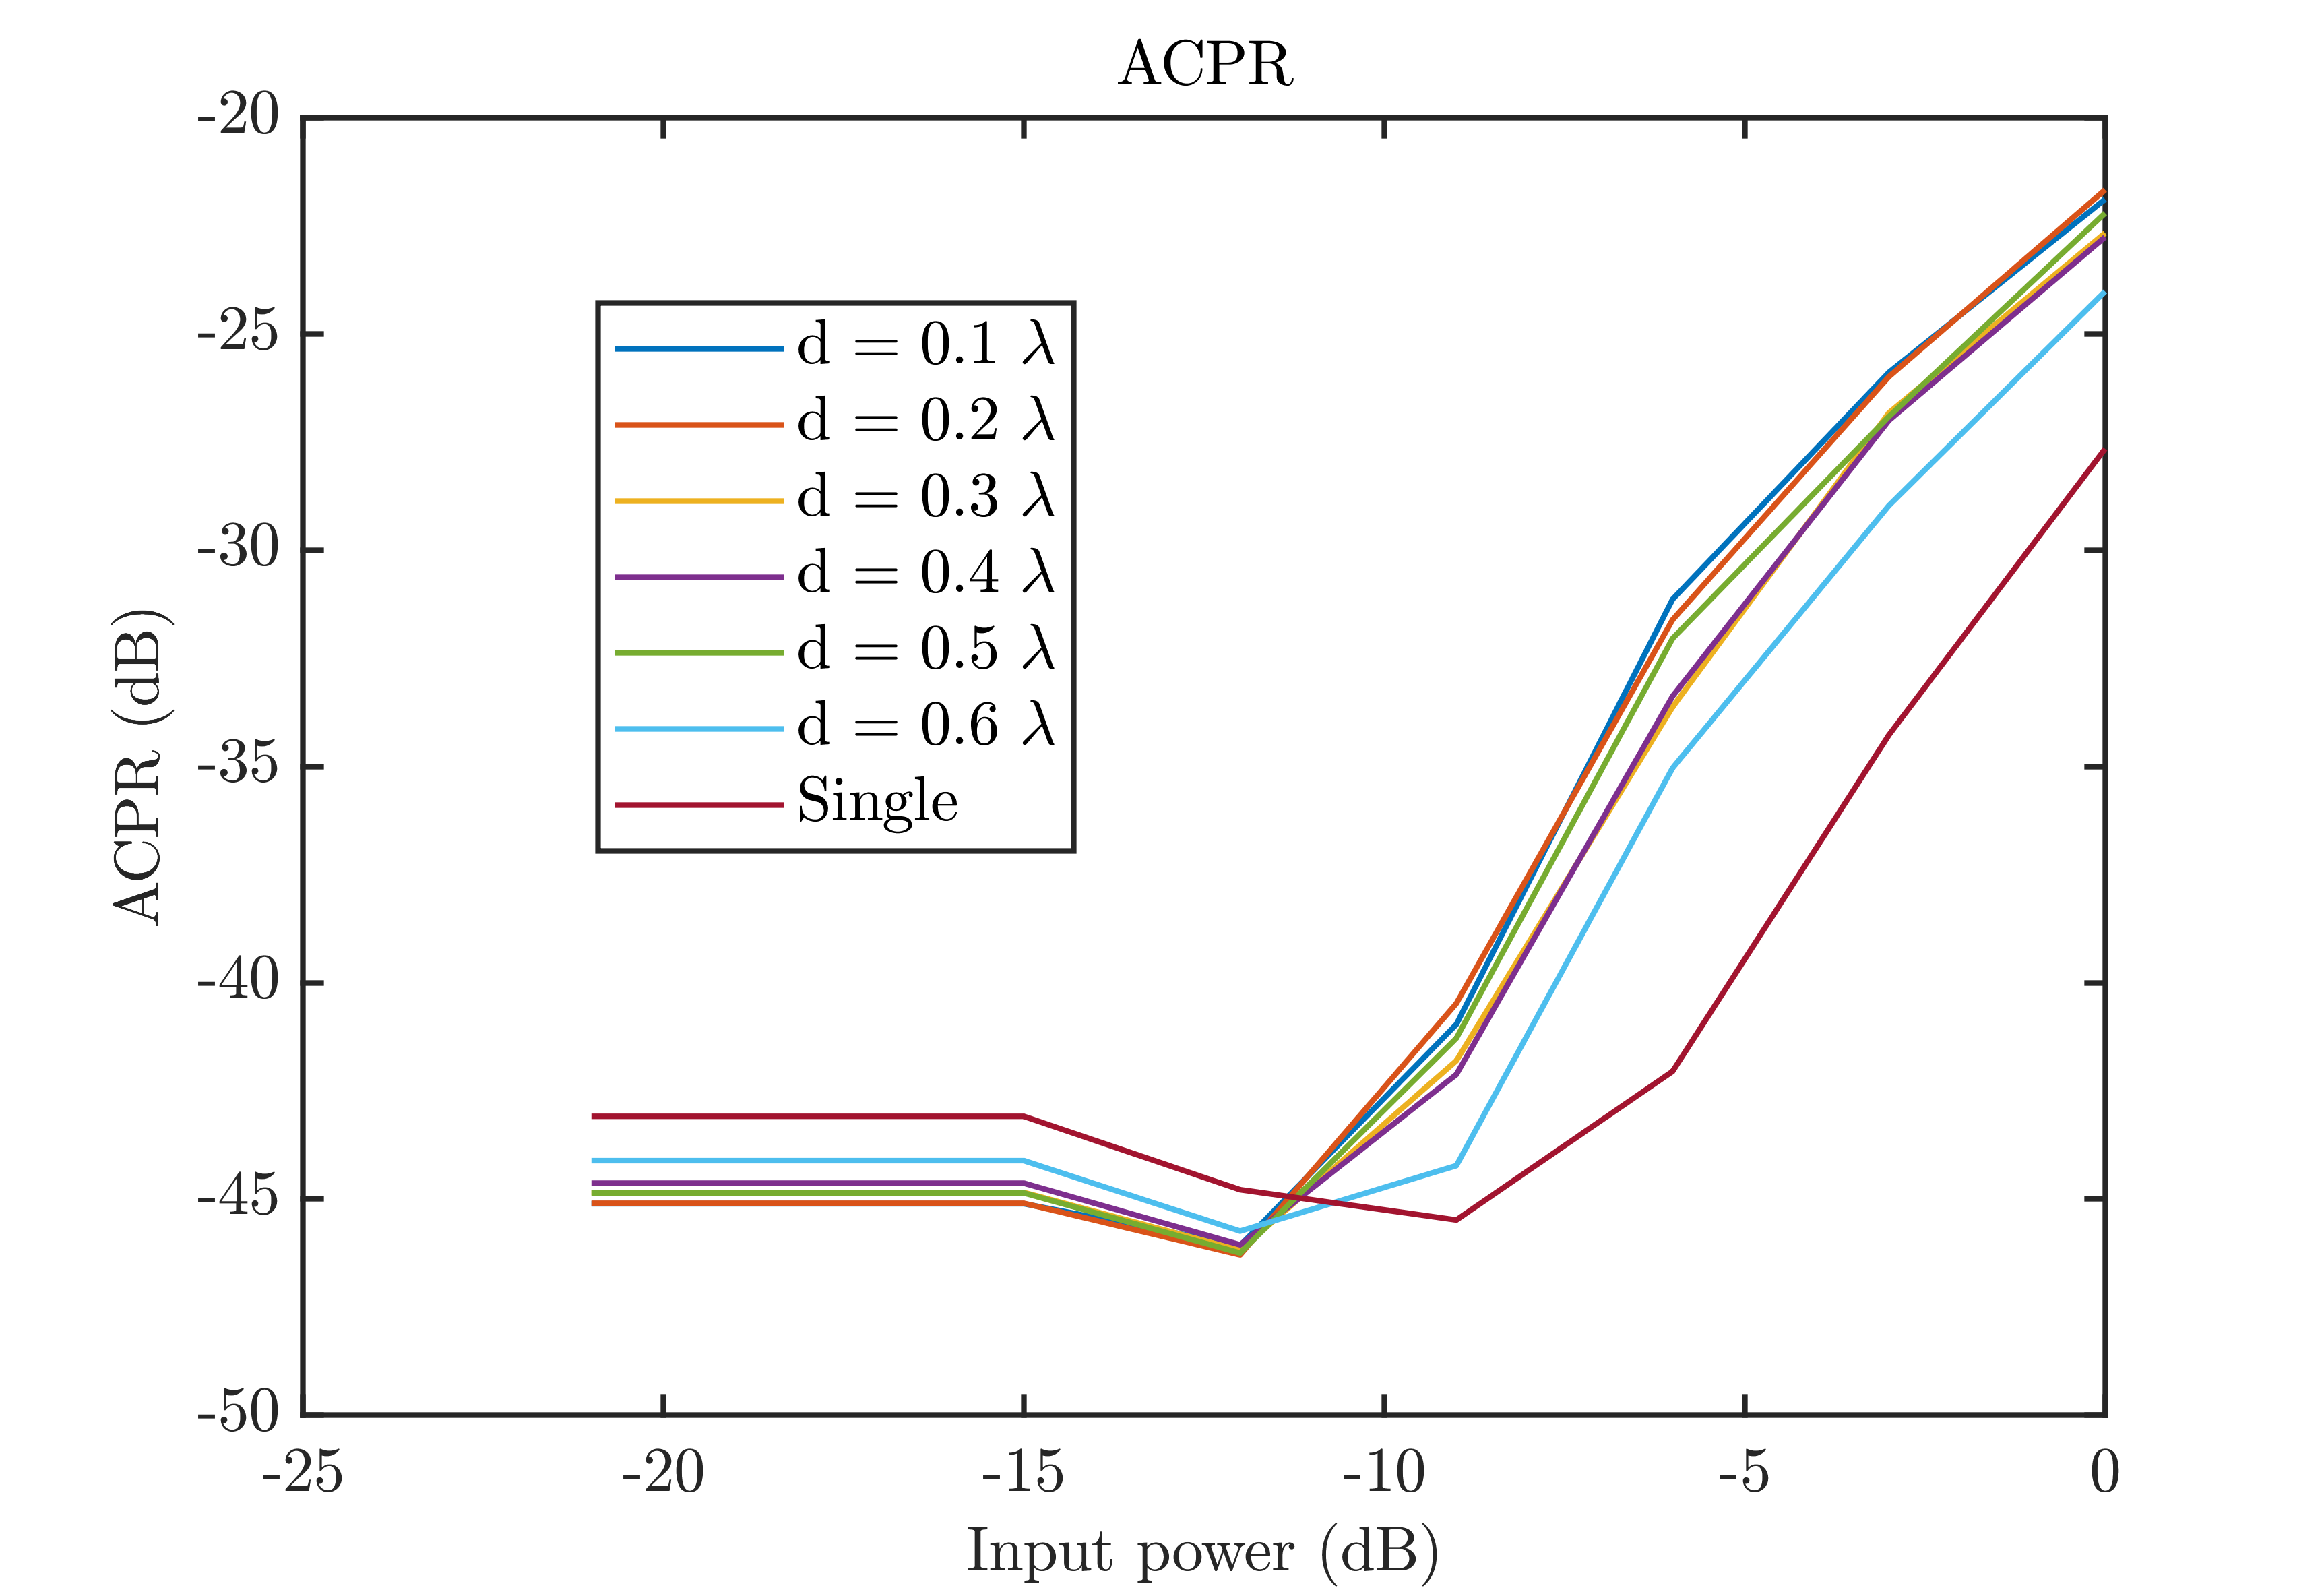
\includegraphics[scale = 1]{figures/measurement/two_antenna/ACPR.png}
\caption{ACPR using two transmit antennas}
\label{fig:acpr_meas1}
\end{figure} 

\subsubsection{Four transmit antenna}

\begin{figure}[H]
\centering 
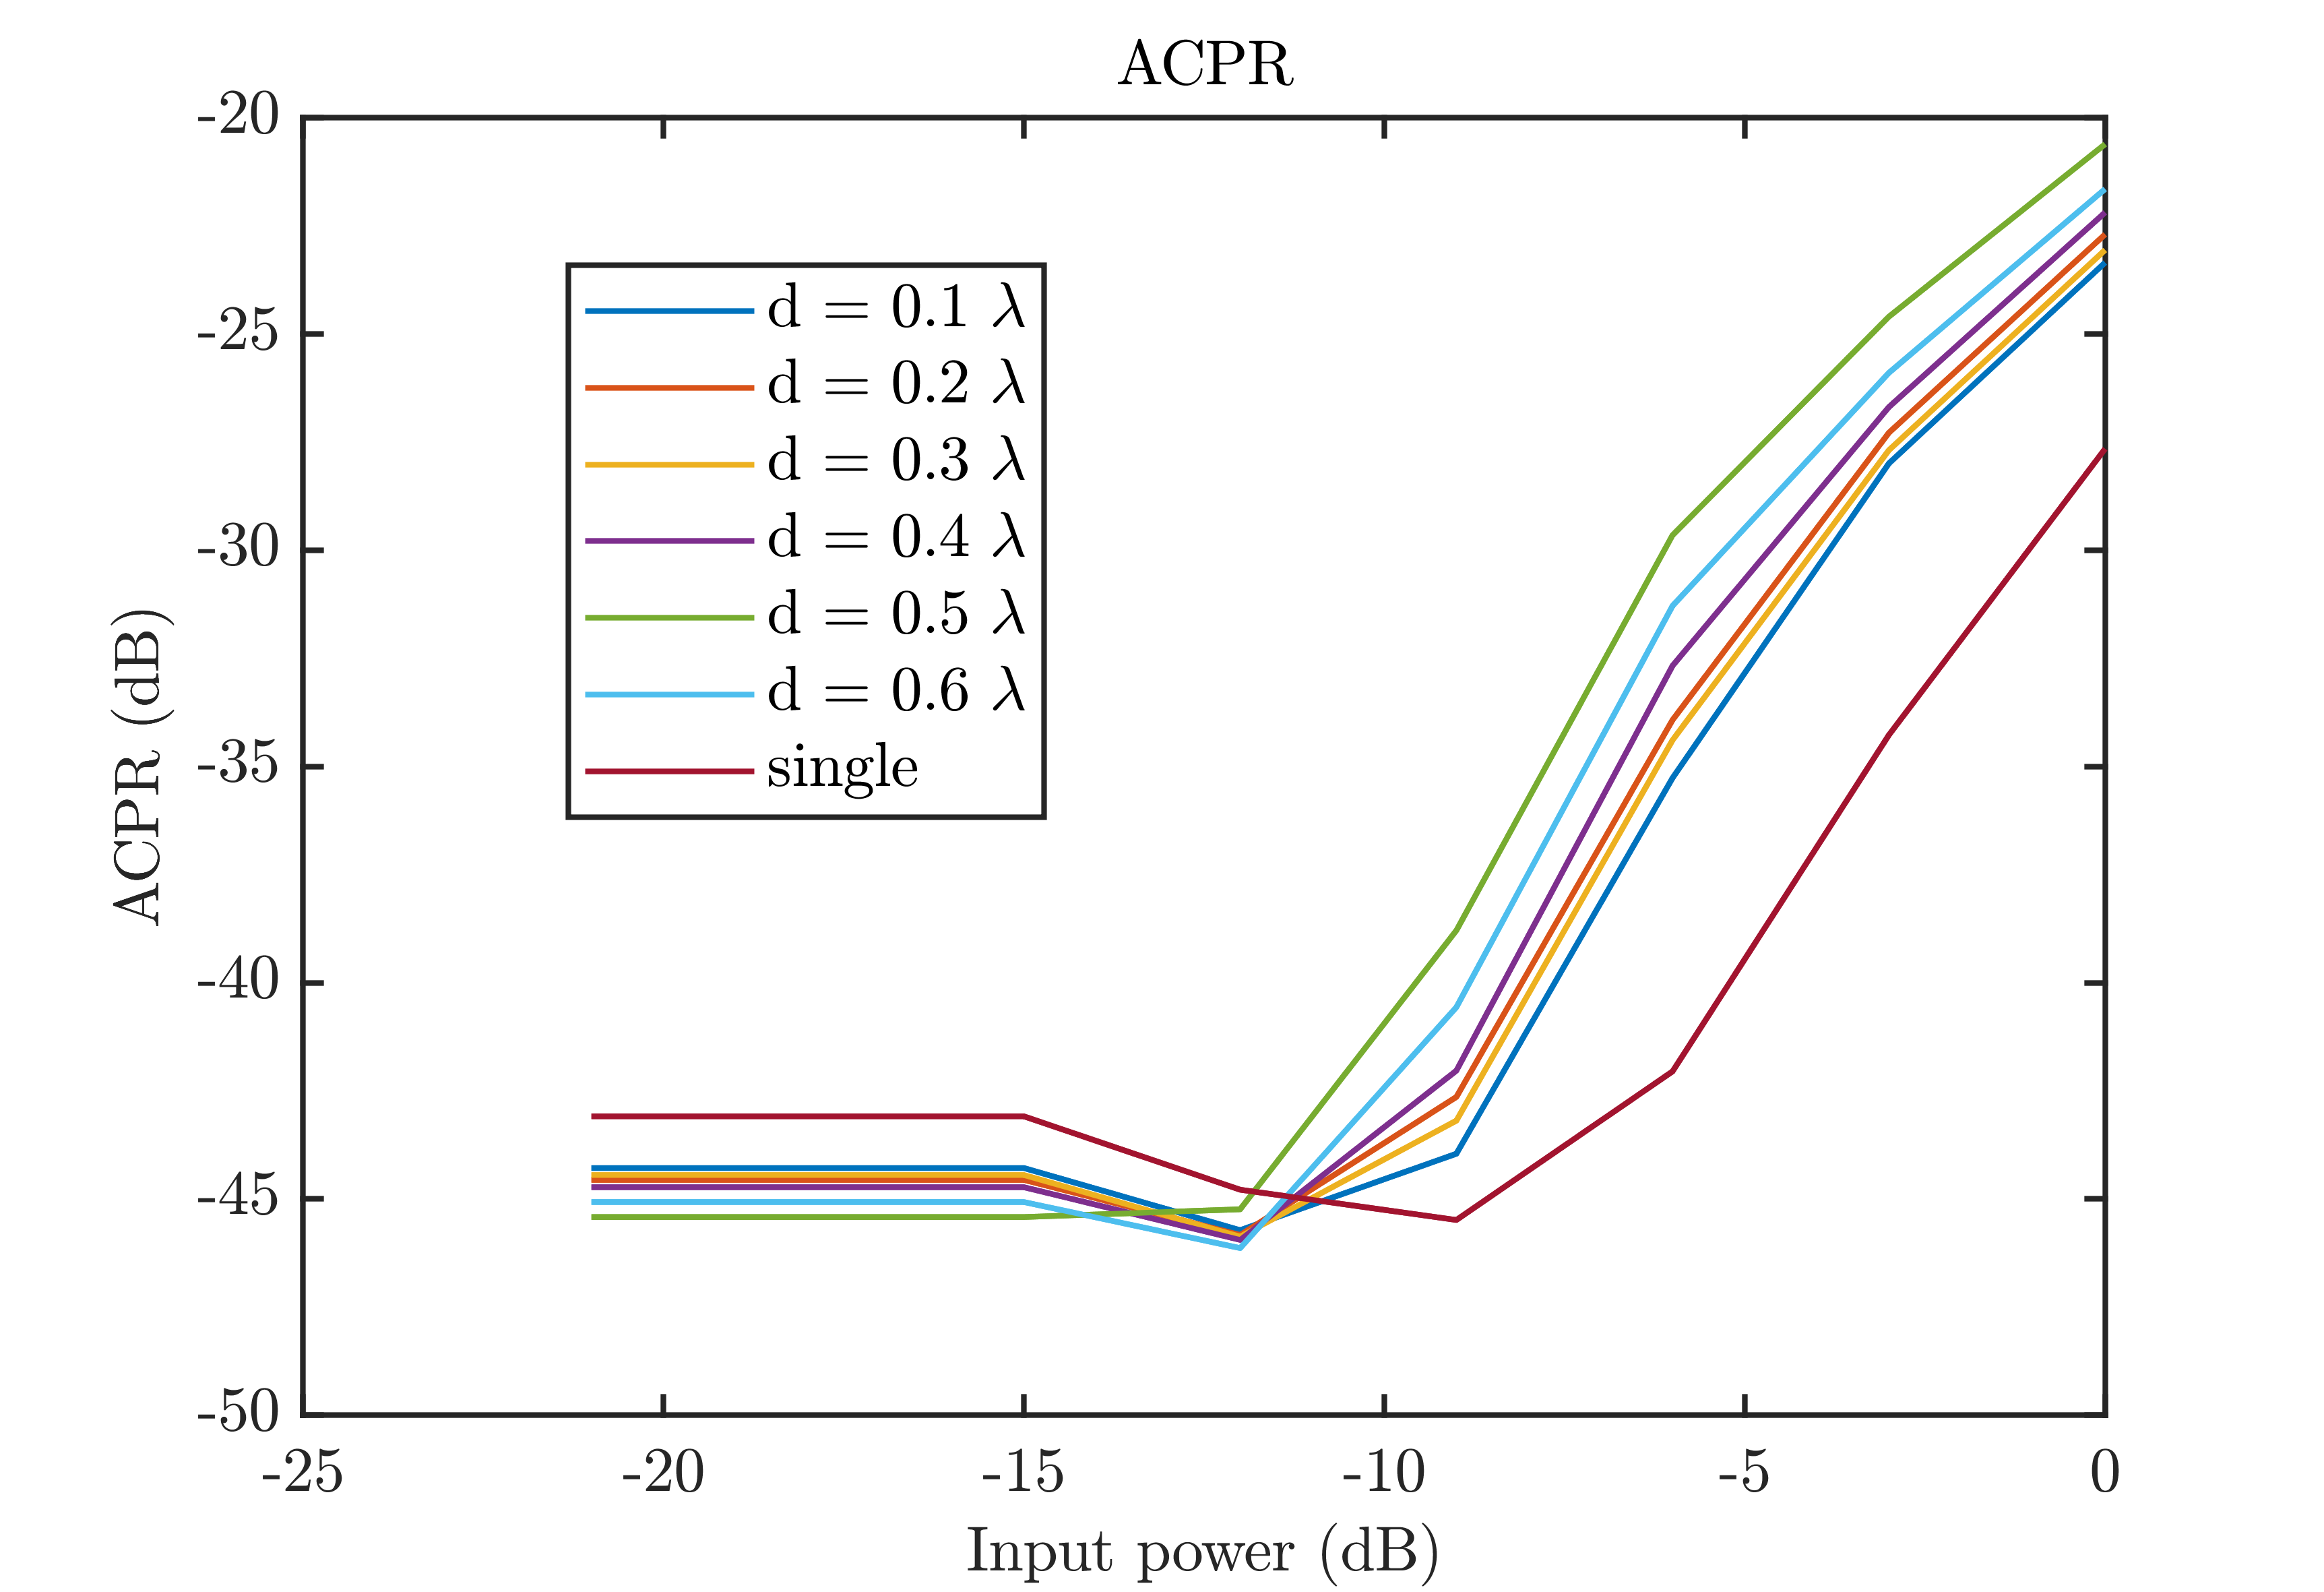
\includegraphics[scale = 1]{figures/measurement/four_antenna/ACPR.png}
\caption{ACPR using four transmit antennas}
\label{fig:acpr_meas2}
\end{figure} 

\todo[inline]{lav figur med -dbm input ved forskellige afstande}


%%%%%%%%%%%%%%%%%%%%%%%%%%%%%%%%%%%%%%%%%%%%%%%%%%%%%%%%%%%%%%%%%%%%%%%%%%%%%%%%%%%%%%%%%%%%%%%%%%%%%%%%%%%%%%%%%%

\section{Measurement setup 2}

\subsubsection{Amplifier only}

In this section an other amplifier has been used.....

First step is to measure the amplifier and find the input level where the amplifier compresses and then do the DPD. 

\begin{figure}[H]
\centering 
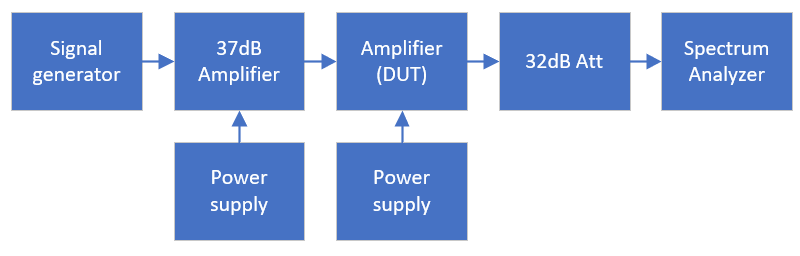
\includegraphics[scale = 0.5]{figures/measurement/meas_set_cree_1.png}
\caption{Measurement setup}
\label{fig:meas2_cree1}
\end{figure} 

\begin{figure}[H]
  \centering
  \begin{minipage}[b]{0.5\textwidth}
	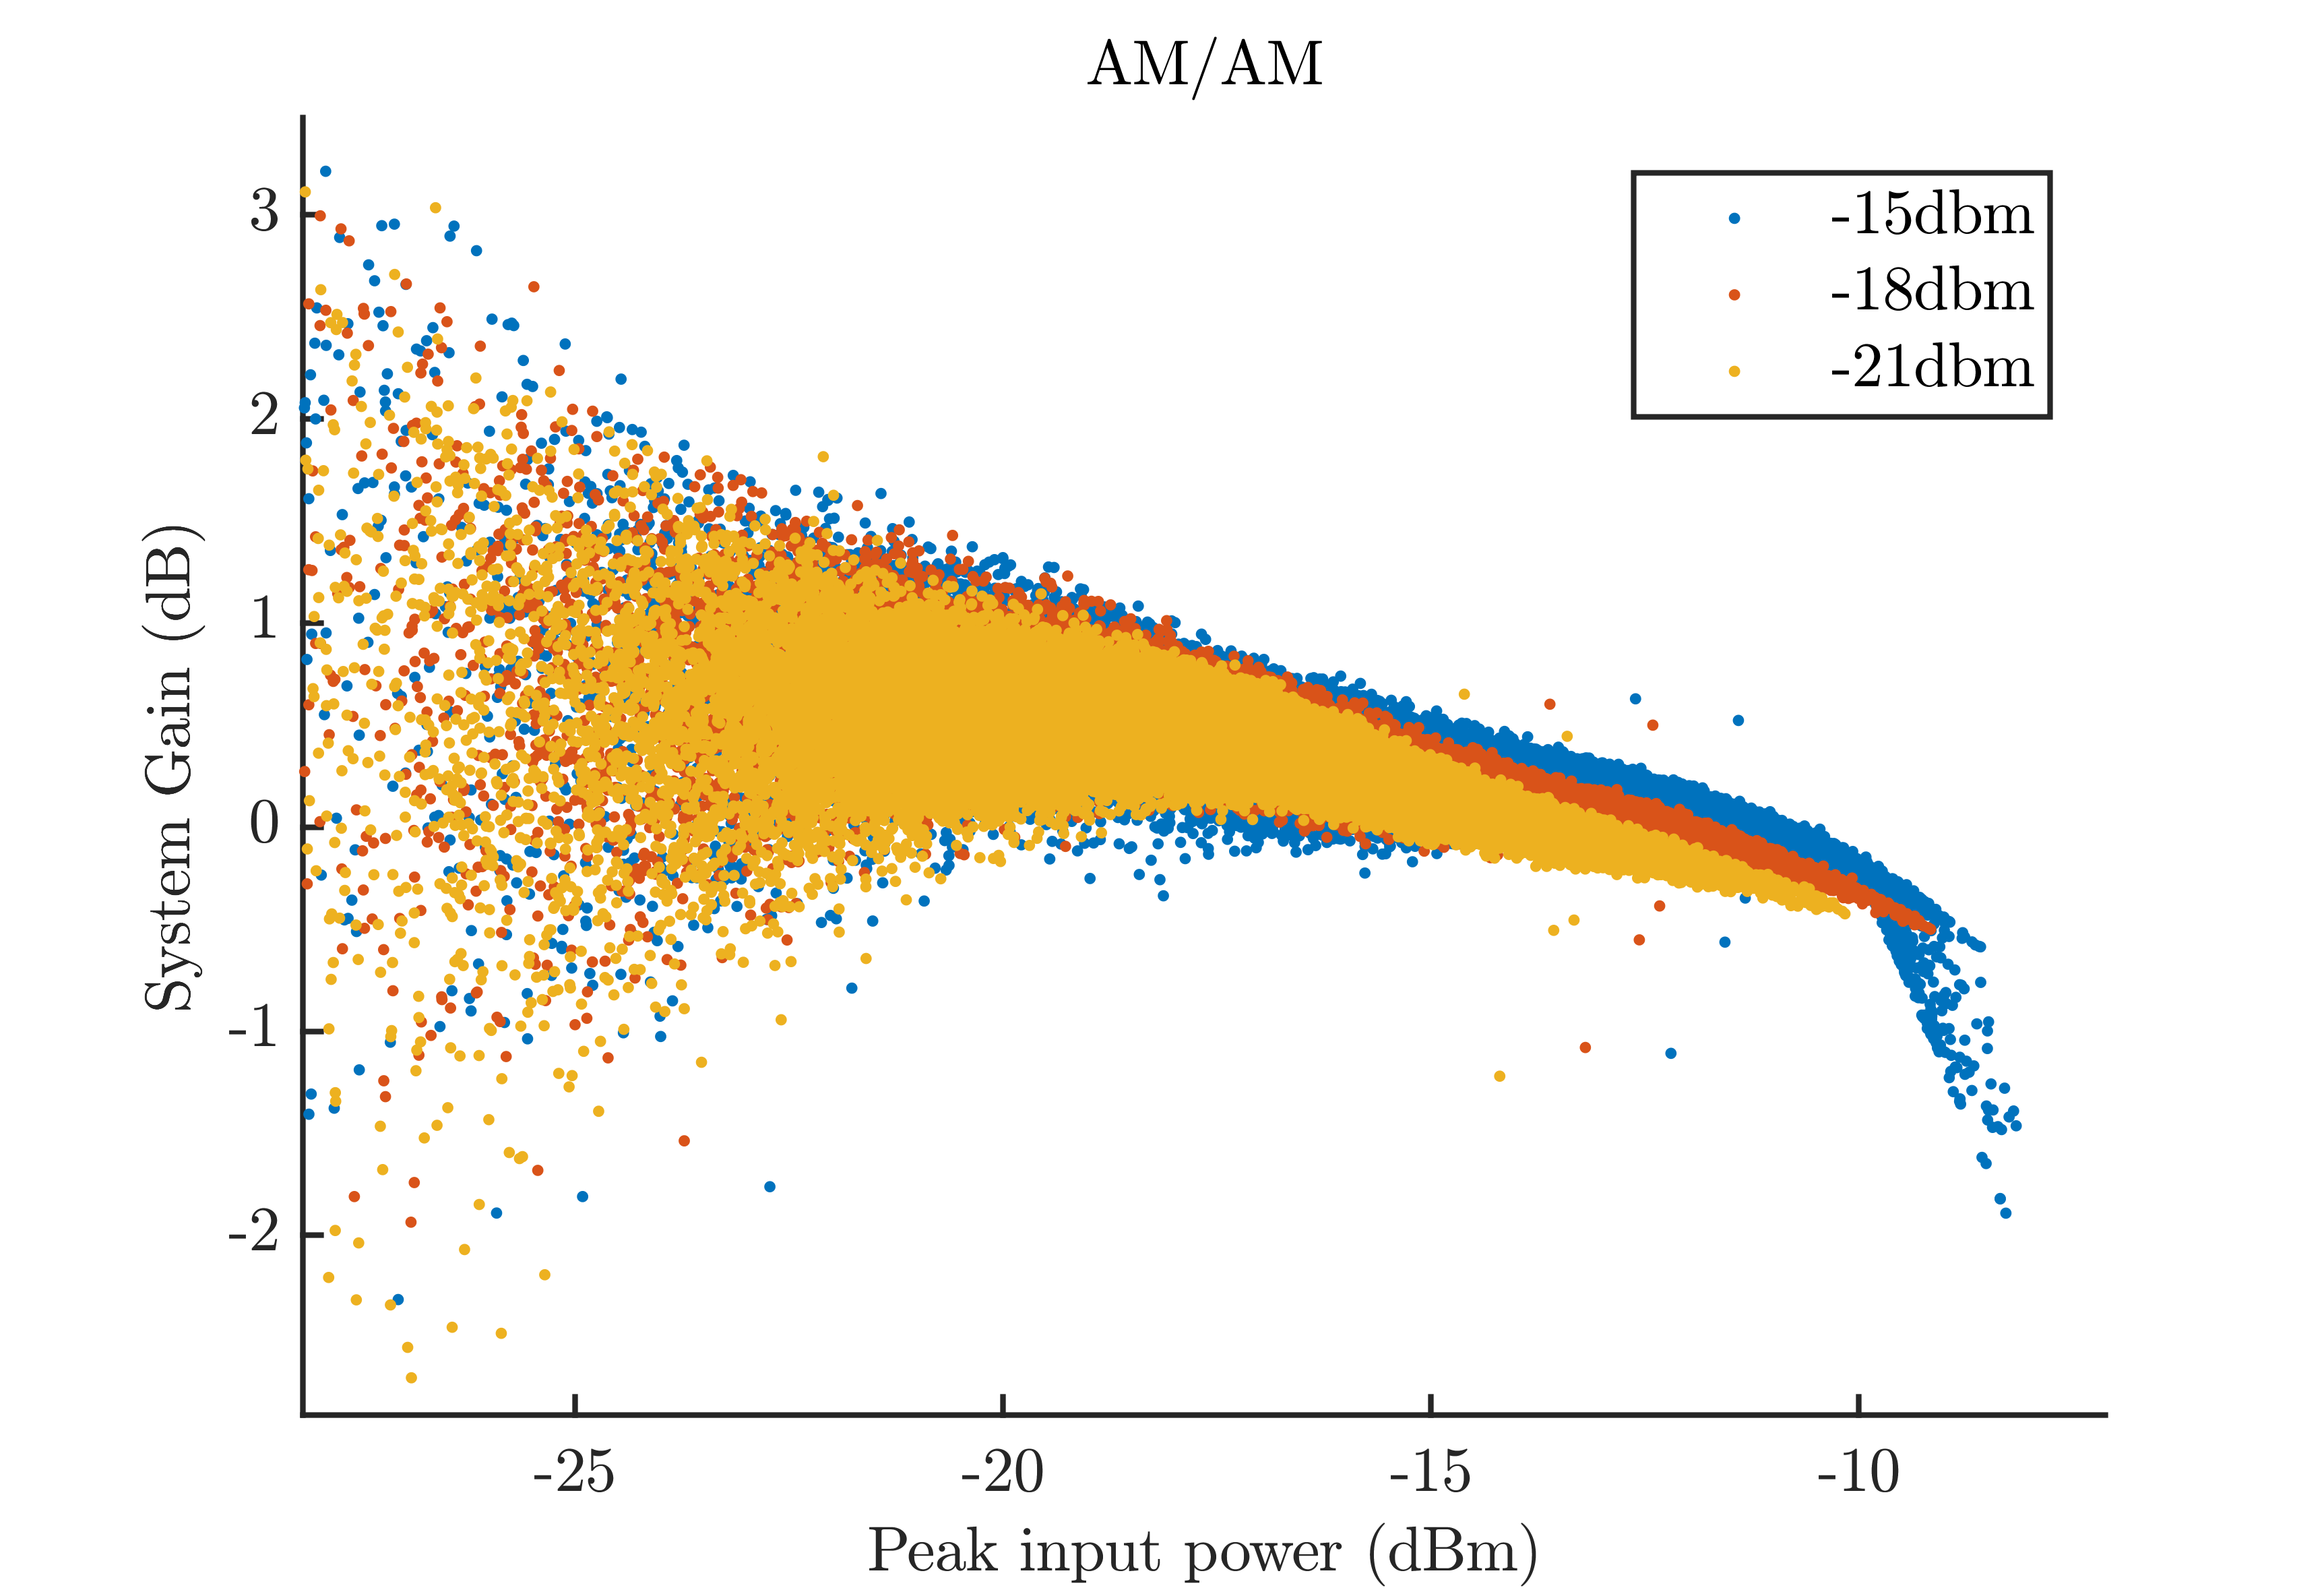
\includegraphics[scale = 0.5]{figures/measurement/cree/amam_cree_amp_no_dpd.png}
	\caption{AM/AM of amplifier}
    \label{fig:cree_amam1}
  \end{minipage}
  \hfill
  \begin{minipage}[b]{0.4\textwidth}
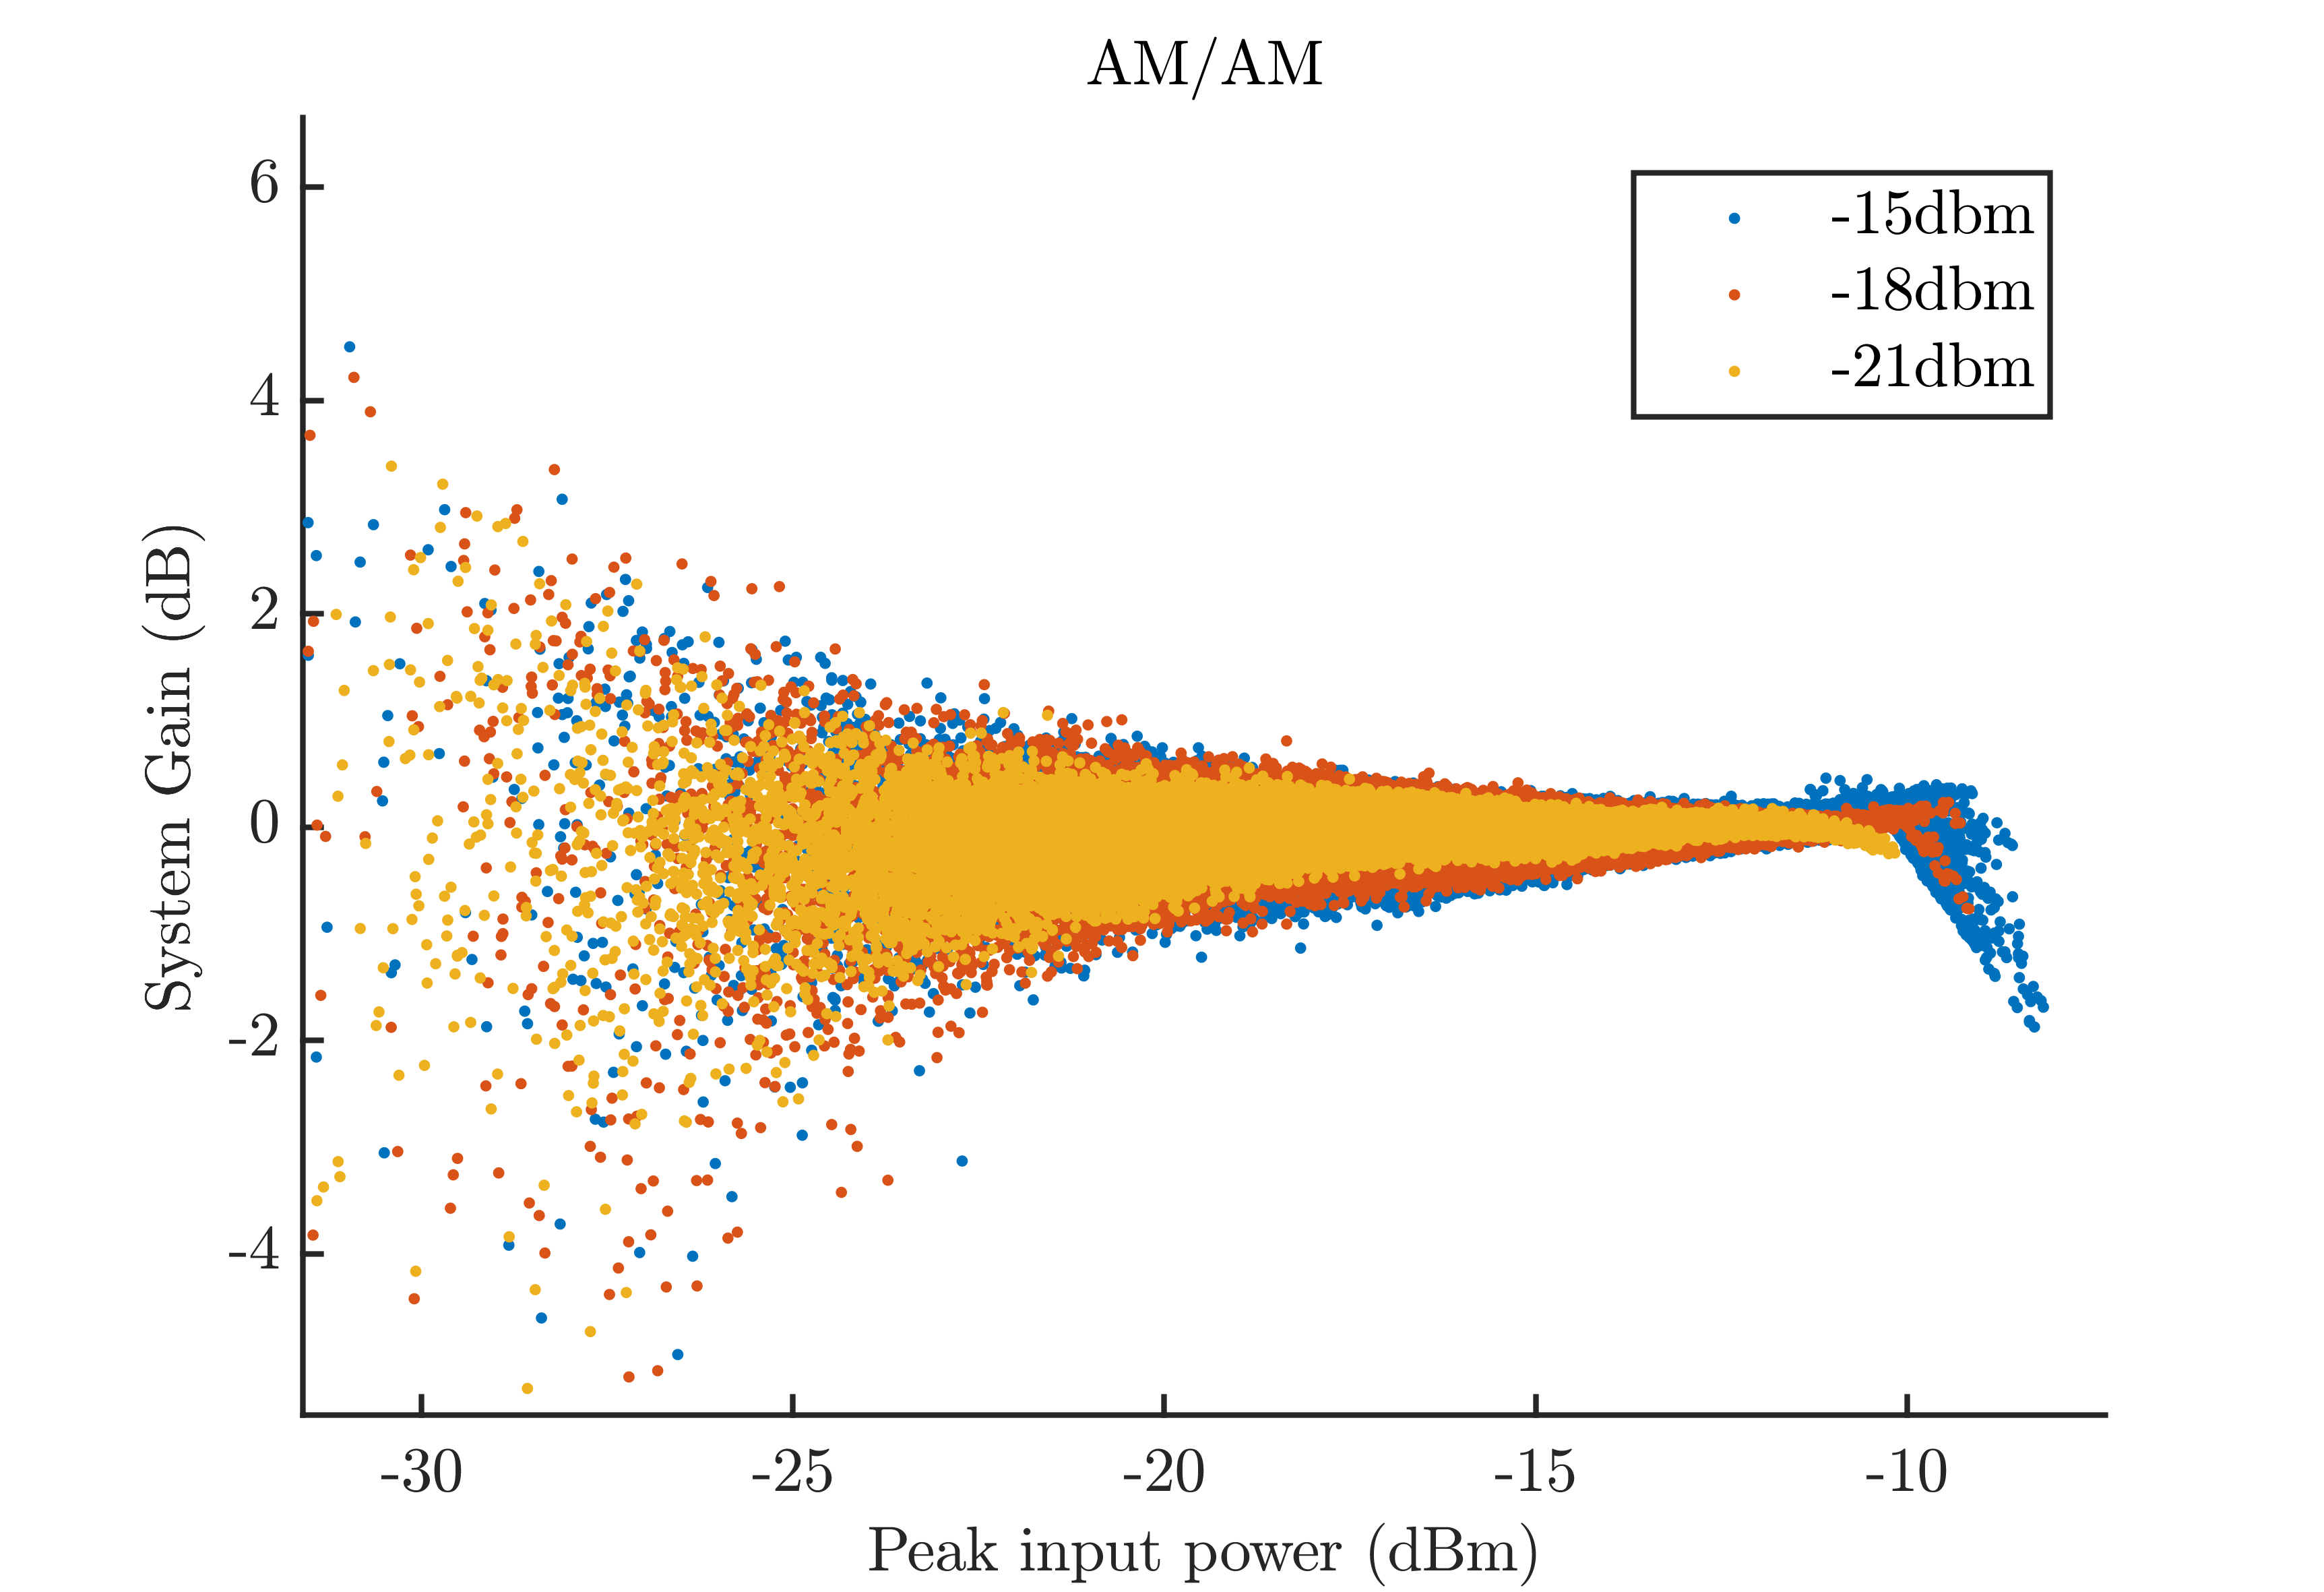
\includegraphics[scale = 0.5]{figures/measurement/cree/amam_cree_amp_with_dpd.png}
\caption{AM/AM of amplifier with DPD}
    \label{fig:cree_amam2}
  \end{minipage}
\end{figure}


\begin{figure}[H]
  \centering
  \begin{minipage}[b]{0.5\textwidth}
	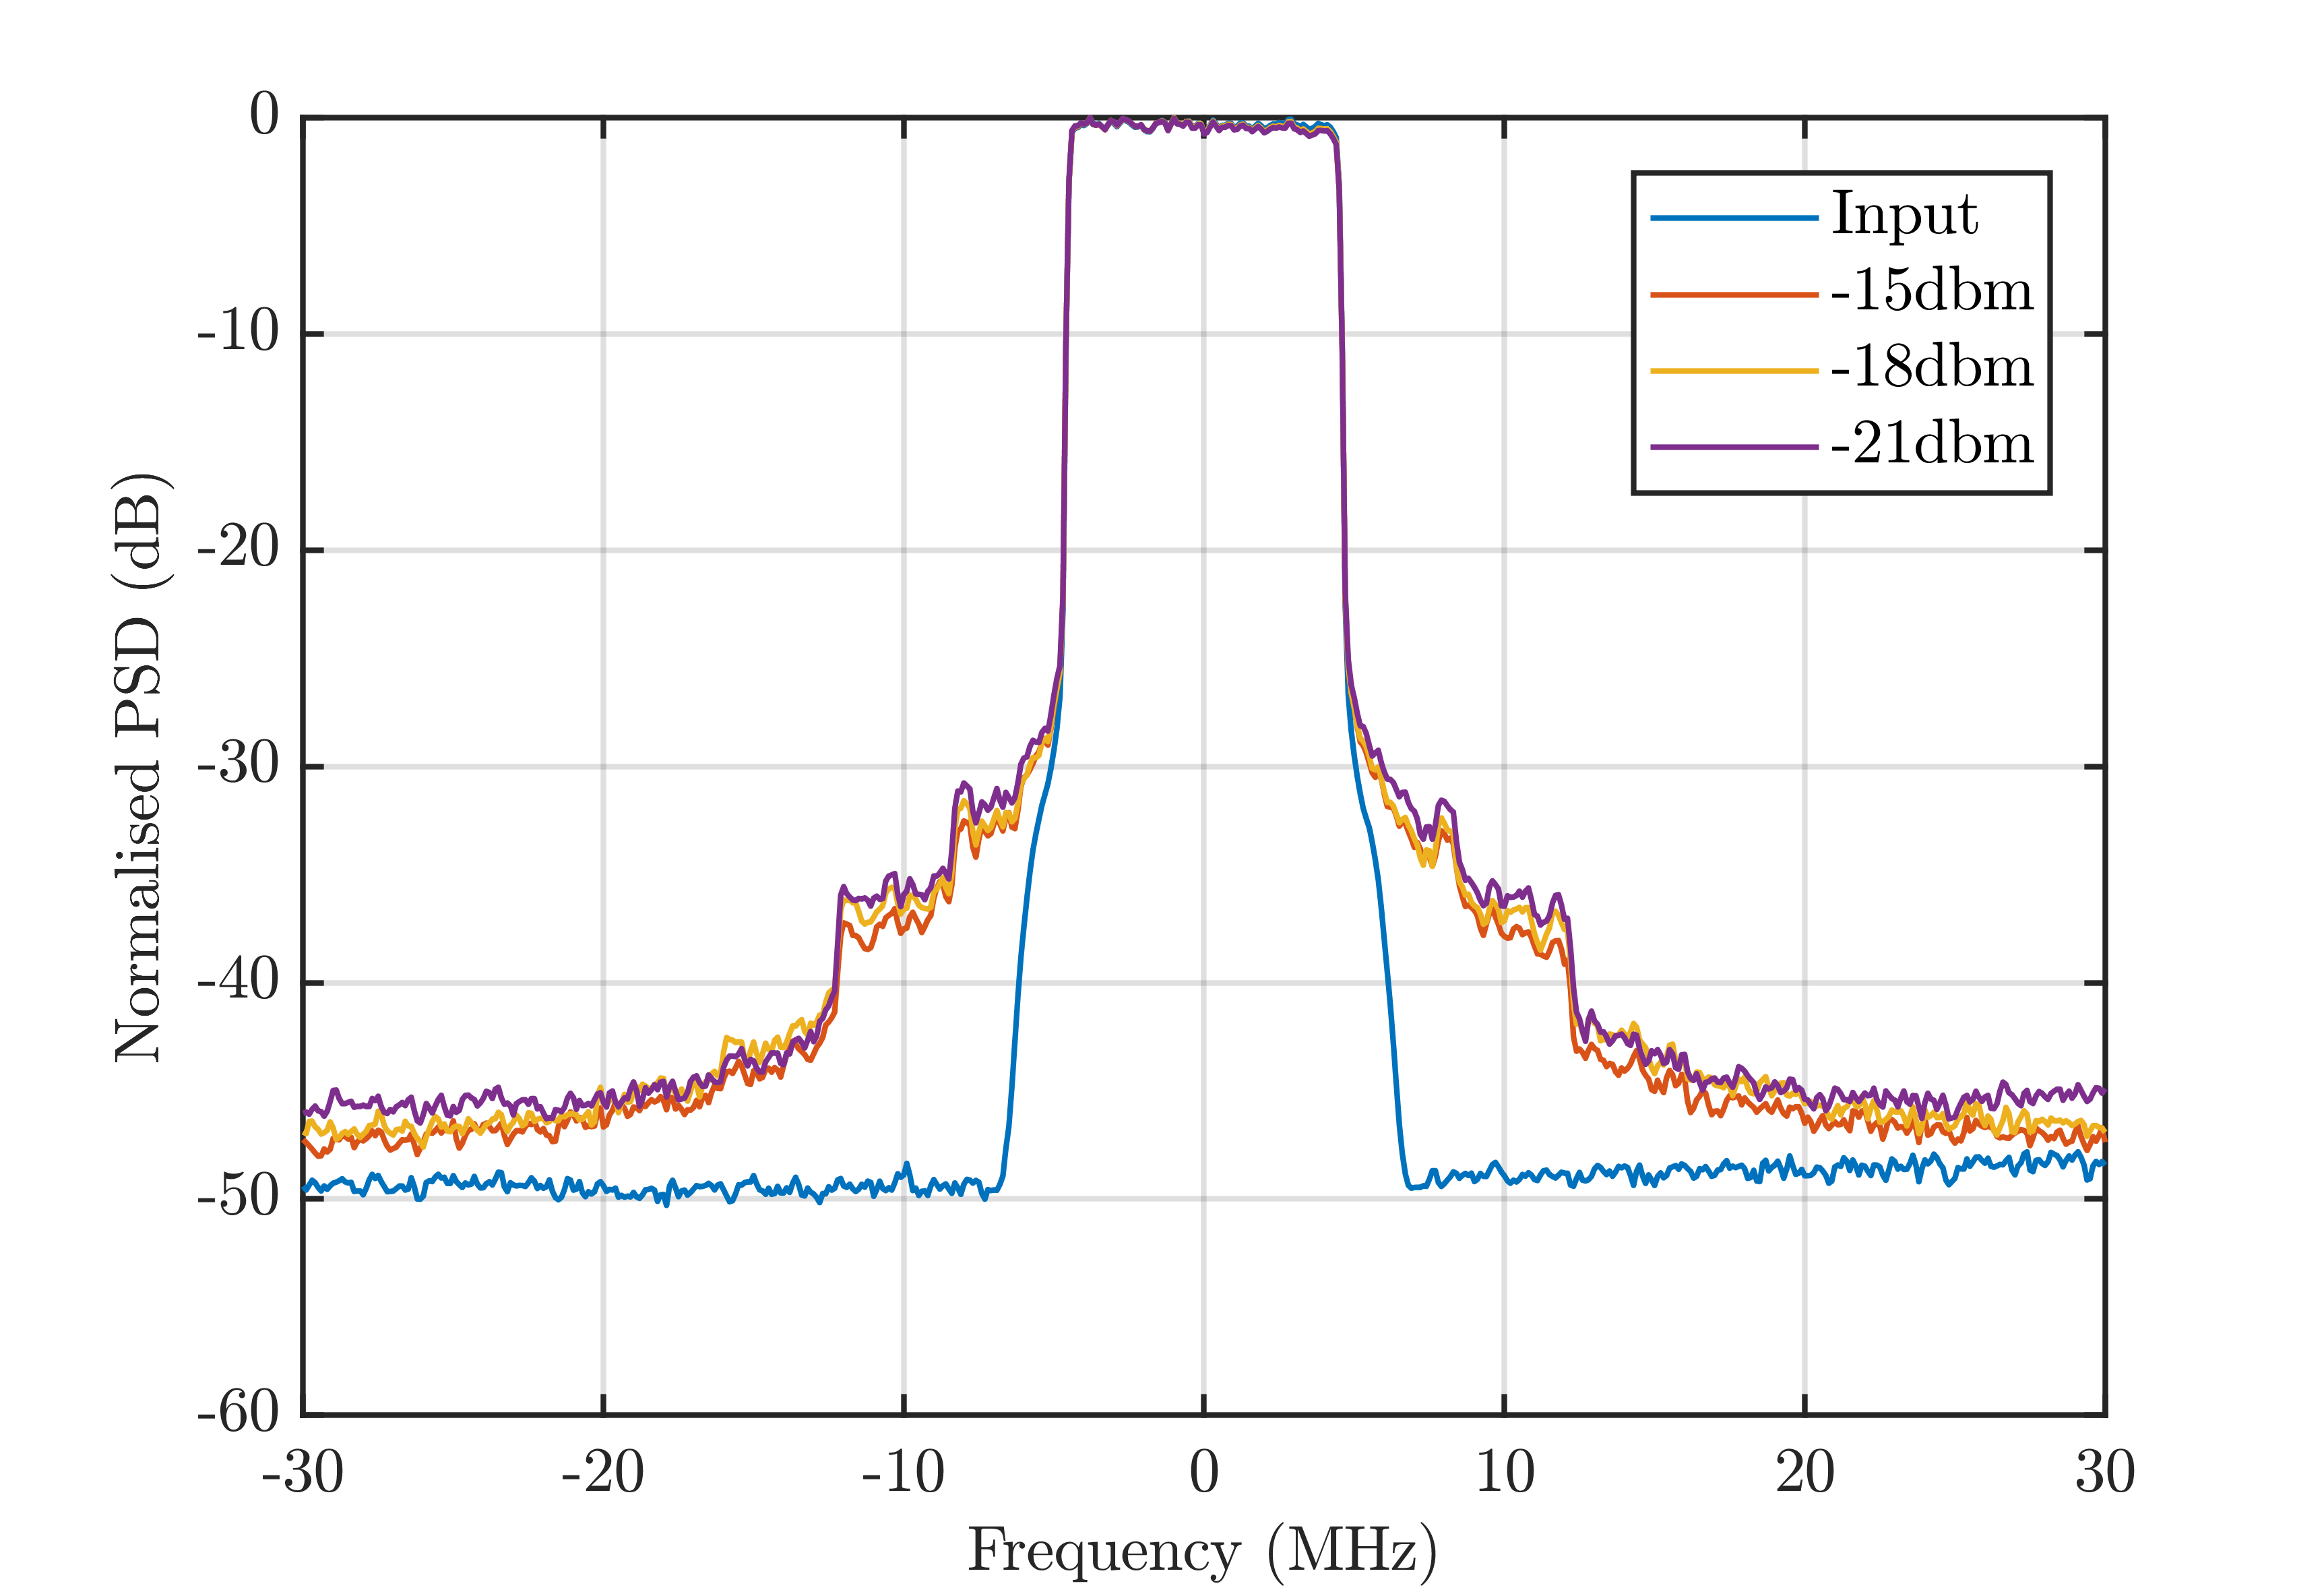
\includegraphics[scale = 0.5]{figures/measurement/cree/psd_cree_amp_no_dpd.png}
	\caption{PSD of amplifier}
    \label{fig:cree_amam1}
  \end{minipage}
  \hfill
  \begin{minipage}[b]{0.4\textwidth}
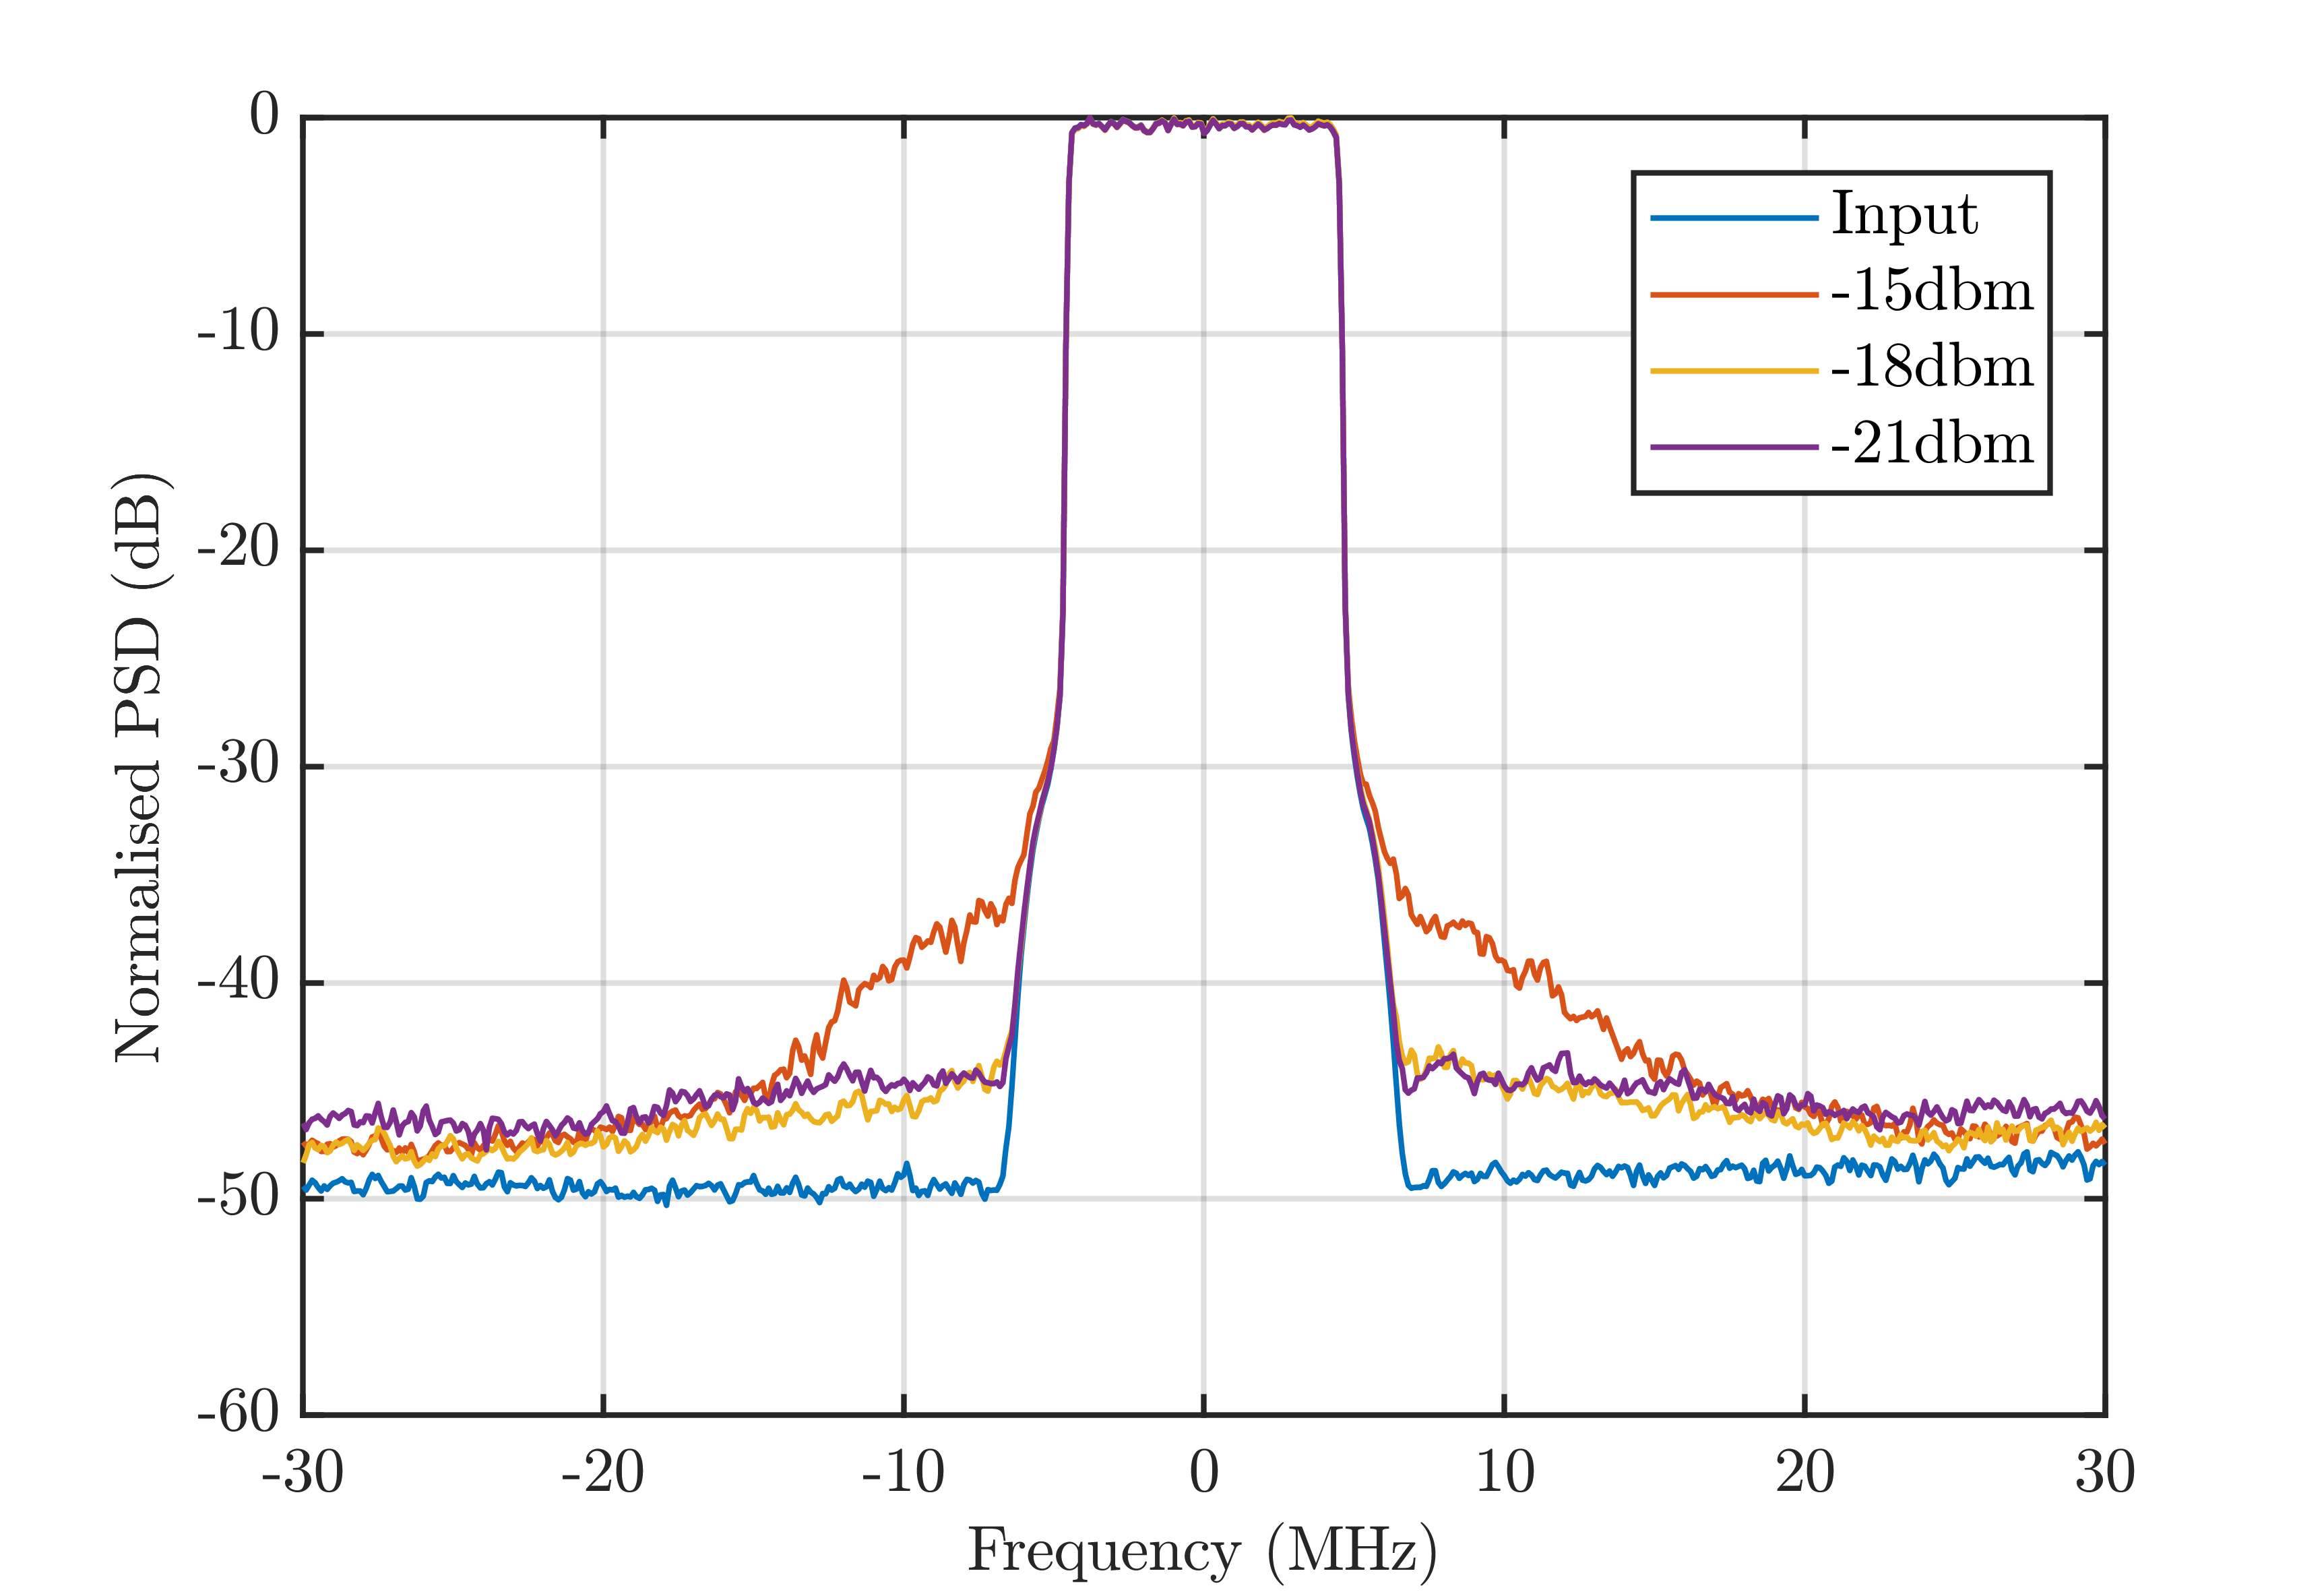
\includegraphics[scale = 0.5]{figures/measurement/cree/psd_cree_amp_with_dpd.png}
\caption{PSD of amplifier with DPD}
    \label{fig:cree_amam2}
  \end{minipage}
\end{figure}

%%%%%%%%%%%%%%%%%%%%%%%%%%%%%%%%%%%%%%%%%%%%%%%%%%%%%%%%%%%%%%%%%%%%%%%%%%%%%%%%%%%%%%%%%%%%%%%%%%%%%%%%%%%%%%%%%%%
\subsubsection{With one antenna}


\begin{figure}[H]
\centering 
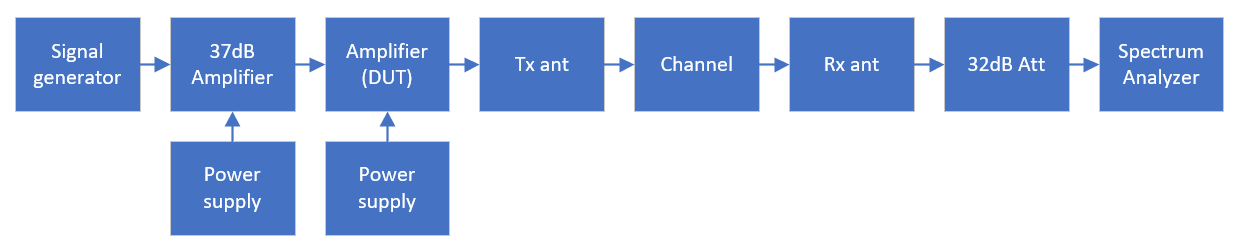
\includegraphics[scale = 0.5]{figures/measurement/cree/one2one_draw.png}
\caption{Measurement setup using one tx antenna}
\label{fig:Meas_setup_draw_cree1}
\end{figure} 


\begin{figure}[H]
\centering 
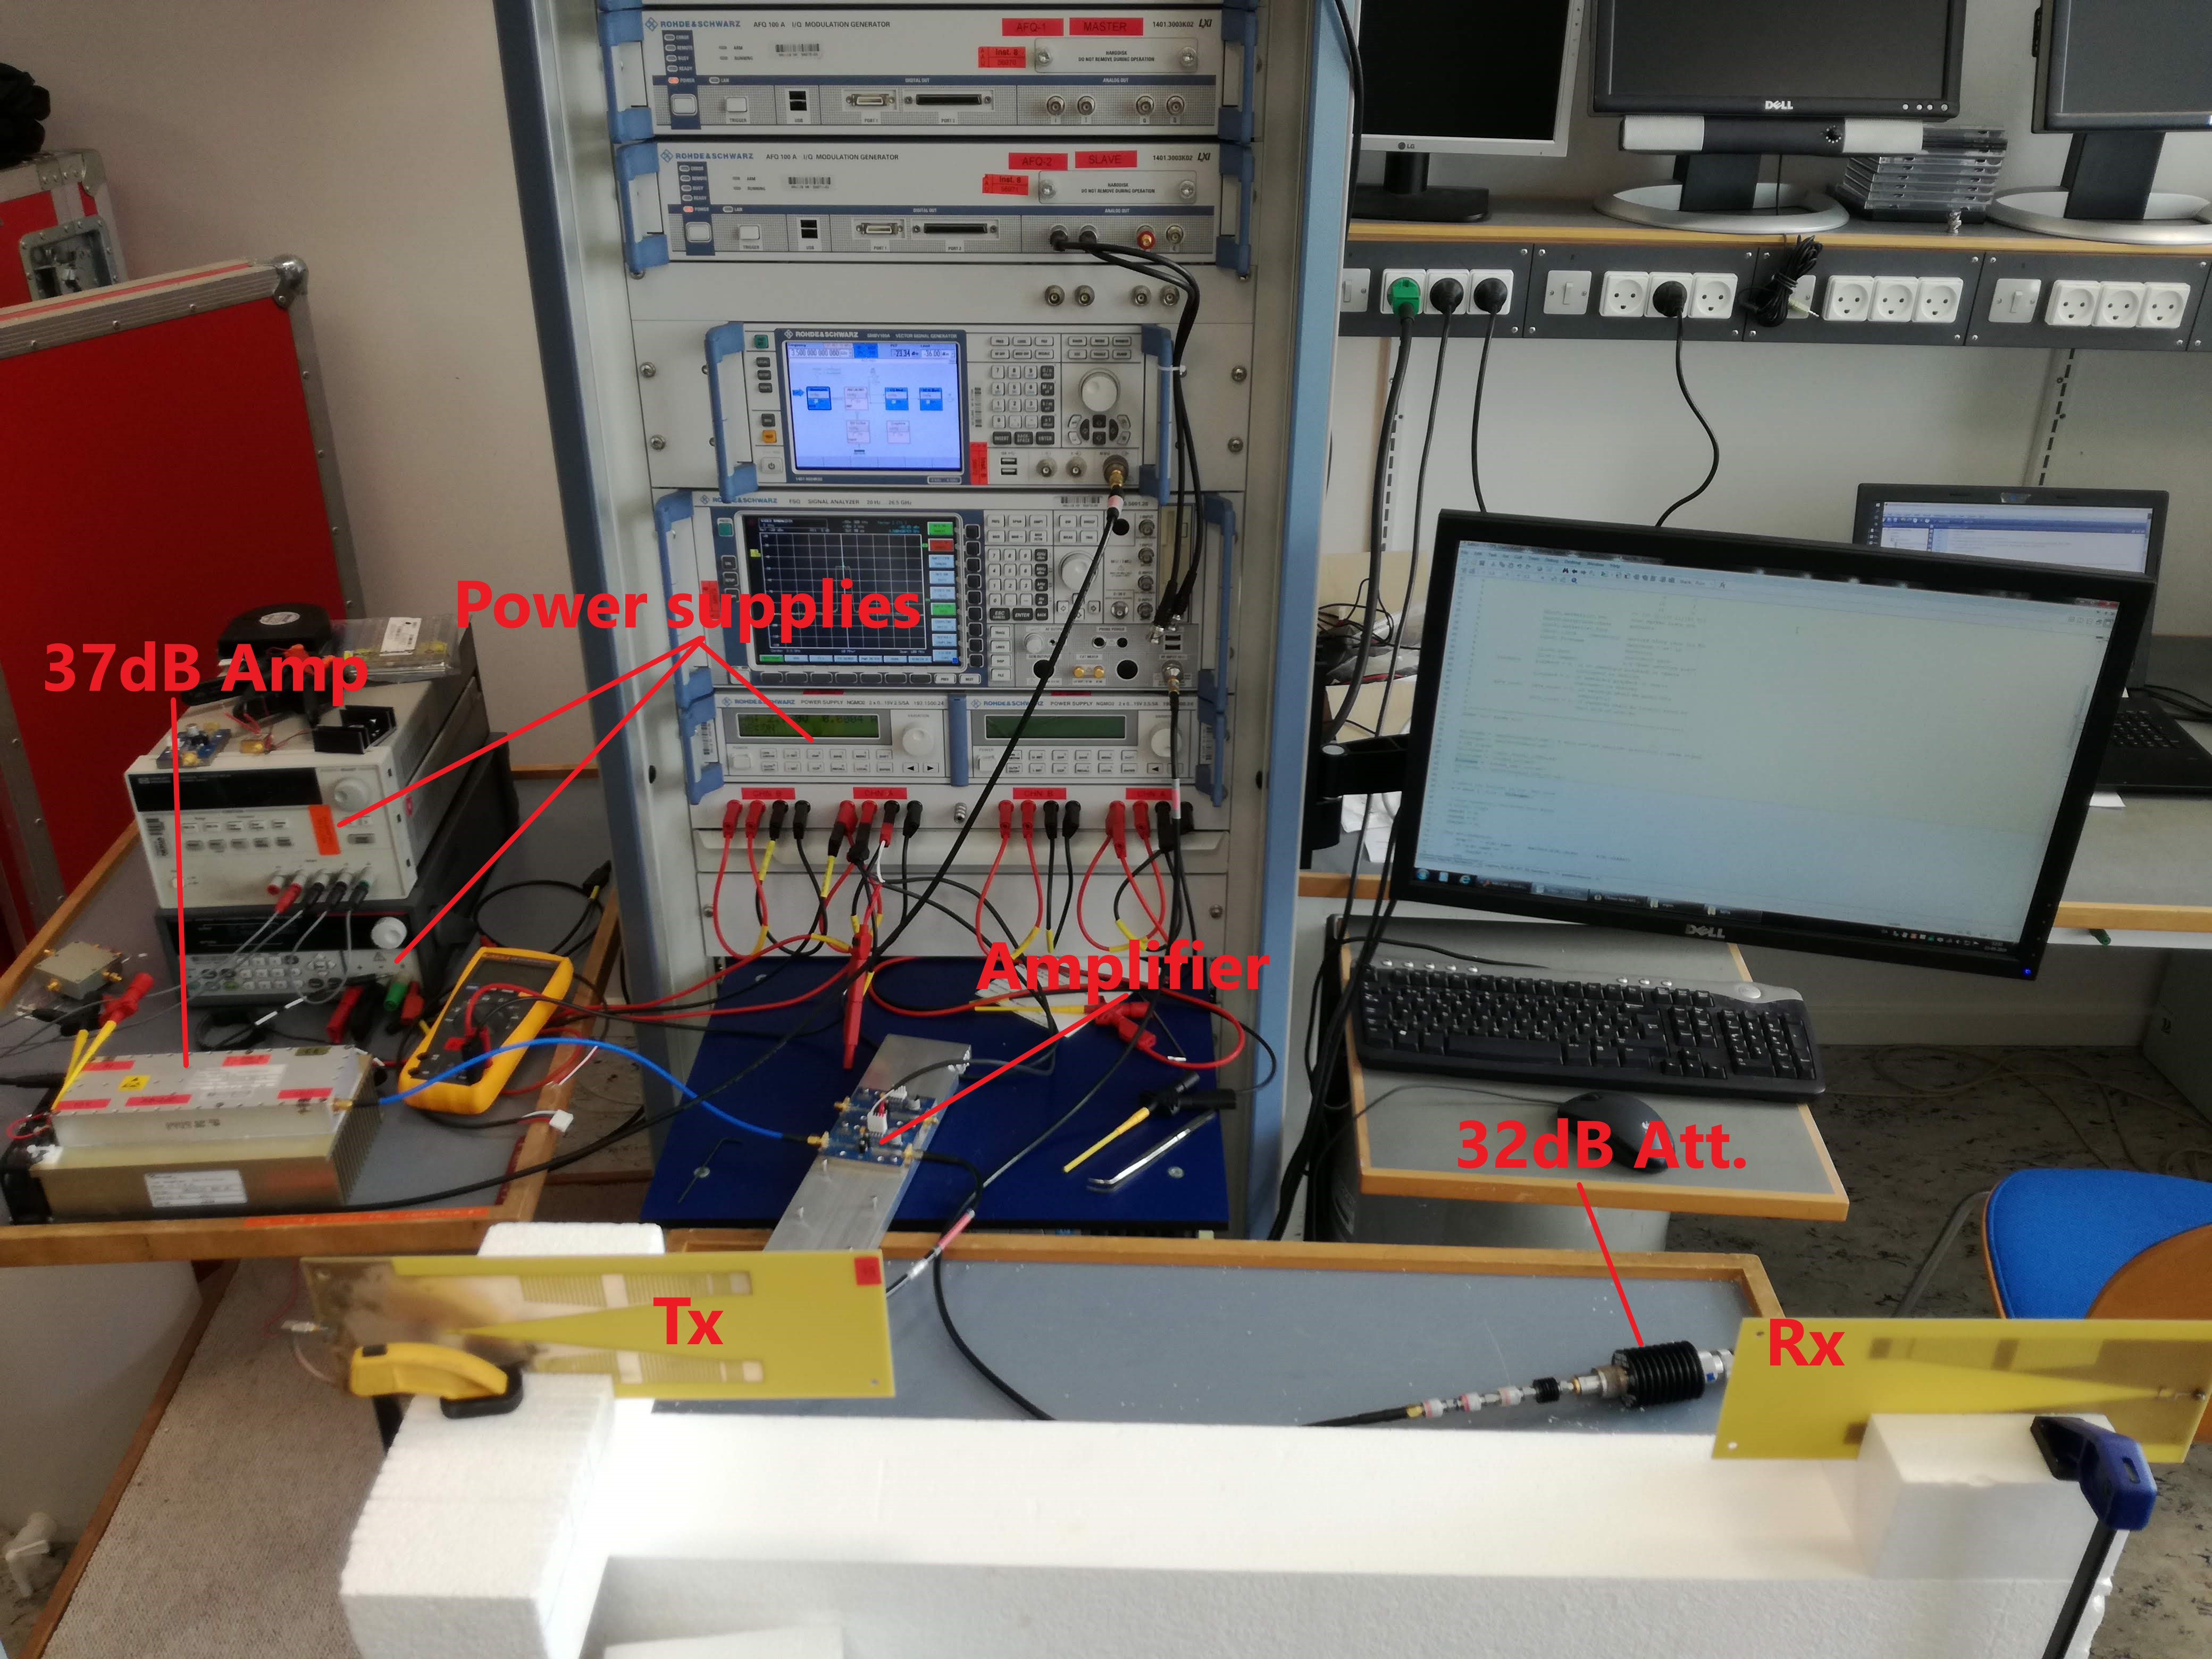
\includegraphics[scale = 0.1]{figures/measurement/cree/one2one.jpg}
\caption{Picture of measurement setup using one tx antenna}
\label{fig:Meas_setup_cree1}
\end{figure} 


\begin{figure}[H]
  \centering
  \begin{minipage}[b]{0.5\textwidth}
	\includegraphics[scale = 0.5]{figures/measurement/cree/amam_one_ant.png}
	\caption{AM/AM of amplifier with one Tx and one Rx antenna}
    \label{fig:cree_amam_one_ant}
  \end{minipage}
  \hfill
  \begin{minipage}[b]{0.4\textwidth}
\includegraphics[scale = 0.5]{figures/measurement/cree/psd_one_ant.png}
\caption{PSD of amplifier with one Tx and one Rx antenna}
    \label{fig:cree_psd_one_ant}
  \end{minipage}
\end{figure}
%%%%%%%%%%%%%%%%%%%%%%%%%%%%%%%%%%%%%%%%%%%%%%%%%%%%%%%%%%%%%%%%%%%%%%%%%%%%%%%%%%%%%%%%%%%%%%%%%%%%%%%%%%%%%%%%%
\subsubsection{With two antennas}

\begin{figure}[H]
\centering 
\includegraphics[scale = 0.4]{figures/measurement/cree/two2one_draw.png}
\caption{Measurement setup using two tx antenna}
\label{fig:Meas_setup_draw_cree1}
\end{figure} 


\begin{figure}[H]
\centering 
\includegraphics[scale = 0.1]{figures/measurement/cree/two2one.jpg}
\caption{Picture of measurement setup using two tx antenna}
\label{fig:Meas_setup_cree1}
\end{figure} 

\begin{figure}[H]
  \centering
  \begin{minipage}[b]{0.5\textwidth}
	\includegraphics[scale = 0.5]{figures/measurement/cree/two/amam_two_ant_0p1.png}
	\caption{AM/AM of amplifier with two Tx antenna spaced $0.1\lambda$ and one Rx antenna}
    \label{fig:cree_amam_one_ant}
  \end{minipage}
  \hfill
  \begin{minipage}[b]{0.4\textwidth}
\includegraphics[scale = 0.5]{figures/measurement/cree/two/psd_two_ant_0p1.png}
\caption{PSD of amplifier with two Tx antenna spaced $0.1\lambda$ and one Rx antenna}
    \label{fig:cree_psd_one_ant}
  \end{minipage}
\end{figure}

\begin{figure}[H]
  \centering
  \begin{minipage}[b]{0.5\textwidth}
	\includegraphics[scale = 0.5]{figures/measurement/cree/two/amam_two_ant_0p2.png}
	\caption{AM/AM of amplifier with two Tx antenna spaced $0.2\lambda$ and one Rx antenna}
    \label{fig:cree_amam_two_ant1}
  \end{minipage}
  \hfill
  \begin{minipage}[b]{0.4\textwidth}
\includegraphics[scale = 0.5]{figures/measurement/cree/two/psd_two_ant_0p2.png}
\caption{PSD of amplifier with two Tx antenna spaced $0.2\lambda$ and one Rx antenna}
    \label{fig:cree_psd_two_ant1}
  \end{minipage}
\end{figure}

\begin{figure}[H]
  \centering
  \begin{minipage}[b]{0.5\textwidth}
	\includegraphics[scale = 0.5]{figures/measurement/cree/two/amam_two_ant_0p3.png}
	\caption{AM/AM of amplifier with two Tx antenna spaced $0.3\lambda$ and one Rx antenna}
    \label{fig:cree_amam_two_ant2}
  \end{minipage}
  \hfill
  \begin{minipage}[b]{0.4\textwidth}
\includegraphics[scale = 0.5]{figures/measurement/cree/two/psd_two_ant_0p3.png}
\caption{PSD of amplifier with two Tx antenna spaced $0.3\lambda$ and one Rx antenna}
    \label{fig:cree_psd_two_ant2}
  \end{minipage}
\end{figure}

\begin{figure}[H]
  \centering
  \begin{minipage}[b]{0.5\textwidth}
	\includegraphics[scale = 0.5]{figures/measurement/cree/two/amam_two_ant_0p4.png}
	\caption{AM/AM of amplifier with two Tx antenna spaced $0.4\lambda$ and one Rx antenna}
    \label{fig:cree_amam_two_ant3}
  \end{minipage}
  \hfill
  \begin{minipage}[b]{0.4\textwidth}
\includegraphics[scale = 0.5]{figures/measurement/cree/two/psd_two_ant_0p4.png}
\caption{PSD of amplifier with two Tx antenna spaced $0.4\lambda$ and one Rx antenna}
    \label{fig:cree_psd_two_ant3}
  \end{minipage}
\end{figure}

\begin{figure}[H]
  \centering
  \begin{minipage}[b]{0.5\textwidth}
	\includegraphics[scale = 0.5]{figures/measurement/cree/two/amam_two_ant_0p5.png}
	\caption{AM/AM of amplifier with two Tx antenna spaced $0.5\lambda$ and one Rx antenna}
    \label{fig:cree_amam_two_ant4}
  \end{minipage}
  \hfill
  \begin{minipage}[b]{0.4\textwidth}
\includegraphics[scale = 0.5]{figures/measurement/cree/two/psd_two_ant_0p5.png}
\caption{PSD of amplifier with two Tx antenna spaced $0.5\lambda$ and one Rx antenna}
    \label{fig:cree_psd_two_ant4}
  \end{minipage}
\end{figure}

\begin{figure}[H]
  \centering
  \begin{minipage}[b]{0.5\textwidth}
	\includegraphics[scale = 0.5]{figures/measurement/cree/two/amam_two_ant_0p6.png}
	\caption{AM/AM of amplifier with two Tx antenna spaced $0.6\lambda$ and one Rx antenna}
    \label{fig:cree_amam_two_ant5}
  \end{minipage}
  \hfill
  \begin{minipage}[b]{0.4\textwidth}
\includegraphics[scale = 0.5]{figures/measurement/cree/two/psd_two_ant_0p1.png}
\caption{PSD of amplifier with two Tx antenna spaced $0.6\lambda$ and one Rx antenna}
    \label{fig:cree_psd_two_ant5}
  \end{minipage}
\end{figure}

\begin{figure}[H]
  \centering
  \begin{minipage}[b]{0.5\textwidth}
	\includegraphics[scale = 0.5]{figures/measurement/cree/two/amam_two_ant_1p0.png}
	\caption{AM/AM of amplifier with two Tx antenna spaced $1\lambda$ and one Rx antenna}
    \label{fig:cree_amam_two_ant6}
  \end{minipage}
  \hfill
  \begin{minipage}[b]{0.4\textwidth}
\includegraphics[scale = 0.5]{figures/measurement/cree/two/psd_two_ant_1p0.png}
\caption{PSD of amplifier with two Tx antenna spaced $1\lambda$ and one Rx antenna}
    \label{fig:cree_psd_two_ant6}
  \end{minipage}
\end{figure}



%%%%%%%%%%%%%%%%%%%%%%%%%%%%%%%%%%%%%%%%%%%%%%%%%%%%%%%%%%%%%%%%%%%%%%%%%%%%%%%%%%%%%%%%%%%%%%%%%%%%%%%%%%%%%%%%%
\subsubsection{With four antennas}


\begin{figure}[H]
\centering 
\includegraphics[scale = 0.08]{figures/measurement/cree/four2one.jpg}
\caption{Picture of measurement setup using four tx antenna}
\label{fig:Meas_setup_cree1}
\end{figure} 


\begin{figure}[H]
  \centering
  \begin{minipage}[b]{0.5\textwidth}
	\includegraphics[scale = 0.5]{figures/measurement/cree/four/amam_four_ant_0p1.png}
	\caption{AM/AM of amplifier with four Tx antenna spaced $0.1\lambda$ and one Rx antenna}
    \label{fig:cree_amam_one_ant}
  \end{minipage}
  \hfill
  \begin{minipage}[b]{0.4\textwidth}
\includegraphics[scale = 0.5]{figures/measurement/cree/four/psd_four_ant_0p1.png}
\caption{PSD of amplifier with four Tx antenna spaced $0.1\lambda$ and one Rx antenna}
    \label{fig:cree_psd_one_ant}
  \end{minipage}
\end{figure}

\begin{figure}[H]
  \centering
  \begin{minipage}[b]{0.5\textwidth}
	\includegraphics[scale = 0.5]{figures/measurement/cree/four/amam_four_ant_0p2.png}
	\caption{AM/AM of amplifier with four Tx antenna spaced $0.2\lambda$ and one Rx antenna}
    \label{fig:cree_amam_four_ant1}
  \end{minipage}
  \hfill
  \begin{minipage}[b]{0.4\textwidth}
\includegraphics[scale = 0.5]{figures/measurement/cree/four/psd_four_ant_0p2.png}
\caption{PSD of amplifier with four Tx antenna spaced $0.2\lambda$ and one Rx antenna}
    \label{fig:cree_psd_four_ant1}
  \end{minipage}
\end{figure}

\begin{figure}[H]
  \centering
  \begin{minipage}[b]{0.5\textwidth}
	\includegraphics[scale = 0.5]{figures/measurement/cree/four/amam_four_ant_0p3.png}
	\caption{AM/AM of amplifier with four Tx antenna spaced $0.3\lambda$ and one Rx antenna}
    \label{fig:cree_amam_four_ant2}
  \end{minipage}
  \hfill
  \begin{minipage}[b]{0.4\textwidth}
\includegraphics[scale = 0.5]{figures/measurement/cree/four/psd_four_ant_0p3.png}
\caption{PSD of amplifier with four Tx antenna spaced $0.3\lambda$ and one Rx antenna}
    \label{fig:cree_psd_four_ant2}
  \end{minipage}
\end{figure}

\begin{figure}[H]
  \centering
  \begin{minipage}[b]{0.5\textwidth}
	\includegraphics[scale = 0.5]{figures/measurement/cree/four/amam_four_ant_0p4.png}
	\caption{AM/AM of amplifier with four Tx antenna spaced $0.4\lambda$ and one Rx antenna}
    \label{fig:cree_amam_four_ant3}
  \end{minipage}
  \hfill
  \begin{minipage}[b]{0.4\textwidth}
\includegraphics[scale = 0.5]{figures/measurement/cree/four/psd_four_ant_0p4.png}
\caption{PSD of amplifier with four Tx antenna spaced $0.4\lambda$ and one Rx antenna}
    \label{fig:cree_psd_four_ant3}
  \end{minipage}
\end{figure}

\begin{figure}[H]
  \centering
  \begin{minipage}[b]{0.5\textwidth}
	\includegraphics[scale = 0.5]{figures/measurement/cree/four/amam_four_ant_0p5.png}
	\caption{AM/AM of amplifier with four Tx antenna spaced $0.5\lambda$ and one Rx antenna}
    \label{fig:cree_amam_four_ant4}
  \end{minipage}
  \hfill
  \begin{minipage}[b]{0.4\textwidth}
\includegraphics[scale = 0.5]{figures/measurement/cree/four/psd_four_ant_0p5.png}
\caption{PSD of amplifier with four Tx antenna spaced $0.5\lambda$ and one Rx antenna}
    \label{fig:cree_psd_four_ant4}
  \end{minipage}
\end{figure}

\begin{figure}[H]
  \centering
  \begin{minipage}[b]{0.5\textwidth}
	\includegraphics[scale = 0.5]{figures/measurement/cree/four/amam_four_ant_0p6.png}
	\caption{AM/AM of amplifier with four Tx antenna spaced $0.6\lambda$ and one Rx antenna}
    \label{fig:cree_amam_four_ant5}
  \end{minipage}
  \hfill
  \begin{minipage}[b]{0.4\textwidth}
\includegraphics[scale = 0.5]{figures/measurement/cree/four/psd_four_ant_0p1.png}
\caption{PSD of amplifier with four Tx antenna spaced $0.6\lambda$ and one Rx antenna}
    \label{fig:cree_psd_four_ant5}
  \end{minipage}
\end{figure}





